%%%%%%%%%%%%%%%%%%%%%%%%%%%%%%%%%%%%%%%%%
% Masters/Doctoral Thesis 
% LaTeX Template
% Version 2.5 (27/8/17)
%
% This template was downloaded from:
% http://www.LaTeXTemplates.com
%
% Version 2.x major modifications by:
% Vel (vel@latextemplates.com)
%
% This template is based on a template by:
% Steve Gunn (http://users.ecs.soton.ac.uk/srg/softwaretools/document/templates/)
% Sunil Patel (http://www.sunilpatel.co.uk/thesis-template/)
%
% Template license:
% CC BY-NC-SA 3.0 (http://creativecommons.org/licenses/by-nc-sa/3.0/)
%
%%%%%%%%%%%%%%%%%%%%%%%%%%%%%%%%%%%%%%%%%

%----------------------------------------------------------------------------------------
%	PACKAGES AND OTHER DOCUMENT CONFIGURATIONS
%----------------------------------------------------------------------------------------

\documentclass[
10pt, % The default document font size, options: 10pt, 11pt, 12pt
%oneside, % Two side (alternating margins) for binding by default, uncomment to switch to one side
english, % ngerman for German
singlespacing, % Single line spacing, alternatives: onehalfspacing or doublespacing
%draft, % Uncomment to enable draft mode (no pictures, no links, overfull hboxes indicated)
%nolistspacing, % If the document is onehalfspacing or doublespacing, uncomment this to set spacing in lists to single
%liststotoc, % Uncomment to add the list of figures/tables/etc to the table of contents
%toctotoc, % Uncomment to add the main table of contents to the table of contents
%parskip, % Uncomment to add space between paragraphs
% nohyperref, % Uncomment to not load the hyperref package
headsepline, % Uncomment to get a line under the header
%chapterinoneline, % Uncomment to place the chapter title next to the number on one line
%consistentlayout, % Uncomment to change the layout of the declaration, abstract and acknowledgements pages to match the default layout
]{MastersDoctoralThesis} % The class file specifying the document structure

\usepackage[utf8]{inputenc} % Required for inputting international characters
\usepackage[T1]{fontenc} % Output font encoding for international characters

\usepackage{mathpazo} % Use the Palatino font by default

\usepackage[backend=bibtex,style=ieee]{biblatex} % Use the bibtex backend with the authoryear citation style (which resembles APA)

% \usepackage[block=ragged,natbib=true]{biblatex}

\usepackage{subcaption} % for subfigures

\usepackage{tikz}
\usetikzlibrary{positioning,arrows,fit,backgrounds, patterns}

\usepackage[super]{nth}

\addbibresource{references.bib} % The filename of the bibliography

\usepackage[autostyle=true]{csquotes} % Required to generate language-dependent quotes in the bibliography

\usepackage{layout}

\usepackage{graphicx}
\usepackage{bm}
\usepackage{wrapfig}
\usepackage{amsmath}
\usepackage{diagbox}
\usepackage{makecell}
\usepackage{mathtools}

\usepackage[bookmarks=false]{hyperref}
\usepackage{scrextend}
\usepackage{fullpage}
\usepackage{amssymb}
\usepackage{tabularx}
\usepackage[linesnumbered,ruled]{algorithm2e}
\usepackage{csvsimple, booktabs, siunitx, xstring}
\usepackage{import}
\usepackage[skip=10pt]{caption}
\usepackage{array, multirow}
\usepackage{arydshln}
\usepackage{float}


%----------------------------------------------------------------------------------------
%	TOC SETTINGS
%----------------------------------------------------------------------------------------

\setcounter{secnumdepth}{2} % only chapter and sections and subsections will be numbered
\setcounter{tocdepth}{2}    % entries down to \subsections in the TOC

%----------------------------------------------------------------------------------------
%	MARGIN SETTINGS
%----------------------------------------------------------------------------------------

\geometry{
	paper=a4paper, % Change to letterpaper for US letter
	inner=2.5cm, % Inner margin
	outer=3.8cm, % Outer margin
	bindingoffset=.5cm, % Binding offset
	top=1.5cm, % Top margin
	bottom=1.5cm, % Bottom margin
	%showframe, % Uncomment to show how the type block is set on the page
}

% \hyphenation{Mou-gia-ka-kou}

%----------------------------------------------------------------------------------------
%	THESIS INFORMATION
%----------------------------------------------------------------------------------------

\thesistitle{Annotation of Medical Videos and Volumes using Sparse Point-wise Supervision}
\supervisor{Prof. Dr. \textsc{Sznitman} Raphael} % Your supervisor's name, this is used in the title page, print it elsewhere with \supname
\coadvisor{Prof. Dr. \textsc{Favaro} Paolo} % Your examiner's name, this is not currently used anywhere in the template, print it elsewhere with \examname
\degree{Doctor of Philosophy in XXX} % Your degree name, this is used in the title page and abstract, print it elsewhere with \degreename
\author{\textsc{Surname} FirstName} % Your name, this is used in the title page and abstract, print it elsewhere with \authorname

\matriculation{00-000-000} % Your matriculation number, this is not currently used anywhere in the template, print it elsewhere with \matriculationnum

\subject{SUBJECT} % Your subject area, this is not currently used anywhere in the template, print it elsewhere with \\subjectname
\keywords{keyword1, keyword2} % Keywords for your thesis, this is not currently used anywhere in the template, print it elsewhere with \keywordnames
\university{University of Bern} % Your university's name and URL, this is used in the title page and abstract, print it elsewhere with \univname
\department{Faculty of XXX} % Your department's name and URL, this is used in the title page and abstract, print it elsewhere with \deptname
\group{Group Name} % Your research group's name and URL, this is used in the title page, print it elsewhere with \groupname
\faculty{Graduate School for Cellular and Biomedical Sciences} % Your faculty's name and URL, this is used in the title page and abstract, print it elsewhere with \facname

\newcommand*{\resetfigpath}[1]{
    \graphicspath{{chapters/#1/pics/}}
}

\graphicspath{{pics/}}

\begin{document}

\frontmatter % Use roman page numbering style (i, ii, iii, iv...) for the pre-content pages

\pagestyle{plain} % Default to the plain heading style until the thesis style is called for the body content

%----------------------------------------------------------------------------------------
%	TITLE PAGE 1
%----------------------------------------------------------------------------------------

\begin{titlepage}

\hfill{
\includegraphics[width=4.5cm]{Logo-unibe}}

\begin{center}

\vspace*{0.5cm}
{\Large \facname \\ \textsc{\univname} \par}\vspace{1cm} % University name

{\huge \bfseries \ttitle\par}\vspace{1cm} % Thesis title
\large{PhD Thesis submitted by}\vspace{0.5cm}

{\Large \bfseries \authorname \par}\vspace{0.5cm}

\large{from }{\Large \bfseries Place of Origin \& Canton \par}\vspace{0.5cm}

\large{from }{\Large \bfseries Country of Origin \par}\vspace{0.5cm}

\large{for the degree of XXX}\vspace{0.5cm}
 
\vfill

\large{Supervisor \\ \supname \\ Supervisor Institute/Department of YYY}\vspace{0.5cm}

\large{Co-advisor \\ \examname \\  Co-advisor Institute/Department of YYY}\vspace{0.5cm}
\large{Mentor \\ \examname \\  Co-advisor Institute/Department of YYY}\vspace{0.5cm}

% % this is needed for the publication at the university of bern library
% \footnotesize{Original document saved on the web server of the University Library of Bern\\}
% 
\includegraphics[width=1.5cm]{cc88x31}\\
% \footnotesize{This work is licensed under a \href{https://creativecommons.org/licenses/by-nc-nd/2.5/ch/}{Creative Commons Attribution-NonCommercial-NoDerivs 2.5 Switzerland License}.}
\end{center}
\end{titlepage}
\cleardoublepage

% %----------------------------------------------------------------------------------------
% %	TITLE PAGES 2
% %----------------------------------------------------------------------------------------
% {
% \pagenumbering{gobble}
% \vspace*{5cm}
% \begin{center}
% \textbf{\Large{Copyright Notice}}
% \end{center}

% \noindent This document is licensed under the Creative Commons Attribution-Non-Commercial-No derivative works 2.5 Switzerland. 
% \url{http://creativecommons.org/licenses/by-nc-nd/2.5/ch/} \\

% \noindent\textbf{\large{You are free:}}\\
% \noindent\textbf{Share.} copy and redistribute the material in any medium or format. \\

% \noindent\textbf{\large{Under the following conditions:}}\\
% \textbf{Attribution.} You must give appropriate credit, provide a link to the license, and indicate if changes were made. You may do so in any reasonable manner, but not in any way that suggests the licensor endorses you or your use.  \\
% \textbf{Non-Commercial.} You may not use the material for commercial purposes.  \\
% \textbf{No derivative works.} If you remix, transform, or build upon the material, you may not distribute the modified material.  \\

% \noindent For any reuse or distribution, you must make clear to others the license terms of this work.  \\

% \noindent Any of these conditions can be waived if you get permission from the copyright holder. \\

% \noindent Nothing in this license impairs or restricts the author’s moral rights according to Swiss law. \\

% \noindent The detailed license agreement can be found at: \url{http://creativecommons.org/licenses/by-nc-nd/2.5/ch/legalcode.de}
% \cleardoublepage
% \pagenumbering{roman}
% % \clearpage

%----------------------------------------------------------------------------------------
%	TITLE PAGES 3
%----------------------------------------------------------------------------------------

\cleardoublepage

%----------------------------------------------------------------------------------------
%	TITLE PAGES 4
%----------------------------------------------------------------------------------------

\vspace*{\fill}

\noindent Accepted by the Faculty of Medicine, the Faculty of Science and the Vetsuisse Faculty of the University of Bern at the request of the Graduate School for Cellular and Biomedical Sciences

\vspace{3cm}

\noindent Bern, 	Dean of the Faculty of Medicine

\vspace{3cm}

\noindent Bern, 	Dean of the Faculty of Science

\vspace{3cm}

\noindent Bern, 	Dean of the Vetsuisse Faculty Bern

\vspace{3cm}

\vspace*{\fill}

\cleardoublepage

%----------------------------------------------------------------------------------------
%	ABSTRACT PAGE
%----------------------------------------------------------------------------------------

\begin{abstract}
\addchaptertocentry{\abstractname} % Add the abstract to the table of contents
Lorem ipsum dolor sit amet, consectetur adipiscing elit. Nam bibendum, mi non lacinia aliquet, orci nisi commodo ex, ac malesuada nunc libero eget metus. Proin vel enim risus. Nullam lobortis posuere sodales. Quisque ac placerat sapien. Praesent in pulvinar dolor. Pellentesque faucibus quam at dui consectetur scelerisque. Donec laoreet pharetra neque, id cursus metus venenatis eu. Quisque tempor molestie velit, ac euismod ligula ullamcorper a. Aliquam lacus ligula, ultrices id vehicula et, hendrerit non turpis. Phasellus molestie erat quis sem iaculis, sed posuere metus tempus. Nullam suscipit lorem et accumsan convallis. Cras eleifend mauris ultrices nunc hendrerit condimentum. 
\\
\textbf{Keywords --} \keywordnames
\\ ~ \\ ~ \\ ~ \\
\end{abstract}

%----------------------------------------------------------------------------------------
%	ACKNOWLEDGEMENTS
%----------------------------------------------------------------------------------------

\begin{acknowledgements}
\addchaptertocentry{\acknowledgementname} % Add the acknowledgements to the table of contents
Lorem ipsum dolor sit amet, consectetur adipiscing elit. Nam bibendum, mi non lacinia aliquet, orci nisi commodo ex, ac malesuada nunc libero eget metus. Proin vel enim risus. Nullam lobortis posuere sodales. Quisque ac placerat sapien. Praesent in pulvinar dolor. Pellentesque faucibus quam at dui consectetur scelerisque. Donec laoreet pharetra neque, id cursus metus venenatis eu. Quisque tempor molestie velit, ac euismod ligula ullamcorper a. Aliquam lacus ligula, ultrices id vehicula et, hendrerit non turpis. Phasellus molestie erat quis sem iaculis, sed posuere metus tempus. Nullam suscipit lorem et accumsan convallis. Cras eleifend mauris ultrices nunc hendrerit condimentum. 
\end{acknowledgements}

%----------------------------------------------------------------------------------------
%	LIST OF CONTENTS/FIGURES/TABLES PAGES
%----------------------------------------------------------------------------------------

\tableofcontents % Prints the main table of contents

% \listoffigures % Prints the list of figures

% \listoftables % Prints the list of tables

%----------------------------------------------------------------------------------------
%	ABBREVIATIONS
%----------------------------------------------------------------------------------------

\begin{abbreviations}{ll} % Include a list of abbreviations (a table of two columns)
\end{abbreviations}

%----------------------------------------------------------------------------------------
%	DEDICATION
%----------------------------------------------------------------------------------------

\dedicatory{Dedication}

%----------------------------------------------------------------------------------------
%	THESIS CONTENT - CHAPTERS
%----------------------------------------------------------------------------------------

\mainmatter % Begin numeric (1,2,3...) page numbering

\pagestyle{thesis} % Return the page headers back to the "thesis" style

% Include the chapters of the thesis as separate files from the Chapters folder
% Uncomment the lines as you write the chapters

\resetfigpath{1-intro}

\chapter{Introduction}
\label{intro}

The medical imaging field has recently witnessed the revolution of \gls{ai}, a broad discipline that is a part of computer science whose aim is to conceptualize human ``intellectual'' tasks, and produce computer programs that can replicate them, thereby allowing to relieve human beings from tedious and repetitive tasks.
From classification to segmentation tasks, \gls{ai} already provides flexible and efficient tools that greatly facilitate the daily practice of clinicians.
In particular, large quantities of \gls{mri} brain scans are now efficiently and accurately processed by \gls{ai} systems that help clinicians in the diagnosis of pathologies \cite{sun19}.
Similarly, surgical instruments can be segmented automatically and accurately in real-time to allow laparoscopic interventions of the abdominal cavity by means of robotic technology, thereby decreasing the invasiveness of traditional methods \cite{davinci}.

\Gls{ml}, a term that denote a sub-category of \gls{ai}, is grounded on the ``learning by example'' paradigm.
Whereas traditional approaches generally consisted in explicitly formalizing and implementing complex tasks as a combination of simpler programmatic instructions,
\gls{ml} rather considers that a flexible system can learn such instructions automatically through repeated experiences.

Concretely, as a young child can effectively derive the concept of car using a few visual examples, and be able to identify an ``unseen'' car in a complex environment with near-perfect accuracy,
state-of-the-art \gls{ml} methods leverage the same principle.
However, no matter how well-engineered they are, they need, in order to replicate this simple task with comparable accuracy, thousands of examples and counter-examples of images \cite{ILSVRC15}.

In this scenario, collecting such quantity of example images and annotating them is tedious and cumbersome.
In practice, the annotation task is performed by numerous individuals in parallel.
The annotation of medical data, however, adds the following practical difficulties.
First, the task can require a specific medical expertise.
Second, assuming such experts are available and willing to participate to this task, their daily obligations imposes a limited time budget.
These two factors largely explain why the medical field does not benefit from the latest and greatest \gls{ml} technologies used in more generic applications \cite{orting19}.


\section{Proposed annotation protocol and applicability}

In the present thesis, we devise solutions that allow to annotate medical sequences in a fast and intuitive manner, in an attempt to alleviate the bottleneck of scarcity of example data.

In particular, the annotator is presented a video or volumetric sequence that plays on a screen, i.e. the frames unfold in an automatic manner.
As the sequence unfolds, the annotator is asked to point at the object of interest using a pointing device, such as a mouse, a tablet pen, or an eye-gaze tracker.
In contrast with the traditional approach, where the object must be manually segmented on each frame individually, the proposed protocol drastically reduces the annotation time.
In essence, our contribution ambitions an annotation time equal to the duration of the video/volume playback.
For example, assuming the sequence contains $100$ frames playing at $5fps$, the total annotation time is $20$ seconds.
In comparison, the traditional pixel-wise annotation task of a sequence of similar size could take anywhere from $10$ min. to $1$ hour.

Concretely, we set the following requirements on the annotation protocol:
\begin{itemize}
  \item The annotator does not need to manually change the frame being annotated, e.g. by hitting a forward or backward key. The sequence automatically unfolds according to a specified frame-rate.
  \item The annotator handles a single pointing device, which he/she uses to indicate the location of the object of interest.
  \item The annotator must be able to watch and annotate the sequence in a single go, i.e. he/she does not need to review annotations and modify them manually afterwards.
\end{itemize}

The segmentation method must be functional in a variety of situations, namely produce acceptable accuracy for:
\begin{itemize}
  \item Both videos and volumetric sequences.
  \item Both color and grayscale images.
  \item Various kind of image modality, e.g. \gls{mri} and \gls{ct}.
  \item Various levels of noise, perturbations, and lightning artifacts.
  \item Various nature of object, i.e. size, shape, appearance.
  \item The object can be made of several parts that are not immediately contiguous, i.e. an \gls{mri} brain scan with several tumors.
\end{itemize}

\section{Datasets}

We now introduce the datasets that have been used during the elaboration and testing of the proposed solutions.
Note that as the range of possibilities is huged, we chose to restrict ourselves to $4$ types of sequences. These, however, cover the entirety of the proposed spectrum.

In particular, we now describe them in detail and give each type a short name that will be used in the remaining of this thesis:

\begin{itemize}
  \item \textbf{Tweezer}: Surgical instruments during an endoscopic procedure, where the instrument is object of interest.
    The background is relatively homogeneous, while the instrument moves accross the frame both in translation and rotation.
    The sequences are taken from the MICCAI EndoVision Challenge \cite{EndoChall}.
    Each sequence is around $120$ frames long, i.e. represent $\sim 5s$ of video acquired at $25$ fps.
  \item \textbf{Cochlea}: Volumetric \Gls{ct} scans of the inner-ear where the cochlear labyrinth is to be segmented. These are acquired according to different protocols, and therefore show important variations in gray-scale level, orientation, as well as sizes. Furthermore, the object of interest is composed of different parts that split and merge.
  \item \textbf{Slitlamp}: Microscopic video of the retina where the optic nerve is to be segmented. The videos have been acquired using a slitlamp instrument.
    The optic nerve is of rather small size. The background often shows important artifacts, in the form of yellow and blue beams, which sometime overlap with the object of interest. The movement of the optic nerve is often very jerky.
  \item \textbf{Brain}: Transverse \gls{mri} scans of brains where the tumor is object of interest. The sequences are taken randomly from the Brain Tumor Segmentation Challenge (BRATS) public database \cite{BRATSChall}.
    Scans are acquired using the same \gls{mri} protocol, but with different scanners, thereby showing wide variety of contrast and color.
    The tumors have varying size, colors, and shapes. Sometimes, the same scan shows several tumors on the same slice.

\end{itemize}

In Fig. \ref{fig:dset_previews}, we show example frames for each type.

\begin{figure}
\centering
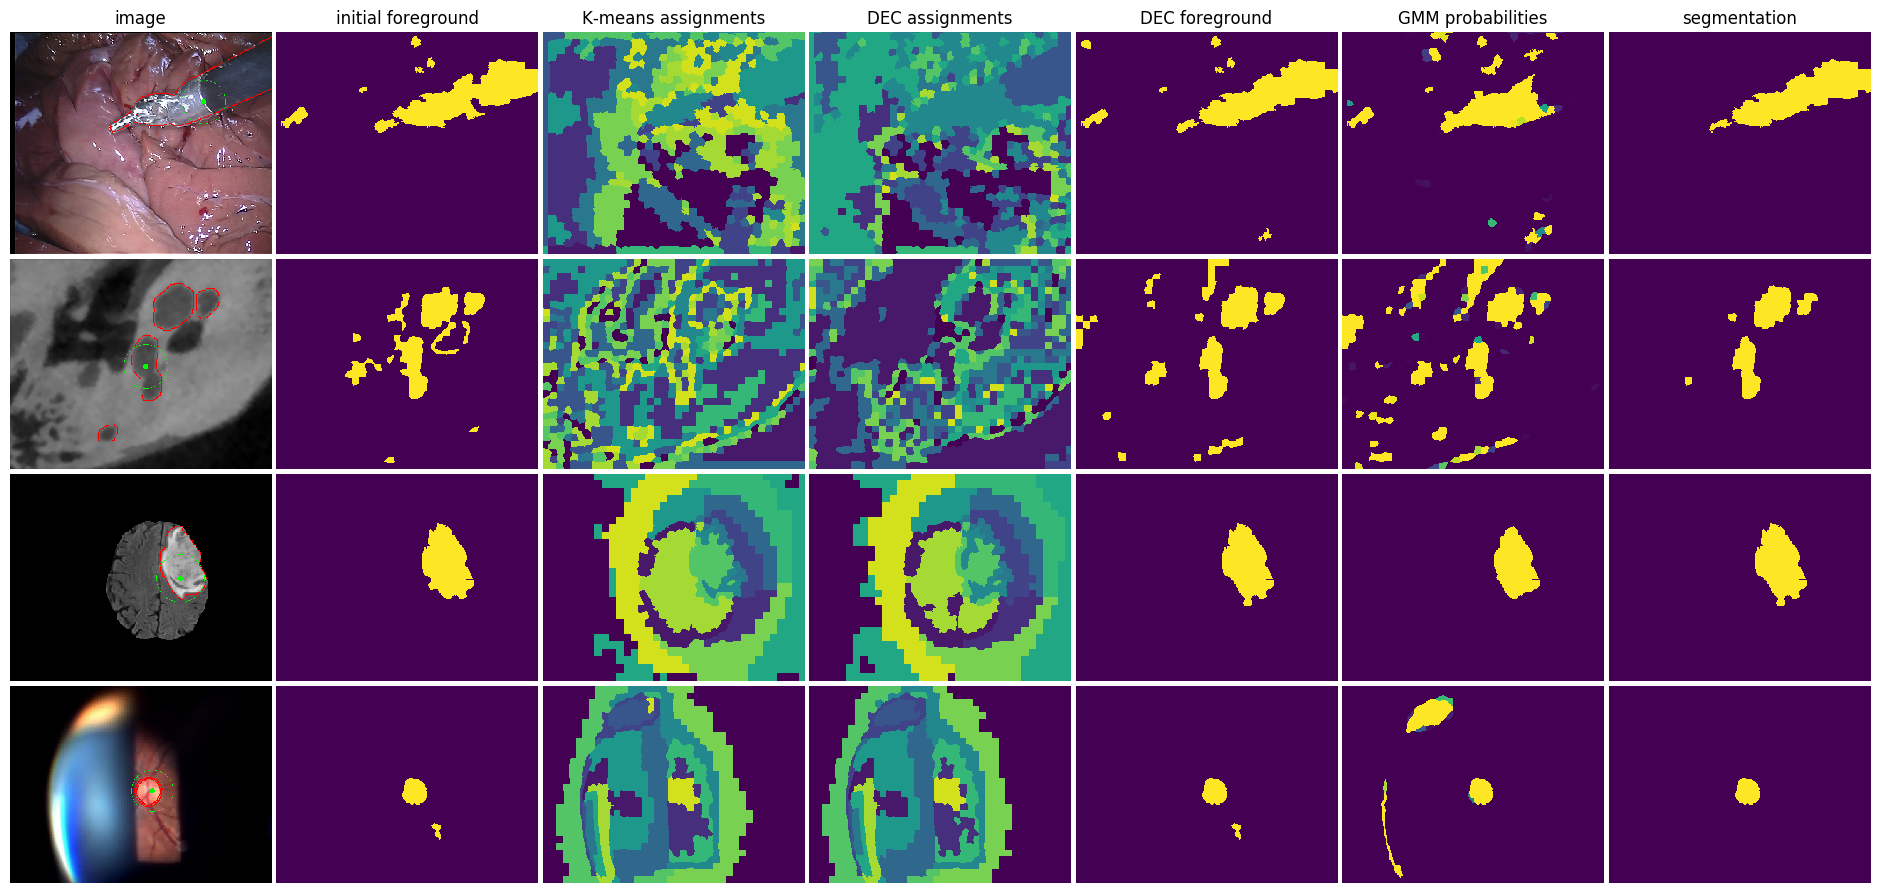
\includegraphics[width=0.99\textwidth]{prevs.png}
\caption{Example of objects of interest in different video and volumetric modalities. Each type contains 4 sequences. We show a single frame per sequence.
  From top to bottom: Tweezer, Cochlea, Slitlamp, and Brain}
\label{fig:dset_previews}
\end{figure}

\section{Annotation Software and Web Platform}
In the frame of this thesis, a flexible and elegant annotation software was developed that supports as pointing device a traditional mouse, a pen compatible with touch-screens, as well as an interface to connect a eye-gaze tracker through the USB port.
Also, a web interface was designed and implemented that allows a user to upload a sequence annotated using the above software, and download the generated pixel-wise segmentation when they are ready.
We now describe both contributions.

\subsection{Sequence annotation tool}
\label{sec:anna}

The typical annotation workflow is as follows:

\begin{enumerate}
  \item[-]{Provide as input a volume/video. These can be either DICOM \cite{dicom}, or video files.}
  \item[-]{Optional: Set the framerate at which the sequence will play (right knob on Fig. \ref{fig:anna}).}
  \item[-]{Optional: Connect the software to the eye-gaze tracker server. The tracker will then act as a secondary mouse.}
  \item[-]{Hit the play button. The sequence unfolds.}
  \item[-]{Give point annotations:}
    \begin{itemize}
      \item[-]{When using mouse: Simply click on the desired region.}
      \item[-]{When using gaze-tracker: Place gaze on region and use right button (Fig. \ref{fig:anna}) to activate the recording of locations.}
    \end{itemize}
  \item[-]{Save locations in \gls{csv} file.}
\end{enumerate}

\begin{figure}[!htpb]
  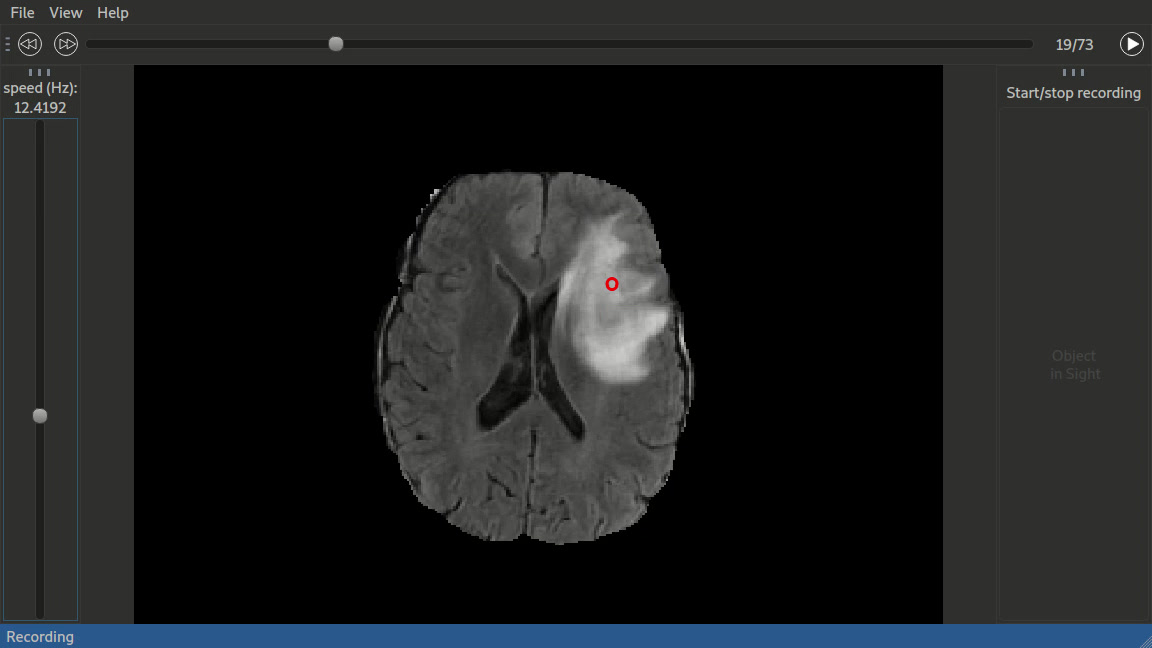
\includegraphics[width=0.99\textwidth]{anna0.png}
  \caption{Screenshot of annotation tool. }
  \label{fig:anna}
\end{figure}

The software is intended to be cross-platform and be compatible with a variety of input formats.
Second, as our early experiments relied on an eye-gaze tracker, our software needed to be compatible with the proprietary backend given by the manufacturer.
Third, a simple \gls{gui} was needed to display images and allow the user to select his favorite modality of annotation.
The latter requirements drove our choice towards the Qt5 framework \cite{eng16}, which relies on C++ and provides convenient widgets out of the box.
Our software supports allows to annotate using a mouse and an eye-gaze tracker \cite{eyetribe}.
As platform, it supports the Linux, MacOS and Windows operating systems.
We provide the source code at \href{https://github.com/aimi-lab/Anna}.

\subsection{Web platform}
The segmentation methods presented in the next chapters require important computational resources, namely a \gls{gpu} to train deep networks.
We therefore provide a way for users to upload their data along with the corresponding 2D locations to a server that will perform the necessary computations remotely and send back segmentation results when they are available.
Concretely, we develop a web interface that provides:

\begin{itemize}
  \item[-]{Links to download the annotation software (Sec. \ref{sec:anna}).}
  \item[-]{A login mechanism that provides us with a contact e-mail address.}
  \item[-]{An upload form where the user drops his sequence along with the 2D locations}
\end{itemize}

Once the data has been uploaded, a task object is created and queued until computational resources are available.
After completion, the user is warned that he can download his segmentations via a URL.

\begin{figure}[!htpb]
  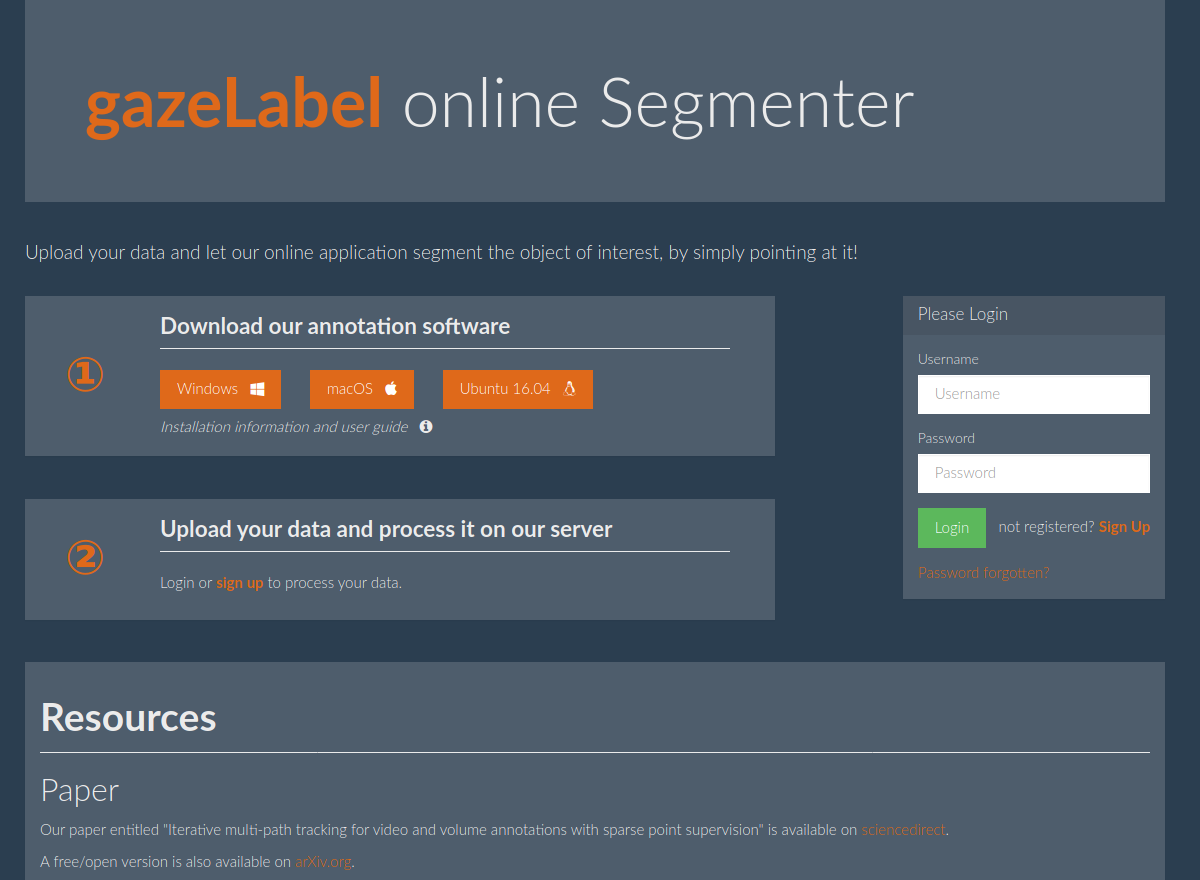
\includegraphics[width=0.99\textwidth]{gazelabel.png}
  \caption{Screenshot of our web platform. Home page.}
  \label{fig:anna}
\end{figure}

The frontend, which generates the web pages uses the \href{https://webpack.js.org}{Webpack} bundler.
The backend is based on the \href{https://www.djangoproject.com/}{Django} framework, which handles different applications, namely the forms (login, data upload), the job queue, and the database.

\begin{figure}[!htpb]
  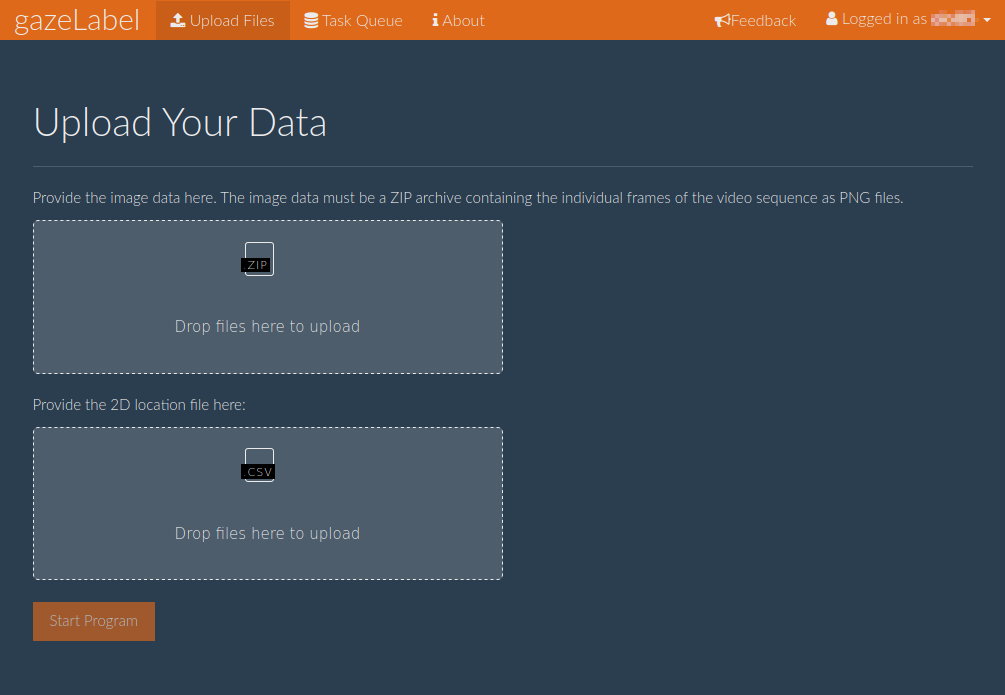
\includegraphics[width=0.99\textwidth]{gazelabel_upload.png}
  \caption{Screenshot of our web platform, where the user can upload a sequence and its corresponding annotations. The task queue panel shows the state of the submitted tasks.}
  \label{fig:anna_upload}
\end{figure}



\section{Related Works}

Past research that address this issue can be roughly divided in two categories,
where the first leverages computer vision techniques to generate segmentation masks from sparse and/or noisy annotations, while the second focuses on developping Machine Learning techniques to minimize an annotation budget.
In practice, both categories often overlap.

We start by giving an overview of state-of-the-art in computer vision.
Next, we focus on \gls{ml} methods.
In particular, we emphasize on domains that target segmentation in a semi-supervised setting.

\subsection{Computer Vision Methods}
Another line of research focuses on the annotation protocol itself so as to complement the above efforts.
While the most tedious protocol requires that images be manually segmented at a pixel-level, many computer-vision approaches exist to facilitate this task.

Early contributions relied on the Active Contour model \cite{kass88}, which assumes that an initial contour is given and parameterized as the nodes of a spline curve, in this context called an elastic snake.
The segmentation problem is formulated as finding the deformation of the initial snake that minimizes an energy term.
In its simplest form, the energy term is composed of a term that determines the fitting of the snake to the edges of the image, while another term controls the smoothness of the snake.
The energy is then minimized using gradient descent.
Following works alleviate the problem of robustness brought by noisy edge maps by minimizing the Mumford-Shah functional \cite{chan01}, and parameterize the contour using the level-set method \cite{osher88}.

More recently, annotations in the form of scribbles were considered, where the annotator is asked to draw crude delineations of one or several objects of interest, along with a scribble on the background.
A first method that handles such kind of annotations relies on the Random-Walk algorithm \cite{grady06}.
The segmentation problem reduces to assigning to each unlabeled pixel a random-walker. The label of the latter pixel is then determined by the finding the label for which the walker has a maximum probability of reaching first.

Relying on the same annotation requirement, the graph-cut approach \cite{Boykov2006}
minimizes an Markov Random Field energy objective that considers unary terms (a scalar on each pixel), and a pairwise term that models the similarity of neighboring pixels.
Concretely, the image or volume is represented as a region adjacency graph where each pixel is assigned a node, and edges connect adjacent pixels.
Each annotated positive pixels is connected to a source node, while annotated negatives are connected to a sink node.
The energy minimization is then performed using the min-cut/max-flow algorithm \cite{goldberg88}.
Using the same algorithm, grab-cut \cite{rother04}, further simplifies the scribble-based annotation protocol by considering bounding-boxes around the object of interest, which provide crude labels on both foreground and background in a single stroke.

Along the same line, \cite{criminisi08}

\subsection{On the Wise Use of Annotation Budget}
The problem of scarcity of labeled data can also be posed in the following manner:
Given a limited annotation budget, i.e. when only a few hours of annotation work can be provided, how can one make the best use of it?

\gls{al} \cite{settles09} considers semi-supervised learning scenarios, where abundant unlabeled data are available.
\gls{al} algorithms select unlabeled samples that are the most informative to the \gls{ml} model, i.e. it assumes that many unlabeled samples represent redundant information to the late-stage \gls{ml} model.
In \cite{KonSznFua15}, authors devise a strategy to select unlabeled supervoxels of a 3D volume so as to segment volumes of various modalities.
The approach iteratively trains a classifier and takes its entropy as measure of uncertainty.
Combining the latter with a geometric prior, which takes into account intuitive rules on spatial coherence, they sample a batch of most uncertain samples.
The classifier is then re-trained using the newly annotated samples.

Crowd-sourcing, refers to the outsourcing of the annotation task to a high number of annotators \cite{orting19}.
Its use in the frame of medical imaging poses several limitations.
First, the difficulty of the annotation task can prohibit the effective use of crowd-sourcing, e.g when the structure of interest is hard to distinguish \cite{orting19}.
Another limitation is the nature of the data, i.e. one usually prefers to pre-classify brain scans and submit to workers the slices where tumors are present.
Last, one must usually integrate a test-task to ensure the competence of workers, or filter-out annotations provided by ``poorly performing'' workers \cite{park18}.

\subsection{Transfer Learning, Semi-supervised Learning, and Domain Adaptation}
\gls{tl} consists in using a \gls{ml} model trained for the task of interest, but using a training set of different nature than the targeted domain, e.g. train a \gls{cnn} to segment natural objects (trees, cars, ...) for the segmentation of surgical tools.
As pointed out by \cite{oliver18}, an important and implicit assumption in that context is that both datasets share similar data distributions.

\gls{ssl} is a broad category of \gls{ml} algorithm that combines traditional supervised learning tasks, where a fully labeled training dataset is available, along with an abundant unlabeled dataset.
The latter can, under specific conditions, boost the performance of an \gls{ml} model trained with labeled dataset only, i.e. in a fully-supervised manner.
The basic idea is that the ML model may acquire knowledge of the data distribution from the unlabeled set.
Here again, one assumes that both data domains share similar distributions.
In \cite{ghafoorian17}, authors show experimentally that a \gls{nn} trained to segment tumors on MRI brain scans acquired in a given MRI protocol, perform poorly when transfered to another protocol, as the shape, intensities, and contrast level are inconsistent.

\gls{da} addresses the problem of adapting the model so as to take into account domain shift, i.e. the discrepancies between the training and target domain.
In \cite{perone19}, authors devise a strategy to segment MRI scans of spinal cords using a model trained with images taken at a specific field-of-view, and transfer to another field-of-view in an unsupervised fashion.
Their approach leverages data-augmentation to enforce a consistency between the augmented and pristine images of the unlabeled set, while jointly training with the labeled set with traditional cross-entropy loss.
On the same image modality, \cite{li20} resort to adversarial training. They jointly train a segmentation model and a discriminator wit shared weights. The discriminator is trained to discriminate between the source and target domain.





%%% Local Variables:
%%% mode: latex
%%% TeX-master: "../../main"
%%% End:

\resetfigpath{2-eel}

\chapter{Expected exponential loss for gaze-based video and volume}
\label{eel} % For referencing the chapter elsewhere, use \ref{Chapter1}

\section{Notation}
Let an image sequence (or volume) be denoted $\mathcal{I} = [I_{0}, \cdots , I_{T}]$ and let $\mathcal{G} = \{g_{t} \}^{T}_{t=0}$ such that $g_t\in \mathbb{R}^{2}$ is a 2D gaze pixel location in $I_{t}$.

While we ideally would like
a pixel-wise segmentation, we choose to decompose each image using a temporal superpixel
strategy \cite{chang13} and operate at a superpixel level instead.

We thus let $I_t$ be described by the set of non-overlapping superpixels
$S_{t} = \{S^{n}_t\}^{N_t}_{n=0}$ and define the set of all superpixels across all
images as $\mathcal{S} = \{S_t \}^{T}_{t=0}$.
We denote the set $\mathcal{P} = \{S^{n}_t | g_{t} \subset S^{n}_t, t = 0, \cdots, T, n = 0, \cdots, N_t \}$ as all
superpixels observed and the rest as $\mathcal{U} = \mathcal{S} \backslash \mathcal{P}$.
We associate with each $S^{n}_t$ a binary random variable $Y^{n}_{t} \in \{-1, 1\} = \mathcal{Y}$,
such that $Y^{n}_t = 1$ if $S^{n}_t$ is part of the object and -1 otherwise.
In particular, we defined $Y_n$ as a Bernoulli random variable, $Y^{n}_t \sim Ber(\epsilon_{S^{n}_{t}})$, $\epsilon \in (0,1)$.
Note that for positive superpixels $S^{n}_t \in \mathcal{P}$, we consider these as part of the object and let $Y^{n}_t = 1$ with $\epsilon_{S^{n}_{t}}=1$.

\section{Method}
Our goal is to train a prediction function, $f : S \rightarrow Y$
that takes into account observed superpixels as well as the unobserved ones.
To do this we propose the following Expected Exponential Loss (EEL) function:

\begin{equation}
  \mathcal{L}_{EEL} = \mathbb{E}^{Y} \left[ \sum_{S \in \{ \mathcal{P}, \mathcal{U}\}} e^{-f(S)Y}\right]
\end{equation}

where the expectation is taken with respect to all $Y$s.
By linearity of expectation and the fact that labeled superpixels have no uncertainty in their label, we can rewrite the loss for all superpixels as

\begin{equation}
  \label{eq:eel}
  \mathcal{L}_{EEL} = \sum_{S \in \mathcal{P}} e^{-f(S)} + \left( \sum_{S \in \{ \mathcal{P}} \epsilon_{S} e^{-f(S)Y} + (1-\epsilon_{S}) e^{f(S)Y}\right)
\end{equation}

Note that Eq. \ref{eq:eel} is a generalization of the Exponential Loss (EL) \cite{hastie09}.
In the case where labels are known, the loss is the same as the traditional loss as the expectation is superfluous.
For unknown samples, the value of $\epsilon_{S}$ weighs the impact of the superpixels.
For instance, if $\epsilon_{S}$ is close to 0.5, the sample does not affect the loss.
Conversely values of $\epsilon_{S}$ close to 1 (or 0) will strongly impact the loss.

\section{Implementation}
We implemented the above EEL within a traditional Gradient Boosting classifier \cite{hastie09},
by regressing to the residual given by the derivate of Eq. \ref{eq:eel}.
For all experiments, we used stumps as weak learners, a shrinkage factor of 1 and the line search was replaced by a constant weight of 1.
The weak learner stumps operate on features extracted from the center of the superpixel.
In particular, we used generic Overfeat features \cite{sermanet13} which provide a rich
characterization of a region and its context (e.g. 4086 sized feature vector).
During training we used all superpixels in $\mathcal{P}$ and used $10\%$ of those in U.
A total of 50 boosting rounds was performed in all cases.
To predict segmentations for the entire volume, we
predicted the remaining $90\%$ of superpixels in $\mathcal{U}$.

\section{Probability estimation for unknown labels}
\label{sec:eel_estim}
To estimate $\epsilon_{S}$ in Eq. \ref{eq:eel}, we take inspiration from the Label Propagation method \cite{zhou04}, which uses a limited number of positive and negative samples to iteratively propagate labels to unobserved samples.
In our setting however, we only propagate positive samples to unlabeled
samples using the gaze information as well as pixel motion estimation to constrain the probability diffusion.
We let $P_{0} = \left[p_0,\cdots, p_{N}\right]$ be a vector of initial probabilities for all superpixels in a given image, where $p_n = P(Y = 1|\mathcal{P})$ is the probability that superpixel $S_{n}$ is part of the object.
In practice, we estimate $p_{n}$ by computing a gaze dependent Lab color model using all gaze
locations and assessing how likely a superpixel $S_{n}$ is part of the object.
That is, we compute

\begin{equation}
  p_{n} = \max_{S \in \mathcal{P}} \mathcal{N}(S_{n}|\mu_{s},\Sigma_{S})
  \end{equation}

  where $\mathcal{N}$ is a Gaussian distribution such that $\mu_{S}$ and $\Sigma_{S}$ are the color mean and covariance of pixels in a positive superpixel $S$.
  Also, we fix $p_{n}=1$ for positive superpixels.
  To propagate probabilities, we also define a $N \times N$ affinity matrix, denoted W
with values

\begin{equation}
w_{ij} = exp(-||\theta_{i} - \theta_{j}||^2 / 2\sigma_{a}^{2}) exp(-||C(S_i) - C(S_j)||^2 / 2\sigma_{d}^{2})
\end{equation}

where for superpixel $S_{i}$, $C(S_{i})$ is its center and $\theta_{i}$ is its average gradient orientation.
In cases where $S_{i}$ and $S_{j}$ are separated by more than $\tau$ pixels, $w_{ij}=0$.
$\sigma_{a}$ and $\sigma_{d}$ are model parameters reflecting the variance in angle difference and the impact of neighboring superpixels, respectively.

Propagation can the be computed iteratively by solving

\begin{equation}
P_{m+1} = \alpha \Omega P_{m} + (1 - \alpha)P_{0}
\end{equation}

where $\alpha \in (0,1)$ is a diffusion parameter, $D$ is a diagonal matrix with entries $d_{ii}=\sum_{j}w_{ij}$ and $\Omega = D^{-1/2} W D^{-1/2}$.

Fig. \ref{fig:eel_propagation} shows the initial $P_{0}$, the associated optical flow regions and the final propagated probability for a given image.
While the original method described in \cite{zhou04} hinged on a minimum of one positive and one negative sample to prove the existence of a closed form convergence solution, the same cannot be said of the current setting where no negative samples are known.
For this reason, we iterate a total of $10$ times and then use the estimates for the $\epsilon_{S}$
values in Eq. \ref{eq:eel}.
This value was experimentally determined and shown to perform well for a
number of image sequences (see Sec. \ref{sec:eel_exp}).
The process is repeated for all frames in the sequence.

Note that the probability estimate is computed from a single gaze sequence and the corre-
sponding image data. As such, if more than one domain expert viewed the same sequence, as it
is the case in Crowd-Sourcing tasks, this process can be repeated for each observer and averaged
over all observers.
In our experiments, we show that doing so brings increased performances over that given by a single observer.

\section{Experiments}
\label{sec:eel_exp}
To evaluate the performance of our method we compare it to the method presented in \cite{vilarino07}.
We also show how the EEL approach compares with that of using $\epsilon_{S}$ estimates only
(see Sec. \ref{sec:eel_estim}), as well using $\epsilon_{S}$, with a traditional EL when binarizing the labels using a fixed
threshold $\epsilon_{S}=0.5$.
The following parameters were kept constant: $\alpha=0.95$, $\sigma_{a}=0.5$, $\sigma_{d}=50$, $\tau = 50$ and the superpixel size was set to match $1°$ on the viewing monitor.
We evaluated each of the above mentioned methods on 4 very different image sequences (see
Fig. 1 for examples)

\begin{enumerate}
\item A 3D brain MRI containing a tumor to annotate from the BRATS
challenge \cite{BRATSChall} consisting of 73 slices
\item A 30 frame surgical video sequence from the MICCAI
EndoVision challenge \cite{endochal} where a surgical instrument must be annotated
\item A 95-slice 3D CT scan where a cochlea must be annotated and
\item A slit-lamp video recording (195 frames) of a human retina where the optic disk must be segmented.
\end{enumerate}

Pixel-wise annotated ground truth
on all frames of each sequence was either available or produced by a domain expert.
In all sequences, one and only one object is present throughout the sequence.
Our method was implemented in MATLAB and takes roughly 30 minutes to segment a
30 frame volume with $720 \times 576$ sized frames, of which the bulk of time is used to compute
temporal superpixels and training our classifier.
Even though real-time requirements are not necessary in this application, we believe this computation time could be reduced with an improved implementation.
Gaze locations were collected with an Eye Tribe Tracker (Copenhagen, Denmark) which provide
$1°$ tracking accuracy.
To collect gaze locations, a computer monitor and the tracker
was placed roughly 1 meter from the experts face.
Device-specific calibration was performed before all recordings (i.e. a 2-minute long procedure done once before each viewing).
2D gaze locations were collected and mapped to the viewed image content using the manufacturers API.
Domain experts were instructed to stare at the target and avoid looking at non-object image
regions.
Once each sequence was observed, the different methods inferred the object throughout
the entire image data.

\section{Results}
\subsection{Annotation accuracy}
Table 1 reports the Area Under the Curve (AUC) and the F1 score performances of each method applied to each dataset.
In general, we report that the proposed combined label estimation and EEL function provide the highest AUC and F1 score values across the tested sequences.
Fig. \ref{fig:eel_qual_res} visually depicts example frames from each sequence and the outcome of each method, as well as the ground truth.

To generate these binary images, a $5\%$ false positive threshold was applied (i.e. threshold was determined using the ground truth).
One can see that in cases where the object to segment occupies large areas of the image,
as is the case for the surgical instrument, both the traditional loss approach and that of \cite{vilarino07} do not perform as well since they treat significant portions of the background as positive samples during their respective learning phases.
\begin{figure}
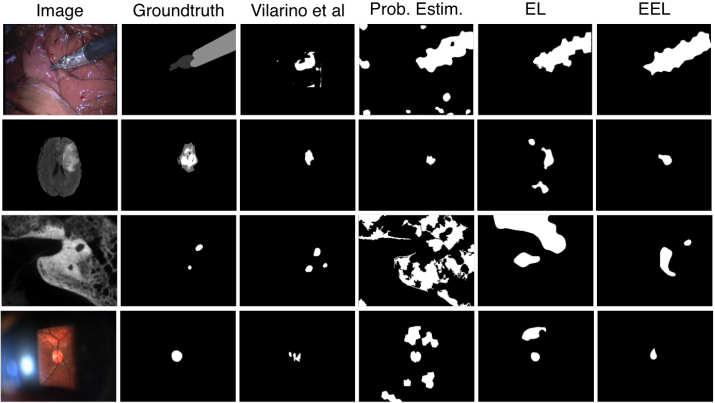
\includegraphics[width=0.99\textwidth]{qual_results}
\caption{Qualitative results. Each row shows a different dataset with an example image,
the associated desired ground truth and the produced outcome of \cite{vilarino07}, using the probability
estimation approach, EL approach and the proposed EEL.
Binary images were generated by thresholding results at a $5\%$ False Positive Rate.}
\label{fig:eel_qual_res}
\end{figure}

\subsection{Gaze variance}
In order to estimate the variance in annotations obtained with our strategy, $7$ gaze observations were performed on the same laparoscopic image sequence.
From these gaze observations, we ran our method on each set independently.
Fig. 5(left) shows the average ROC curve and standard error associated with our approach.
In addition, we show similar performances when using the EL and when using the estimated labels only.
On average we see that the EL does no better than the label estimation process, while the label estimation approach has slightly less variability.
Overall, the EEL approach not only outperforms the other settings, but has lower variance as well.

\subsection{Crowd-sourcing context}
From the 7 gaze observations collected, we consider a Crowd-Sourcing context where the label estimation is combined as described in Sec. \ref{sec:eel_estim} in order to generate the associated ground truth.
Fig. 5(right) illustrates the performance attained when doing so.
While the overall trend is no different to the previous experiment, the performance reached by the EEL approach is vastly higher.
This is unsurprising given that more gaze information is provided in this setting (i.e. 7 annotators) and that more of the object is in fact
viewed, yielding thus more positive samples, as well as better $\epsilon_{S}$ estimates.

\begin{figure}
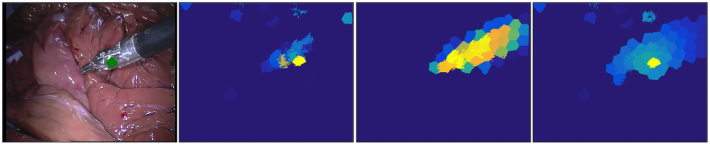
\includegraphics[width=0.99\textwidth]{propagation}
\caption{Probability propagation. Left to right: original image with the gaze location high-
lighted in green; Initial $P_{0}$ estimate from the gaze-based color model; Image regions with high
optical flow; Estimated probability after propagation. Dark blue regions depict low probability
while warmer regions correspond to higher probabilities.}
\label{fig:eel_propagation}
\end{figure}

\section{Conclusion}
In this work we have presented a strategy for domain experts to provide useful pixel-wise
annotations in a passive way. By leveraging cheap eye gaze tracking technology, we have showed
that gaze information can be used to produce segmentation ground truth in a variety of 3D
or video imaging modalities. We achieved this by introducing a novel EEL function that is
robust to large amounts of unlabeled data and few positive samples. We also demonstrated
that our approach could be used in the context of crowd-sourcing where multiple annotators
are available.
While this work presents an initial attempt, a number of aspects of this work need to
be explored moving forward. In particular, we plan to tackle the case when the object is not
present during the entire sequence, as well as cases where multiple objects are present. Naturally,
asking more of the user would provide additional information, but our goal is to keep this to a
minimum. For this reason, we also plan on determining how our method could work with noisy
object observations, as $100\%$ compliant users may not always be possible.
%%% Local Variables:
%%% mode: latex
%%% TeX-master: "../../main"
%%% End:

% \chapter{Feature Extraction}
\label{ch:methods}
This chapter first describes the dataset modalities and properties. Second, we give an overview of our pipeline from training to evaluation. Third, we introduce the proposed methods for feature learning as well as the evaluation scheme. Concerning the feature representation learning, we first introduce our baseline methods, followed by the U-Net based methods.

Tab. \ref{tab:dataset_stat} summarizes the 13 datasets. We used four different MRI brain sequences (A-D). To augment the number of images for one dataset, the last three datasets (B-D) are combined into one larger dataset \textit{MRI Brain (B-D)}. In a similar manner, dataset \textit{Slit-Lamp Retina (A-D)} is constructed from concatenating four independent datasets together. The two independent datasets of the inner ear CT could not be concatenated due to different image resolutions. To each dataset, we also have corresponding xy-coordinates of the gaze location.

\begin{table}[ht]
   \centering
   \caption[Dataset statistics]{Summary and statistics of used datasets. Note the variety in size, resolution and color space.}
   \begin{tabular}{l|c|c|c|c|c}
      \toprule
      \textbf{Name} & \textbf{Size $N$} & \textbf{Height $H$ [px]} & \textbf{Width $W$ [px]} & \textbf{\#Channels $C$} \\
      \midrule
      Surgical Video Sequence & 1125 & 576 & 720 & 3 - RGB \\
      \midrule
      MRI Brain A & 129 & 540 & 782 & 1 - Gray \\
      MRI Brain B & 69 & 512 & 680 & 1 - Gray \\
      MRI Brain C & 75 & 512 & 680 & 1 - Gray \\
      MRI Brain D & 75 & 512 & 680 & 1 - Gray \\
      MRI Brain (B-D) & 219 & 512 & 680 & 1 - Gray \\
      \midrule
      CT Inner Ear A & 96 & 191 & 252 & 1 - Gray \\
      CT Inner Ear B & 99 & 290 & 300 & 1 - Gray \\
      \midrule
      Slit-Lamp Retina A & 194 & 512 & 680 & 3 - RGB \\
      Slit-Lamp Retina B & 121 & 512 & 680 & 3 - RGB \\
      Slit-Lamp Retina C & 75 & 512 & 680 & 3 - RGB \\
      Slit-Lamp Retina D & 130 & 512 & 680 & 3 - RGB \\
      Slit-Lamp Retina (A-D) & 520 & 512 & 680 & 3 - RGB \\
      \bottomrule
   \end{tabular}
   \label{tab:dataset_stat}
\end{table}

\section{Framework} \label{framework}
Fig. \ref{fig:Framework} illustrates our feature learning and evaluation framework. The individual blocks, such as superpixel segmentation, feature learning methods, and evaluation method, are elaborated in subsequent chapters. 

\begin{figure}[!htpb]
  \centering
  \includegraphics[width=13cm]{framework/framework}
  \caption[Framework description]{Framework description and how the individual parts are connected. Out of image data, superpixel segmentation and possible gaze locations, the feature learning algorithm construct a feature matrix $\boldsymbol{X}$, describing each superpixel by a feature. A Random Forest binary classifier is then trained and validated to make predictions of every superpixel. The labels are denoted by $\boldsymbol{y}$, describing if a superpixel belongs to foreground or background. At the bottom-right, we measure the performance of the classifier.}
  \label{fig:Framework}
\end{figure}

Performance evaluation of the different feature learning methods is done on a superpixel level. Hence, the feature learning methods shall output a feature vector for each of the superpixels. Refer to chapter \ref{superpixel_segm} for more details about the superpixel segmentation.

Let $N$ be the number of images in a data sequence and $S$ the number of superpixels over all sequence. As an example, if we have exactly $200$ superpixels per image, we would have $S=N \cdot 200$ superpixels in that sequence. To every superpixel, we want to assign a feature vector of dimension $D$. We can write the sequence feature matrix as $\boldsymbol{X} = [\boldsymbol{x}_1,...,\boldsymbol{x}_S]^T \in \mathbb{R}^{S \times D}$. Let $\boldsymbol{y} = [y_1,...y_S]^T \in \{0,1\}^S$ be the labels, meaning that $y_i=1$ for superpixels that count to the object of interest and $y_i=0$ for superpixels belonging to the background. Using the feature matrix $\boldsymbol{X}$ and the label vector $\boldsymbol{y}$, a random forest classifier then calculates performance measures, such as Precision-Recall curve and \textit{max F1-Score}. How the Random Forest classifier is applied is described in chapter \ref{random_forest}.

Some feature learning methods use the gaze location as an object prior, given as xy-coordinates for each image frame. The green point in Fig. \ref{fig:Framework} illustrates this location.

\section{Superpixel Segmentation} \label{superpixel_segm}
As described above, the performance evaluation is performed on a superpixel level. Having a feature vector for each superpixel instead of each pixel reduces the computational requirements. 

We used the superpixel segmentation algorithm ASLIC developed by Achanta et al. \cite{achanta12}.
SLIC stands for \textit{simple linear iterative clustering} and ASLIC for \textit{adaptive} SLIC. It relies on k-means clustering performed in color and spatial space. A trade-off between color similarity and spatial proximity is found necessary. In the SLIC approach, the problem is solved by using a compactness parameter. For images with both, flat and very textured regions, using the same compactness parameter lead to smooth regular-sized superpixel in the flat regions and highly irregular sized superpixel in textured regions. Thus, Achanta et al. invented the ASLIC approach, which adaptively chooses the compactness parameter for each superpixel differently. Fig. \ref{fig:ExSuperpixel} shows an example of using ASLIC on dataset \textit{Slit-Lamp Retina A}.

\begin{figure}[!htbp]
  \centering
  \label{fig:subfig:example_superpixel}
  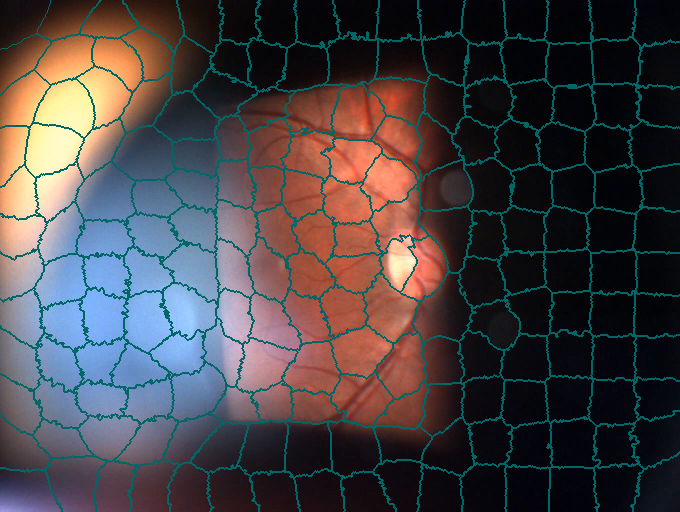
\includegraphics[width=3.5cm]{superpixel_examples/ds12_superpixel}
  \caption[Example of superpixel segmentation]{Example of ASLIC superpixel segmentation on dataset \textit{Slit-Lamp Retina A} with number of superpixels $S=200$. Note the regular shape of superpixels in all regions.}
  \label{fig:ExSuperpixel}
\end{figure}

As parameter, the number of superpixels is crucial. In terms of trade-off, setting a large value will capture the contours of objects more accurately, at the cost of having a higher quantity of samples to predict/classify. We verified that taking $200$ superpixels per frame produces reasonably good segmentation on all our sequences.

Having at disposal ground truth data at pixel-level, we set the values of the output variable $\boldsymbol{y}$ the following way.
If one superpixel is covered by the ground truth pixel-wise segmentation by more than $50\%$ of its area, this specific superpixel is assigned to the foreground. Otherwise, it is assigned to the background.

\section{Feature Learning: Baselines} \label{ch:baselines}
To evaluate the performance of a method, a standard approach is to compare it to baseline methods. We used three different methods as baselines. The first method is called \textit{Bag of Visual Words (BoVW)}. A variant of the \textit{BoVW} approach is presented in a second baseline approach, so called \textit{Sparse Coded Spatial Pyramid (ScSP)}. This method is currently used in the superordinate project and therefore of high importance. The last baseline method follows the idea of transfer learning and uses a pre-trained VGG-16 network.

\subsection{Bag of Visual Words} \label{bow}
\begingroup
\setlength\intextsep{0pt}
\begin{wrapfigure}[4]{l}[0pt]{1.4cm}

\includegraphics[height=1.5cm]{icons/bovw}
\end{wrapfigure}

Bag of Visual Words (\textit{BoVW}), or Bag of Visual Features, is an unsupervised feature encoding method successfully utilized in scene classification \cite{zhang15}.
The algorithm can be split into feature learning and feature encoding phase \cite{cheriyadat14}. Feature learning phase is illustrated in Fig. \ref{fig:subfig:bow_training}. We developed a \textit{BoVW} approach where we choose the keypoints randomly over all images in a dataset. Each keypoint is then described by a SIFT descriptor of dimension 128. Subsequently, k-means vector quantization quantizes the keypoint descriptors into $K$ classes. Let $\boldsymbol{F} = [\boldsymbol{f}_1,...,\boldsymbol{f}_M]^T \in \mathbb{R}^{M \times 128}$ be the SIFT appearance descriptor of the $M$ keypoints. Eq. \ref{eq:k_means} describes the k-means objective function, where $\boldsymbol{C} = [\boldsymbol{c}_1,...,\boldsymbol{c}_K]^T \in \mathbb{R}^{K \times 128}$ denotes the codebook.

\endgroup

\begin{equation}
   \min_{\boldsymbol{C}} \sum_{m=1}^M \min_{k=1...K} \|\boldsymbol{f}_m - \boldsymbol{c}_k\|^2
   \label{eq:k_means} 
\end{equation}
\vspace{6pt}

The coding phase, shown in Fig. \ref{fig:subfig:bow_coding}, consists of describing each pixel by a SIFT descriptor and assigning it to the class whose centroids is the closest in terms of Euclidean distance. Subsequently, the assigned classes of every pixel in one superpixel are described in a histogram of $K$ bins. This results in a feature matrix of all superpixels in a sequence being $\boldsymbol{X} = [\boldsymbol{x}_1,...,\boldsymbol{x}_S]^T \in \mathbb{R}^{S \times D}$, where $D = K$. Extraction of the SIFT descriptors is done on grayscale data.

For SIFT extraction we used the OpenCV \cite{openCV} package with Python interface and k-means vector quantization is performed using SciPy's \cite{scipy} clustering tools.

\begin{figure}[htbp]
  \centering
  \subfloat[BoVW feature learning phase]
  {
    \label{fig:subfig:bow_training}
    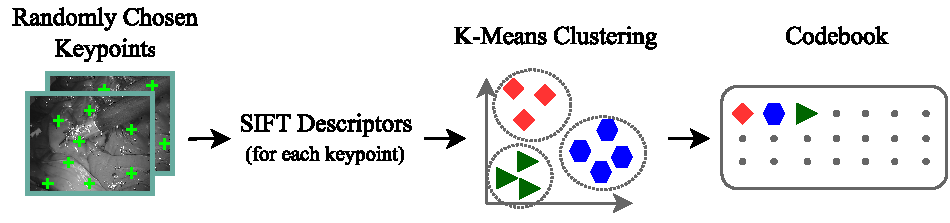
\includegraphics[width=10cm]{bovw/bow_approach_training}
  }
  \\
  \subfloat[BoVW feature encoding phase]
  {
    \label{fig:subfig:bow_coding}
    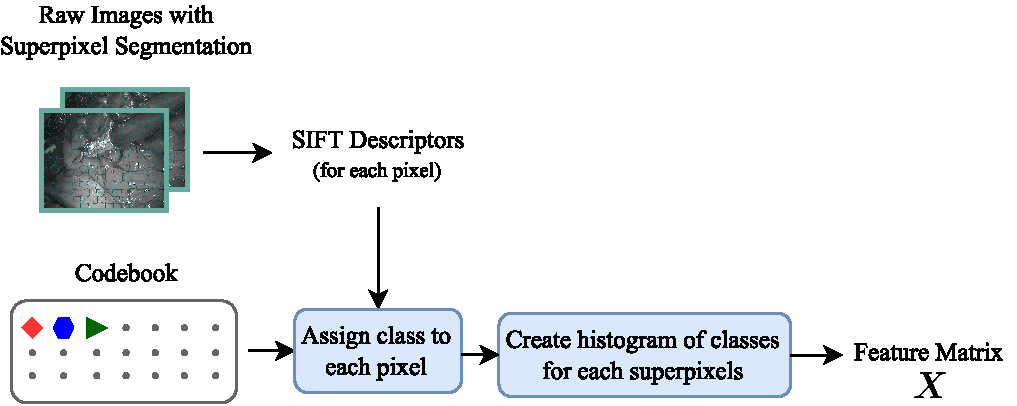
\includegraphics[width=11cm]{bovw/bow_approach_coding}
  }
  \caption[BoVW illustration]{Illustration of \textit{BoVW} approach, divided in two phases. (a) shows the feature learning phase, where SIFT descriptors of randomly chosen keypoints are quantized into a codebook. In the encoding phase (b), each pixel is described by a SIFT descriptor and assigned to a class using the codebook. Subsequently, for each superpixel, a histogram of all assigned classes is created, which makes up the final feature descriptor.}
  \label{fig:BoVW_approch}  
\end{figure}

\subsection{Sparse Coded Spatial Pyramid} \label{scp}
\begingroup
\setlength\intextsep{0pt}
\begin{wrapfigure}[4]{l}[0pt]{1.4cm}
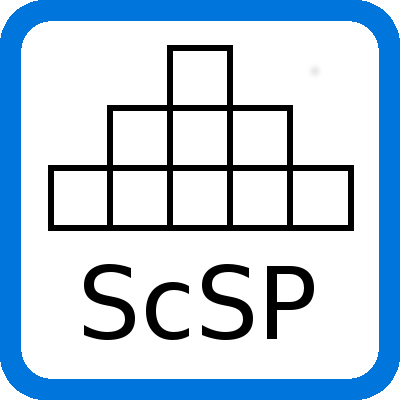
\includegraphics[height=1.5cm]{icons/scsp.png}
\end{wrapfigure}

Another baseline approach, called Sparse-coded Spatial Pyramid (\textit{ScSP}), can be seen as an improved version of the \textit{BoVW} approach with two main modifications. Firstly, instead of using standard k-means clustering, it uses sparse codes of SIFT features, and secondly, a pyramid representation is used. The following describes the added value of \textit{ScSP} with \textit{BoVW}.

\endgroup

%Max pooling instead of standard mean-statistics is not treated [well you just did it... cut and paste that somewhere relevant].

Mathematically, the objective of sparse coding for vector quantization can be written using matrix computation as shown in Eq. \ref{eq:sparse_codes}. The formulations below are adapted from Yang et al. \cite{yang09}.

\begin{samepage}
\begin{equation}
  \min_{\boldsymbol{U,C}} \sum_{m=1}^M \|\boldsymbol{f}_m - \boldsymbol{u}_m \boldsymbol{C}\|^2 + \lambda |\boldsymbol{u}_m|
  \label{eq:sparse_codes} 
\end{equation}
\begin{align*}
  \textrm{subject to } \|\boldsymbol{c}_k\| \leq 1, \hspace{6pt} \forall{k} = 1,2,...,K
\end{align*}
\end{samepage}

Similar to Eq. \ref{eq:k_means}, $\boldsymbol{f_m}$ represents the SIFT appearance vector of keypoint $m$ and $\boldsymbol{C}$ represents the codebook. $\boldsymbol{U} = [\boldsymbol{u}_1,...,\boldsymbol{u}_M]^T \in \mathbb{R}^{M \times K}$ defines the cluster membership indicator. The L2-norm on $\boldsymbol{c}_k$ is typically applied to avoid trivial solutions. If we drop the regularization term $\lambda |\boldsymbol{u}_m|$ and add a cardinality constraint to $\boldsymbol{u}_m$, meaning that only one element in $\boldsymbol{u}_m$ must be nonzero and positive, the sparse coding formulation in Eq. \ref{eq:sparse_codes} simplifies to k-means objective. Yang et al. \cite{yang09} approved that, compared to standard k-means coding, sparse coding can achieve a much lower reconstruction error due to less restrictive constraints. Sparsity also allows the representation to be specialized and capture salient properties of the image.

Lazebnik et al. \cite{lazebnik09} describe the spatial pyramid as a "collection of orderless feature histograms computed over cells defined by a multi-level recursive image decomposition". Fig. \ref{fig:pyramid_repr} show histograms extracted at different locations on an image. The final histogram representation is a concatenation of all histograms from all regions. After normalization, the concatenated histograms can again be seen as a histogram representing the full feature vector. Hence, for the example shown in Fig. \ref{fig:pyramid_repr} using pyramid levels $\boldsymbol{l} = [1,2,4]$, we have a feature dimension $D = K \cdot (1^2 + 2^2 + 4^2) = K \cdot 21$, where $K$ is the number of classes.

\begin{figure}[htbp]
  \centering
  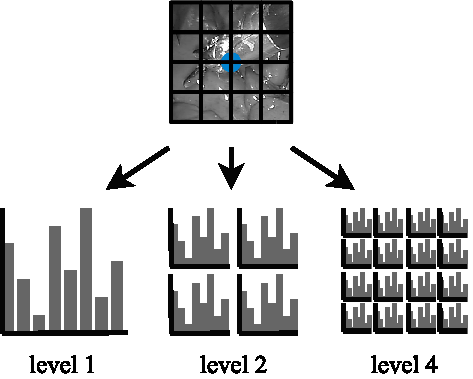
\includegraphics[width=6cm]{scp/pyramid_representation}
  \caption[Spatial pyramid representation]{Illustration of the spatial pyramid representation. Histograms are computed at different levels which are then concatenated into one big vector. After normalization, this vector can again be seen as a histogram vector.}
  \label{fig:pyramid_repr}
\end{figure}

Using a pyramid representation implies that the image patch needs to be square. Intuitively, one wants to enclose within the patch some visual context around the superpixel region. We refer to this parameter as patch size.
In practice, we train our codebook in a similar fashion to \textit{BoVW}, i.e. convert images to grayscale and randomly sample keypoints on every image of the sequence. Each keypoint then gives a SIFT feature vector. Once trained, we extract squared patches of dimension centered on each superpixel's centroid location. We used the implementation of \cite{imdescrip}.

\subsection{VGG-16 Pretrained} \label{vgg}
\begingroup
\setlength\intextsep{0pt}
\begin{wrapfigure}[4]{l}[0pt]{1.4cm}

\includegraphics[height=1.5cm]{icons/vgg.png}
\end{wrapfigure}

VGGNet is a CNN for large-scale image recognition proposed by Simonyan and Zisserman \cite{simonyan15}.
Their work was submitted to the ImageNet \cite{ILSVRC15} Challenge 2014 (ILSVRC-2014) where they secured the first and second places in the localization and classification task, respectively.
Transferring pre-trained VGGNets to other tasks has been successfully used by Long et al.
\cite{long15} in semantic segmentation and Ng et al. \cite{ng15} in emotion recognition. Those successes motivated us to evaluate the performance of using a pre-trained VGGNet. However, we did not follow any fine tuning steps.

\endgroup

Simonyan and Zisserman \cite{simonyan15} proposed various network models.
We used a model with 16 weight layers and $3 \times 3$ convolution strides, described as configuration D \cite[Tab. 1]{simonyan15}.
This model was trained on the ILSVRC-2014 dataset and weights are available online \cite{simonyan14a}.
We took advantage of an already existing implementation by F. Chollet in Keras \cite{Keras}.
Similar to the \textit{ScSP} approach, we extracted patches at superpixel centroids and fed it to the network.
Since the input dimension of the network is fixed ($244 \times 244 \times 3$), our input data needed to be scaled to that size.
Resizing is done using bicubic interpolation method of Python's SciPy \cite{scipy} package.
The features are then extracted from the penultimate fully-connected layer, resulting in a feature dimension of $D=4096$.

From a theoretical point of view, let us mention that most machine learning methods make the assumption that training and unseen data lie in the same feature space and have a similar distribution.
However, in many real-world applications, this assumption may not hold, as stated by Pan et al. \cite{pan2010}.
In a setup where the training data largely differs (in the latter sense) from the data used for prediction, we talk about "Transfer Learning". We assume that a network pre-trained on a very large-scale dataset with high generalization will produce good features for our task.

\section{Feature Learning: U-Net Based} \label{ch:unet_based}
We now describe our U-Net based feature extraction methods. We first explain the architecture of the "core" model, i.e. one that will be modified to account for different outputs and loss functions. We dedicate the second section to data augmentation. The third section describes how the features can be extracted from the CNN model to obtain feature vectors. Our various modified U-Nets will then be described in detail. Finally, an overview summarizes all U-Net based methods.

\subsection{Core Model} \label{model}
Our CNN is a slight modification of the original U-Net structure described in chapter \ref{u_net}. We did not use the U-Net for image segmentation, as initially done by Ronneberger et. al. Instead, we trained the network in an unsupervised manner, like an autoencoder, on our data and extracted features at the lowest level. Some of our methods operate in a weakly-supervised fashion, where information related to the gaze location is used as a prior.

Fig. \ref{fig:unet_model} shows a modified U-Net structure. Similar to the original structure, we used two stacked convolution layers with $3 \times 3$ filter size and stride $1$ per level. Since we want the output to be the same size as the input, we used zero padding instead of valid padding. Thus, we modified the structure by adding a batch normalization layer with ReLU activation after the convolutional layers. Configurations of max-pooling did not change. Instead of using up-convolutional layers in the expansive path, we used upsampling layers, which apply a simple nearest neighbor interpolation to increase the resolution.

As shown in \cite{vorontsov17}, this last modification improves prediction performances.  In addition, upsampling layers are parameter-free and allow to reduce the memory requirement. The very last layer is a convolutional layer with filter size $1 \times 1$ and sigmoid activation. That our output value is between $0$ and $1$ is assured by the use of a last sigmoid activation layer.

In contrast with our baseline approaches, our U-Net methods take as input the full image instead of patches.
How the features are then assigned to the individual superpixel is described in chapter \ref{feat_extract}.
Max pooling downscales the resolution by $2$. Thus, the lowest resolution at the deepest layer is given by the input resolution divided by $2^4=16$. This implies that input image resolution must be dividable by 16. Hence, input images were downscaled to the nearest width and height which are dividable by $16$ before fed to the network. The number of input, as well as output channels, differ between the individual U-Net methods. In what follows, we refer to $c\_i$ as the number of input channels and $c\_o$ as the number of output channels. We normalized the inputs to have zero mean and a variance of $1$.

The use of batch normalization layers helps for optimization, as shown in chapter \ref{optimization}.
Since GPU memory is limited and data input resolution is rather large, we are restricted to small mini-batch sizes.
According to Gastaldi et al. \cite{gastaldi17}, batch normalization also has a regularization effect due to fluctuations in mini-batch statistics. Especially with small mini-batches, those fluctuations regularize the network.

\clearpage
\begin{figure}[!htbp]
  \centering
  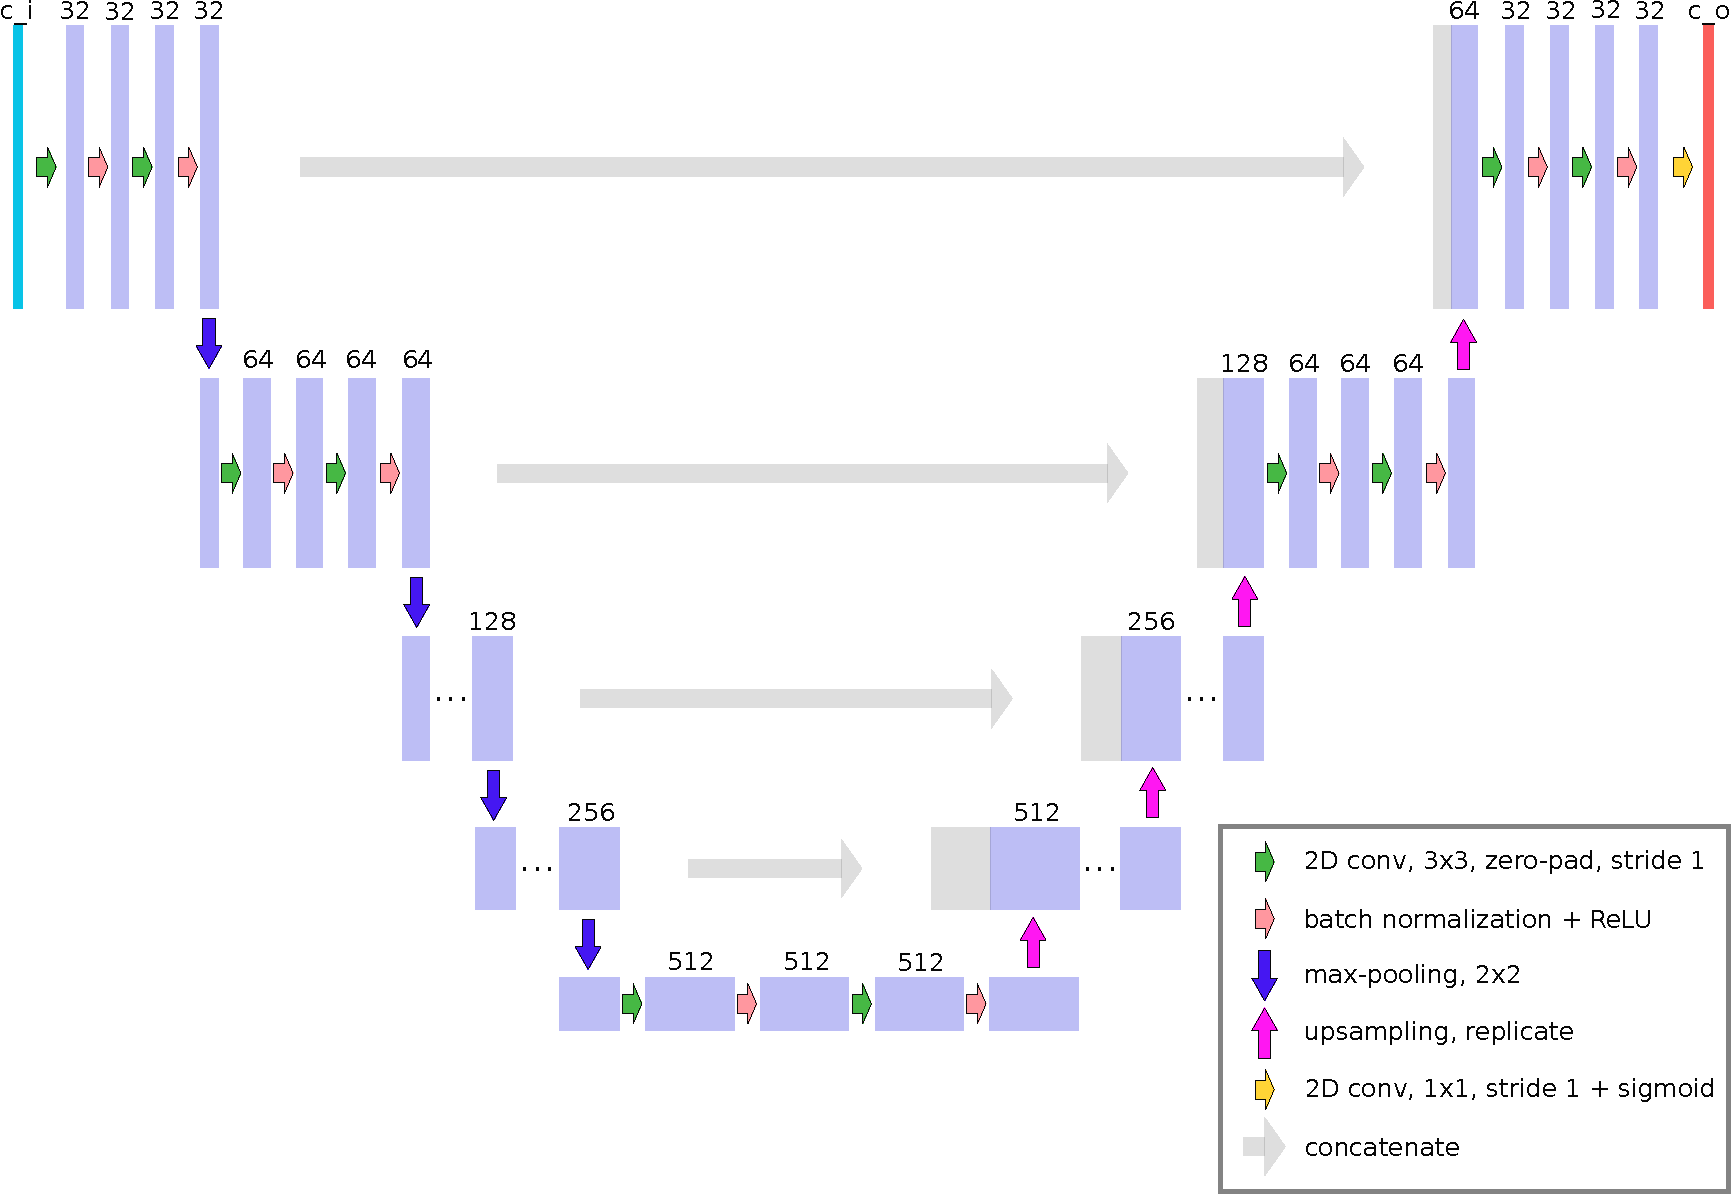
\includegraphics[width=\textwidth]{unet/model5}
  \caption[Modified U-Net architecture]{Illustration of our modified U-Net structure. Other than the original U-Net structure, it has a batch normalization layer after each convolutional layer. Depending on the data color space and loss function, it uses different number of input channels $c\_i$ and output channels $c\_o$.}
  \label{fig:unet_model}
\end{figure}

\subsection{Data Augmentation} \label{ch:data_gen}
Since the datasets we used are rather small in size, we used data augmentation wherever possible to increase the training data size. However, since we have a setting where we train the neural network on the same data we later extract the features from, the model does not need to generalize to non-seen data. Hence, we only use image transforms that are observed within the data. For example, it is very likely that during a slit-lamp recording the user rotates and shifts the camera, resulting in different angles and positions of the optical disc. This confirms to use horizontal and vertical shift, as well as rotation for image transforms. Contrarily, as the size of the object seldom changes, scaling and zooming are not relevant transformations.
The same reasoning applies to other datasets.
To sum up, we resort to rotation, vertical/horizontal translation as well as little shearing. Additionally, we added Gaussian noise for regularization. In our implementation, we used the online data generator provided by the Keras framework \cite{Keras}, which randomly generates new data during training time. Some examples and parameters used are described in chapter \ref{results_data_gen}.

\clearpage
\subsection{Feature Extraction} \label{feat_extract}
Similarly to our baseline methods, U-Net based methods construct a feature matrix $\boldsymbol{X} = [\boldsymbol{x}_1,...,\boldsymbol{x}_S]^T \in \mathbb{R}^{S \times D}$ describing each superpixel. Fig. \ref{fig:feat_extract} illustrates this process on an example of a single image. After training, a forward pass is performed on all image and features are taken as the output (ReLU) of the deepest layer. Those features correspond to a downscaled version of the input image. Hence, it must be upscaled to the original image resolution. Each feature dimension is independently upscaled to the original image size using bicubic interpolation. Since one pixel becomes a region, extrapolation is also needed at border regions, shown by the red circle and square in Fig. \ref{fig:feat_extract}. As we now have a descriptor for each pixel upscaled to the same resolution as the original data, we can take the mean over all descriptors belonging to the individual superpixels with feature dimension $D=512$.
\vspace{10pt}

\begin{figure}[htbp]
  \centering
  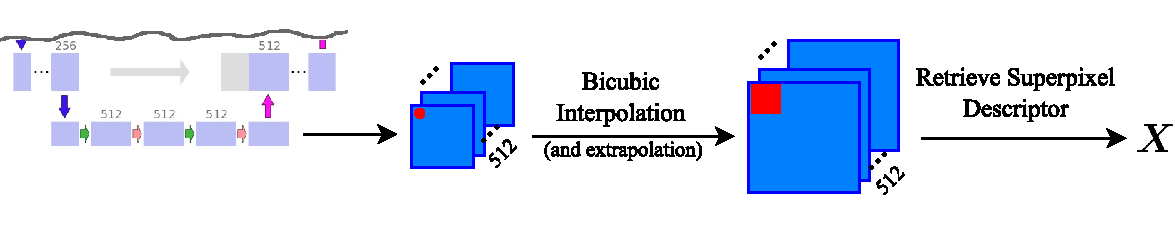
\includegraphics[width=\textwidth]{feat_extract/feature_extraction}
  \caption[Feature extraction model]{Illustration of feature extraction for U-Net based methods. The features are extracted from the deepest level. Those features are then interpolated (and extrapolated) on each dimension individually to obtain the original resolution. Each pixel is described by a feature vector of dimension $D=512$.
    Superpixels are assigned to the mean of all feature vectors that it envelopes.}
  \label{fig:feat_extract}
\end{figure}

\subsection{U-Net Reconstruct}
\begingroup
\setlength\intextsep{0pt}
\begin{wrapfigure}[4]{l}[0pt]{1.4cm}
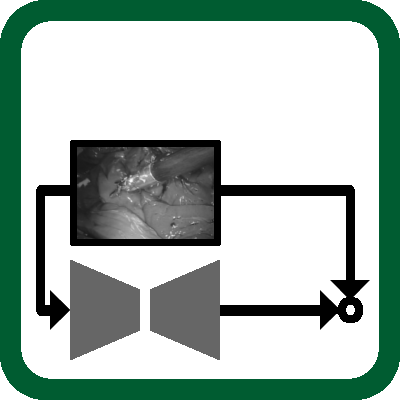
\includegraphics[height=1.5cm]{icons/unet_rec.png}
\end{wrapfigure}

\textit{U-Net Reconstruct} (or \textit{U-Net Rec}) is an unsupervised model. It takes as input the image data and reconstructs the same data. Let $\mathcal{I}$ be the image set and $\boldsymbol{I}_k \in [0,1]^{H \times W \times C}$ an image with height $H$, width $W$ and number of channels $C$. We assume that $\boldsymbol{I}_k$ is already downscaled to have $H$ and $W$ dividable by $16$ (see chapter \ref{model}). Pixels are described by $\boldsymbol{I}_k(i,j,c) \in [0,1]$ with $i$ and $j$ its indices. The reconstructed image, of same dimension as the input, is written $\boldsymbol{\hat{I}}_k$. The network's channel dimensions is taken as $C = c_i = c_o$. We chose to use a mean-squared error (MSE) loss function. For a minibatch of size $B$, the loss is given by:

\endgroup
\vspace{6pt}

\begin{equation}
L_{MSE} = \frac{1}{W H |\mathcal{B}|} \sum_{\boldsymbol{I}_l \in \mathcal{B}} \sum_{i,j,c} \|\boldsymbol{I}_l(i,j,c) - \boldsymbol{\hat{I}}_l(i,j,c)\|^2
\label{eq:mse_loss}
\end{equation}
\vspace{6pt}

Where $\| \cdot \|$ is the $L2$-norm and $\mathcal{B} \subset \mathcal{I}$ is the minibatch.
In later formulations, we will omit the summation on the mini-batch for clarity.

\clearpage
\subsection{U-Net Gaze Reconstruct} \label{unet_gaze_rec}
\begingroup
\setlength\intextsep{0pt}
\begin{wrapfigure}[4]{l}[0pt]{1.4cm}
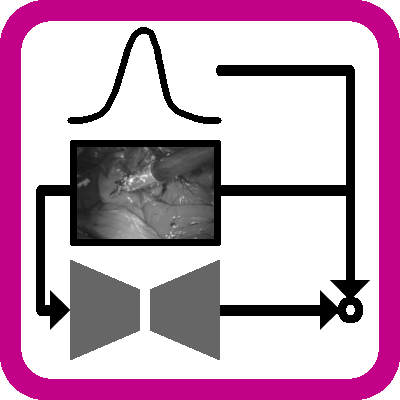
\includegraphics[height=1.5cm]{icons/unet_gaze_rec.png}
\end{wrapfigure}

Similar to \textit{U-Net Rec}, \textit{U-Net Gaze Reconstruct} (or \textit{U-Net Gaze Rec}) trains the network in an autoencoder fashion. This time, we introduce a prior on the gaze location into the loss-function. Let $\boldsymbol{g} = [g_x, g_y]$ be the xy-coordinates of the gaze-point, and  $\boldsymbol{Z} \in [0,1]^{H \times W}$ a probability map. Assuming that the gaze location $\boldsymbol{g}$ is given for an image $\boldsymbol{I}$, we take $\boldsymbol{Z} \sim \mathcal{N}(\boldsymbol{g}, \sigma^2\mathbb{I})$, a 2D-Gaussian distribution with standard deviation $\sigma$ and mean $\boldsymbol{g}$. For images where no gaze locations are available, we take a Uniform distribution. It is formulated in Eq. \ref{eq:gaussian}.

\endgroup

\begin{equation}
\boldsymbol{Z} = 
\begin{cases}
  \mathcal{U}(0,WH),& \textit{if } \boldsymbol{g} \textit{ not available}\\         \mathcal{G}(\boldsymbol{g}, \sigma^2\mathbb{I}),         & \textit{if } \boldsymbol{g} \textit{ available}
\end{cases}
\label{eq:gaussian}
\end{equation}
\hspace{6pt}

$\boldsymbol{Z}_{i,j}$ therefore models the object prior at location $(i,j)$, with $i \in \{\mathbb{Z} \mid 1 \leq i \leq H\}$ and $j \in \{\mathbb{Z} \mid 1 \leq j \leq W\}$ to be the probability of that pixel corresponding to the object of interest. Each pixel's $L2$-norm is then multiplied by $\boldsymbol{Z}_{i,j}$. The loss function is therefore given by:

\begin{equation}
L_{MSE\_Gaze} = \frac{1}{W H} \sum_{i,j} \frac{\boldsymbol{Z}_{i,j}}{\max{\{\boldsymbol{Z}\}}} \|\boldsymbol{I}_{i,j} - \boldsymbol{\hat{I}}_{i,j}\|^2
\label{eq:mse_gaze_loss}
\end{equation}
\hspace{6pt}

Where we normalize by $\max{\{\boldsymbol{Z}\}}$ for later comparison with the loss of \textit{U-Net Rec}. This model, therefore, penalizes errors situated near the gaze-point. In most image modalities, the object of interest is only a small portion of the image and distinctive. Contrarily, the background is rather regular or even fully black, as it usually is for CT and MRI scans. Hence, we can reason that penalizing the loss in regions of interest equalizes the weights given to background and object of interest in terms of area occupied by the foreground, resp. background.

\subsection{U-Net Gaze Probability Map} \label{unet_gaze_prob_map}
\begingroup
\setlength\intextsep{0pt}
\begin{wrapfigure}[4]{l}[0pt]{1.4cm}
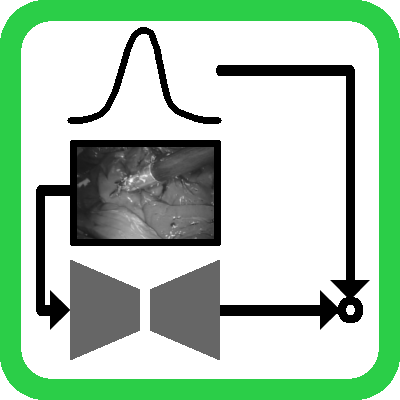
\includegraphics[height=1.5cm]{icons/unet_gaze_prob.png}
\end{wrapfigure}

\textit{U-Net Gaze Probability Map} (or \textit{U-Net Gaze Prob}) predicts a probability map of the gaze location given the image. We use the same formulation for the probability map $\boldsymbol{Z}$ as for \textit{U-Net Gaze Rec} method in chapter \ref{unet_gaze_rec}. The model's output is now given by $\boldsymbol{\hat{Z}} \in [0,1]^{H \times W}$. In the work of Kurmann at al. \cite{kurmann17}, they used a similar setting and showed that a binary-cross-entropy loss (BCE-loss) performs well. This gave rise to use BCE-loss, formulated in Eq. \ref{eq:mse_gaze_prob_loss} on an example of one image. The network's channel dimensions are $c\_i=C$ and $c\_o=1$.

\endgroup
\begin{equation}
L_{BCE} = \frac{1}{W H} \sum_{i,j} \boldsymbol{Z}_{i,j} \log{\boldsymbol{\hat{Z}}_{i,j}} + (1-\boldsymbol{Z}_{i,j}) \log{(1-\boldsymbol{\hat{Z}}_{i,j})}
\label{eq:mse_gaze_prob_loss}
\end{equation}
\hspace{6pt}

\clearpage
\subsection{U-Net Gaze Probability Map Freezed}
\begingroup
\setlength\intextsep{0pt}
\begin{wrapfigure}[4]{l}[0pt]{1.4cm}
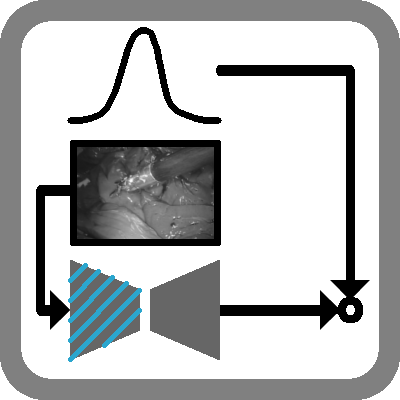
\includegraphics[height=1.5cm]{icons/unet_gaze_prob_freeze.png}
\end{wrapfigure}

\textit{U-Net Gaze Probability Map Freezed} (or \textit{U-Net Gaze Prob Freeze}) combines the benefits of \textit{U-Net Rec} and \textit{U-Net Gaze Prob}. The model is first trained as an autoencoder similarly to \textit{U-Net Rec}. Encoder weights are then frozen (or fixed), and the model is re-trained in a similar fashion to \textit{U-Net Gaze Prob}. Fig. \ref{fig:model_freeze} shows the network's portion where weights are frozen. We can see that the only layers that affect the feature extraction are the ones located at the lowest level. This method is aimed at leveraging benefits of an autoencoder setting in \textit{U-Net Rec} and benefits by using the gaze prior as in \textit{U-Net Gaze Prob}.

\endgroup

\begin{figure}[htbp]
  \centering
  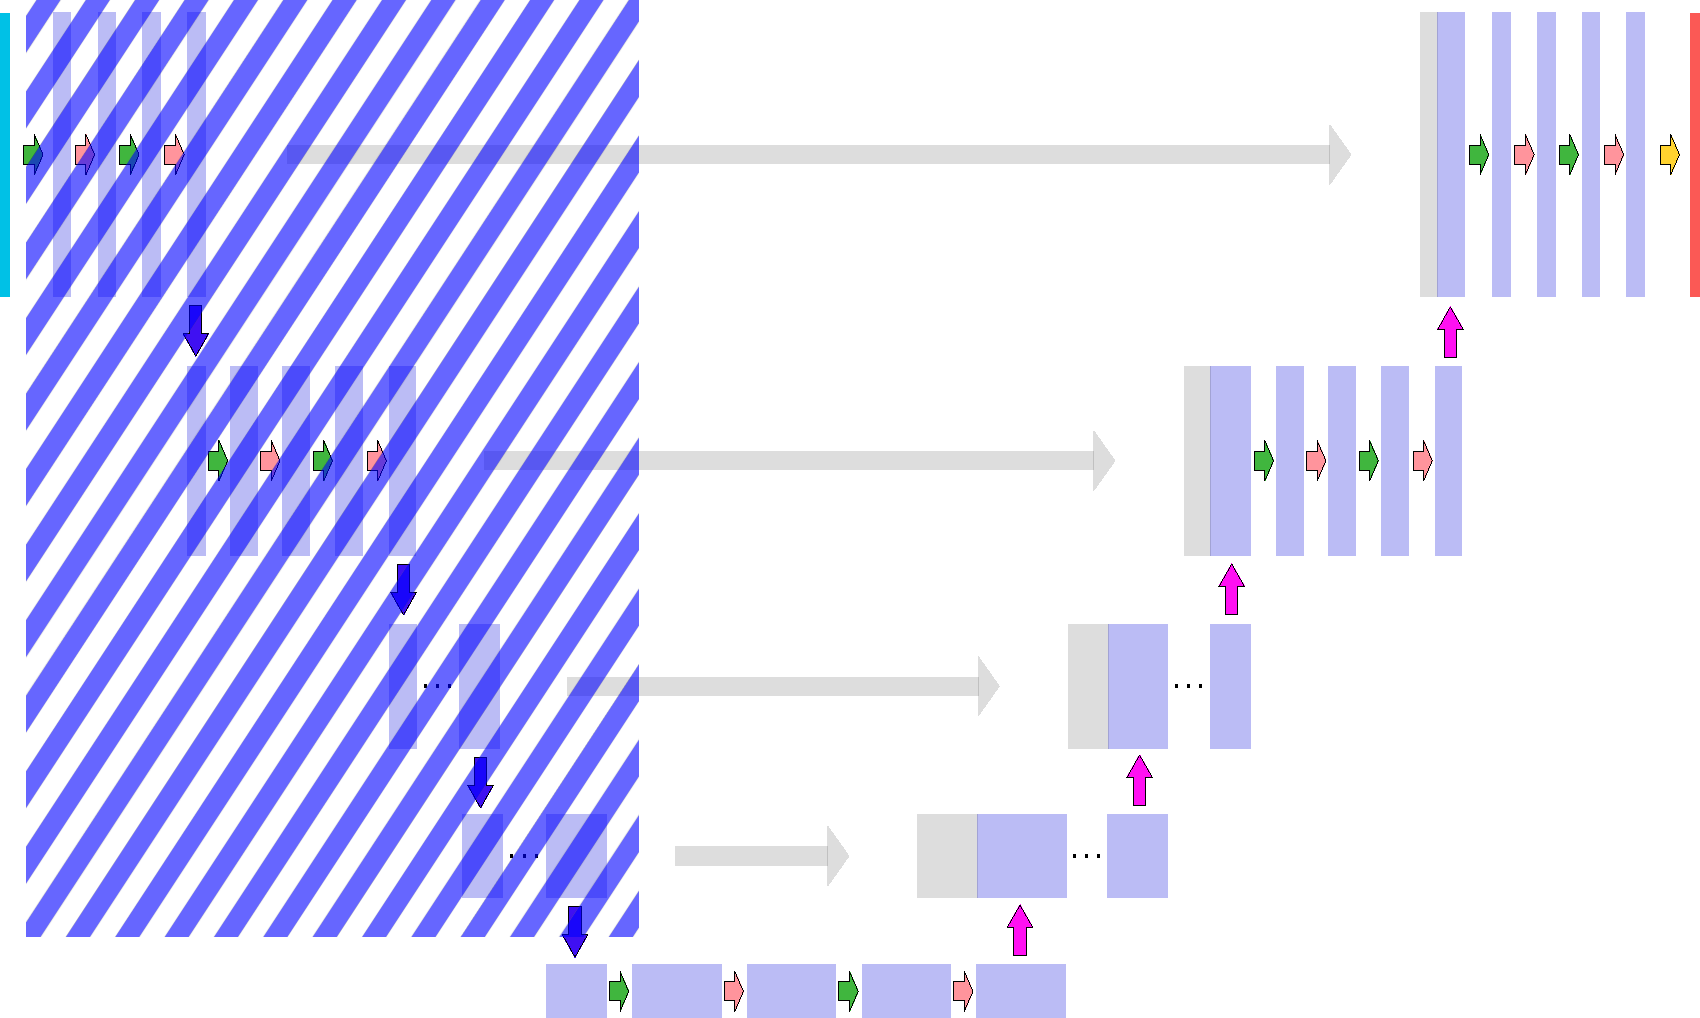
\includegraphics[width=5.0cm]{unet/model5_coarse}
  \caption[Modified U-Net with freezed encoder part]{Illustration of frozen layers in \textit{U-Net Gaze Prob Freeze} method. All encoder part except the lowest level is frozen.}
  \label{fig:model_freeze}
\end{figure}

\subsection{U-Net Gaze Probability Map Concatenate} \label{unet_gaze_prob_concat}
\begingroup
\setlength\intextsep{0pt}
\begin{wrapfigure}[4]{l}[0pt]{1.4cm}
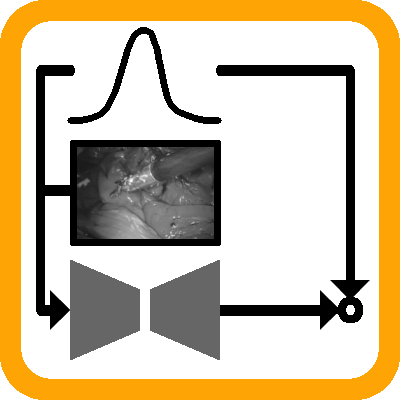
\includegraphics[height=1.5cm]{icons/unet_gaze_prob_concat.png}
\end{wrapfigure}

This model is based on the assumption that objects of interest in our context have relatively slow motion. In other words, the current gaze location is correlated to the previous gaze location(s). We therefore aim at predicting the object's current location. \textit{U-Net Gaze Probability Map Concatenate} (or \textit{U-Net Gaze Prob Concat}) incorporates the data's temporal correlation.

\endgroup

Similar to \cite{lea16}, who investigated the problem of fine-grained action segmentation, we increased the model's number of input channel by a motion image. However, we followed a more straightforward approach by adding as motion information the previous probability map $\boldsymbol{Z}^{(t-1)}$.

Fig. \ref{fig:unet_gaze_concat} illustrates the overall structure on one image $\boldsymbol{I}$. The gaze probability map at time $t-1$, shown as $\boldsymbol{Z}^{(t-1)}$, is concatenated to $\boldsymbol{I}^{(t)}$. These taken as inputs are then used to predict the gaze location at time $t$, defined by $\boldsymbol{\hat{Z}}^{(t)}$. Similar to \textit{U-Net Gaze Prob}, we used BCE-loss.

\begin{figure}[htbp]
  \centering
  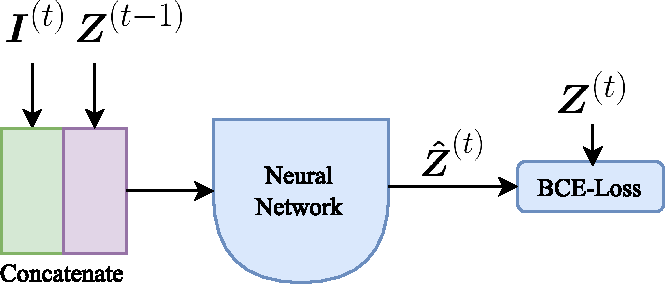
\includegraphics[width=7cm]{unet/unet_gaze_concat}
  \caption[Structure of U-Net Gaze Prob Concat]{Structure of U-Net based method \textit{U-Net Gaze Prob Concat}. The previous gaze probability map $\boldsymbol{Z}^{(t-1)}$ is concatenated to the current image data $\boldsymbol{I}^{(t)}$. Out of those informations, the Neural Network predicts the current gaze location $\boldsymbol{Z}^{(t)}$.}
  \label{fig:unet_gaze_concat}
\end{figure}

Since we augmented the inputs by an additional channel, the model's channel dimension become $c\_i=C+1$ and $c\_o=1$. Note that in this configuration, the ordering of input frame is substantial. Thus, it made it difficult to apply data augmentation procedure. Due to time limitations, we did not use data augmentation.

\subsection{U-Net Gaze Probability Map LSTM} \label{ch:unet_gaze_prob_lstm}
\begingroup
\setlength\intextsep{0pt}
\begin{wrapfigure}[4]{l}[0pt]{1.4cm}
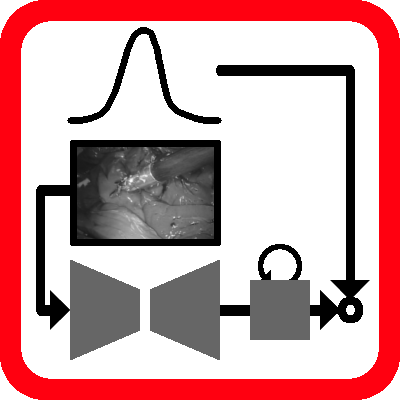
\includegraphics[height=1.5cm]{icons/unet_gaze_prob_lstm}
\end{wrapfigure}

\textit{U-Net Gaze Probability Map LSTM} (or \textit{U-Net Gaze Prob LSTM}) also incorporates the temporal correlation of the object. It uses three models from \textit{U-Net Gaze Prob} with shared weights to predict three consecutive gaze probability maps. Those predicted probability maps are again fed to a recurrent unit, more precisely a convolutional long-short-term-memory (CLSTM) \cite{shi15}, to predict the next gaze location. Fig. \ref{fig:unet_gaze_lstm} illustrates this structure. The CLSTM uses filters of size $3 \times 3$ and no return sequence.

\endgroup

\begin{figure}[htbp]
  \centering
  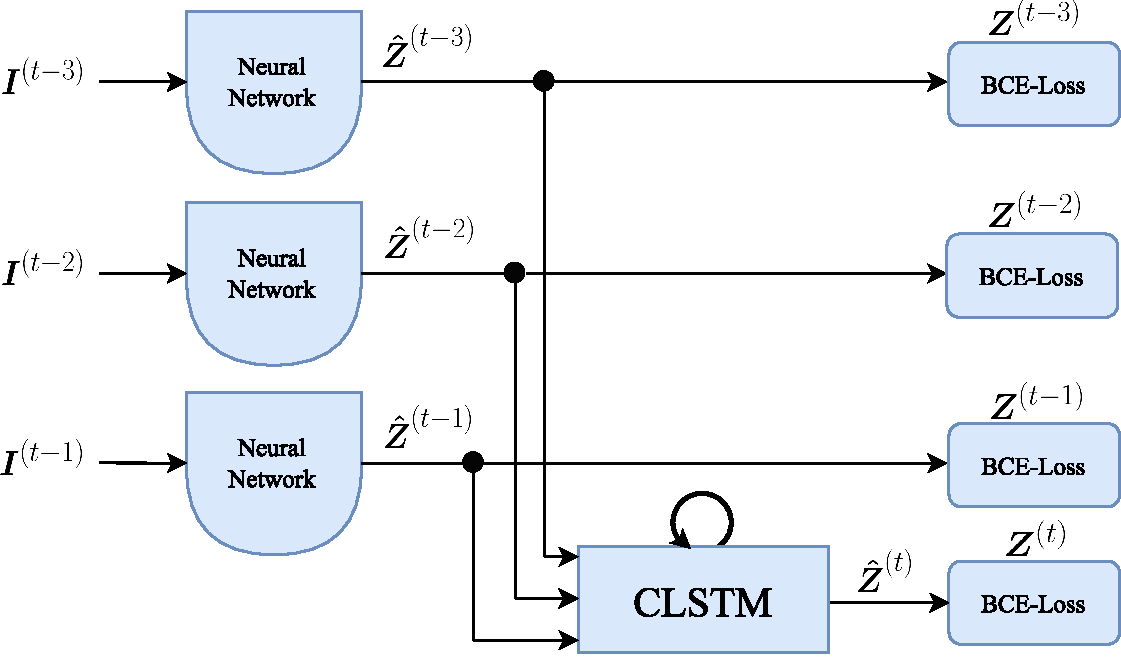
\includegraphics[width=10cm]{unet/unet_gaze_lstm}
  \caption[Structure of U-Net Gaze Prob Map LSTM]{Structure of U-Net based method \textit{U-Net Gaze Prob LSTM}. A sequence of three images is fed to three identical U-Net models as in \textit{U-Net Gaze Prob} with shared weights. The predicted gaze probability maps $\boldsymbol{\hat{Z}}$ are fed to a CLSTM, predicting the next gaze. The overall loss is a mix of all four BCE-losses.}
  \label{fig:unet_gaze_lstm}
\end{figure}

The overall loss $L_{BCE\_LSTM}$ for one image sequence of three images is shown in Eq. \ref{eq:bce_lstm}. $L_{BCE}(A,B)$ defines the binary cross entropy, formulated in Eq. \ref{eq:mse_gaze_prob_loss}, between $A$ and $B$. Parameter $\alpha$ is used to adjust the weight of the CLSTM prediction. We used some jittering to represent the data, i.e. one sample is given by the sequence $[\boldsymbol{I}^{(t=0)}, \boldsymbol{I}^{(t=1)}, \boldsymbol{I}^{(t=2)}]$, and $[\boldsymbol{I}^{(t=1)}, \boldsymbol{I}^{(t=2)}, \boldsymbol{I}^{(t=3)}]$ represents another sample. Likewise to the method \textit{U-Net Gaze Prob Concat}, we did not synthesize more data by using any sort of data augmentation.

\begin{equation}
L_{BCE\_LSTM} = \alpha \Big[\sum_{d=1}^3 L_{BCE}(\boldsymbol{\hat{Z}}^{(t-d)}, \boldsymbol{Z}^{(t-d)})\Big] + (\alpha - 1) L_{BCE}(\boldsymbol{\hat{Z}}^{(t)}, \boldsymbol{Z}^{(t)})
\label{eq:bce_lstm}
\end{equation}
\hspace{6pt}

\clearpage
\subsection{U-Net Based Methods Overview}
Tab. \ref{tab:summary_unet_methods} summarizes the U-Net based methods. To recap, $C$ is the number of image channels ($1$ for grayscale and $3$ for colored) and $c\_i$, $c\_o$ the number of the networks input and output channels, respectively.

\begin{table}[!htbp]
   \centering
   \caption[U-Net based method overview]{Overview of U-Net based methods with $C$ being the number of channels in the images and $c\_i$, $c\_o$ the network's input and output channel dimension, respectively.}
   \begin{tabular}{l|m{1.3cm}|c|c|c|c}
      \toprule
      \textbf{Method} & \textbf{Symbol} & \textbf{Inputs} & \textbf{Labels} & \textbf{c\_i} & \textbf{c\_o} \\
      \midrule
      U-Net Rec & 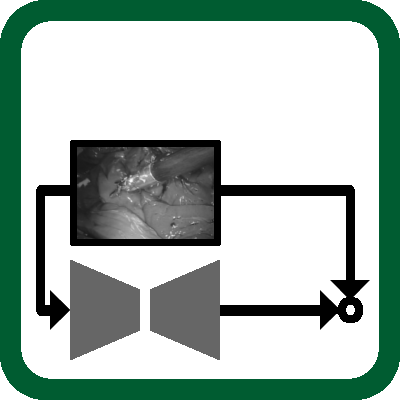
\includegraphics[width=1cm]{icons/unet_rec.png} & Image & Image & $C$ & $C$ \\
      \midrule
      U-Net Gaze Rec & 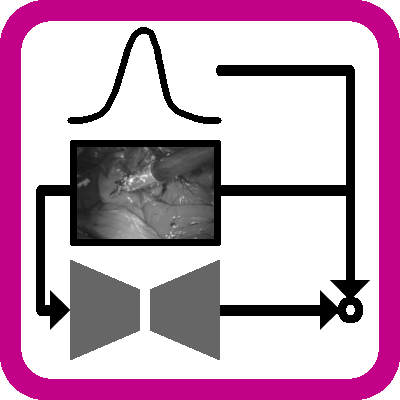
\includegraphics[width=1cm]{icons/unet_gaze_rec.png} & Image & Image \& Gaze & $C$ & $C$ \\
      \midrule
      U-Net Gaze Prob & 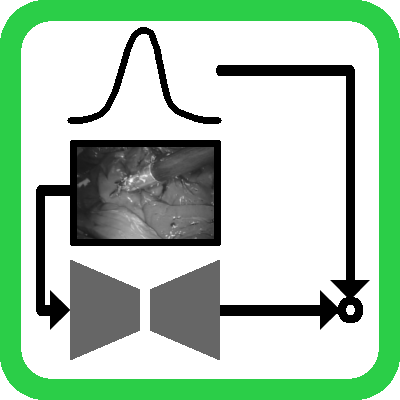
\includegraphics[width=1cm]{icons/unet_gaze_prob.png} & Image & Gaze & $C$ & $1$ \\
      \midrule
      U-Net Gaze Prob Freeze & 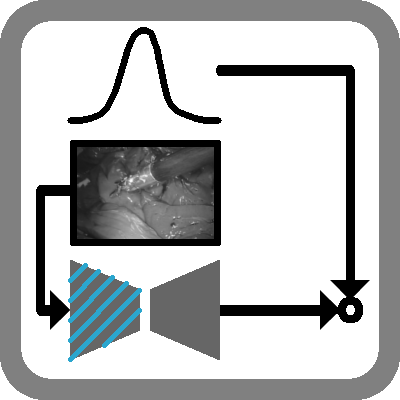
\includegraphics[width=1cm]{icons/unet_gaze_prob_freeze.png} & Image & Gaze & $C$ & $1$ \\
      \midrule
      U-Net Gaze Prob Concat & 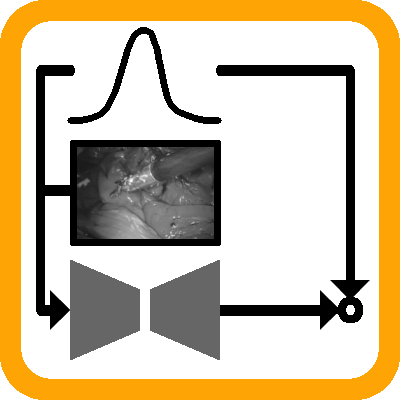
\includegraphics[width=1cm]{icons/unet_gaze_prob_concat.png} & Image \& Gaze & Gaze & $C+1$ & $1$ \\
       \midrule
      U-Net Gaze Prob LSTM & 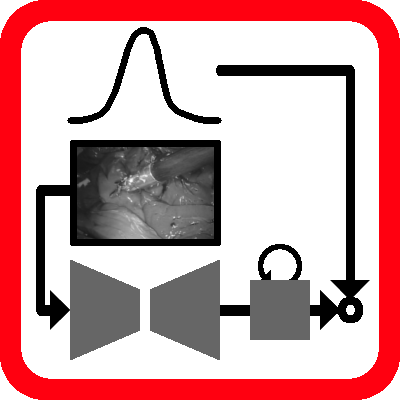
\includegraphics[width=1cm]{icons/unet_gaze_prob_lstm.png} & Image Sequence & Gaze & $3 \times C$ & $3 \times 1$ \\
      \bottomrule
   \end{tabular}
   \label{tab:summary_unet_methods}
\end{table}

%\myworries{
%\begin{itemize}
%  \item Training time (one paragraph)
%\end{itemize}}

\section{Evaluation Method}
We used a random forest classifier to compare the performance between the different feature learning methods. How this classifier is applied and configured, is described in a first section. Later, we describe the measures, which allow us to compare the performance among one another method.

\subsection{Random Forest} \label{random_forest}
To compare performance between the elaborated methods, we set up a Random Forest classifier, as shown in Fig. \ref{fig:random_forest}.
It takes as input a feature matrix $\boldsymbol{X} \in \mathbb{R}^{S \times D}$ and labels $\boldsymbol{y} \in \{0,1\}^{S}$ of one image data sequence.
As described in chapter \ref{framework}, $S$ is the number of superpixels in one sequence and $D$ the feature dimension.
Firstly, labels $\boldsymbol{y}$ and feature matrix $\boldsymbol{X}$ are both similarly shuffled.
Then, it uses k-fold cross-validation on $5$ folds to train the classifier and validate.
This ensures that each data point belonged one time to the validation set $\boldsymbol{X}_V$, resp. $\boldsymbol{y}_V$ and $4$ times to the training set $\boldsymbol{X}_T$, resp. $\boldsymbol{y}_T$. All $5$ validation sets are individually evaluated, a precision-recall curve drawn as well as a \textit{max F1-Score} calculated. The final performance measure is the average over all $5$ folds. Since we usually have very few positive labels, we paid attention that each validation set contains more or less the same number of positive labels.

\begin{figure}[htbp]
  \centering
  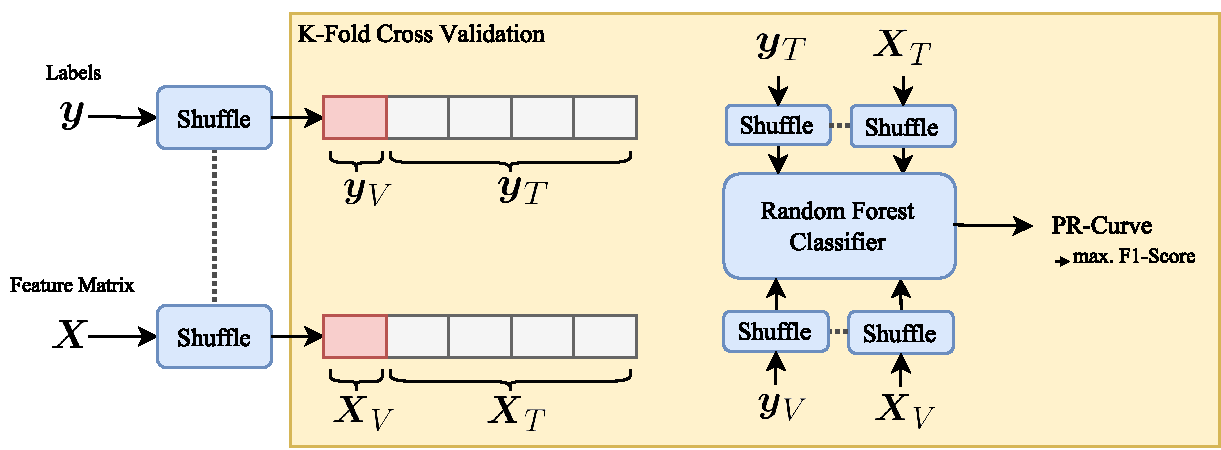
\includegraphics[width=14cm]{random_forest/random_forest}
  \caption[Illustration of Random Forest classifier]{Set-up of Random Forest classifier for evaluating performance of feature learning methods. It learns a Random Forest classifier on superpixel labels $\boldsymbol{y}$ and feature matrix $\boldsymbol{X}$ of one image data sequence. Since the datasets are rather small in size and have few positive labels, validation is done by a k-fold cross-validation.}
  \label{fig:random_forest}
\end{figure}

In our Random Forest classifier, all nodes are expanded until the leaves are pure.
There is a big discussion whether pruning trees help random forest for better performance.
Segal \cite{segal04} revealed that gains can be obtained by regulating tree size.
However, \cite[pg. 596]{hastie09} notices that those performance gains are rather small. We stuck to Hastie et al.'s conclusion and took advantage of one less tuning parameter.

We built the forest out of $150$ trees and used $m=\sqrt{p}$, where $m$ is the number of selected predictor variables and $p$ the number of all predictor variables. For implementation, we used the sklearn package \cite{scikit-learn}.

\subsection{Precision-Recall Curve}
Precision Recall curves (PR-curves) are a performance measure commonly used for binary decision problems in machine learning.
We used PR-curves to evaluate the results of our Random Forest classifier, and thus, PR-curves present the performance of a feature learning method on a dataset.
We also tried using Receiver Operation Characteristics (ROC) as a measure, but it turned out that PR-curves are a more useful measure for our data.
This might be due to the nature of our data.
Since we usually have much more negative than positive labels, our data becomes skewed.
PR-Curves are more informative than ROC for skewed data, as pointed out by \cite{davis06}. They also stated that a curve dominates in ROC space if and only if it dominates in PR space.

As described in chapter \ref{random_forest}, the final performance measure of an algorithm is the average over all five cross validation folds. By this means, the variance is minimized.

\clearpage
\subsection{Max F1-Score} \label{ch:scores}
F1-Score is a measure that considers both, recall and precision. It's best value is reached at $1$ and worst at $0$. The formula is given by Eq. \ref{eq:f1_score}.

\begin{equation}
\textrm{F1-Score} = 2 \cdot \frac{\textrm{Precision} \cdot \textrm{Recall}}{\textrm{Precision} + \textrm{Recall}}
\label{eq:f1_score}
\end{equation}
\hspace{6pt}

\textit{Max F1-Score} is defined as the relationship between precision and recall that reaches the maximum score. It can be seen as calculating for all points in a PR-curve, their according F1-Scores and taking the maximum. An example is given in Fig. \ref{fig:f1_score}, where the left diagram shows a PR-curve and the right diagram the F1-Score given the Recall values. The maximum value is shown in green.

\begin{figure}[ht]
  \centering
  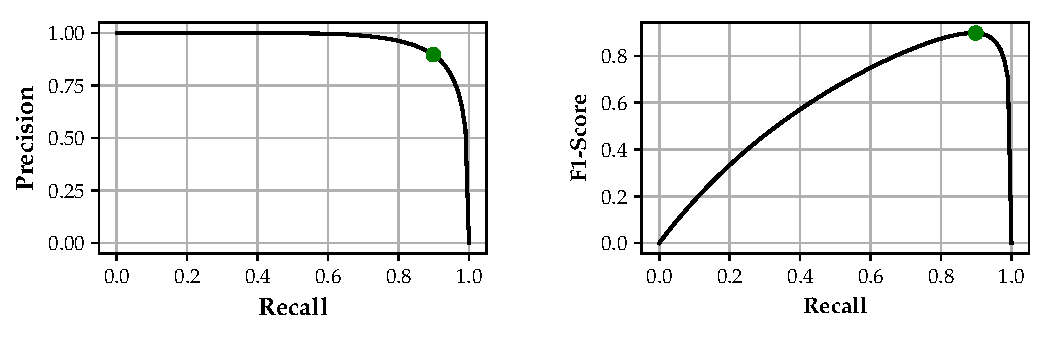
\includegraphics[width=11cm]{f1_score/f1_score}
  \caption[Illustration of max F1-Score]{Illustration of \textit{max F1-Score}. The left diagram shows an example of a \textit{Precision Recall curve}. The diagram on the right shows the F1-Score given the \textit{Recall} values. Maximum score is marked by a green point, the \textit{max F1-Score}.}
  \label{fig:f1_score}
\end{figure}

%%% Local Variables:
%%% mode: latex
%%% TeX-master: "../../main"
%%% End:

% %%%%%%%%%%%%%%%%%%%%%%%%%%%%%%%%%%%%%%%%%%%%%%%%%%%%%%%%%%%%%%%%%%%%%%%%
% Related Work and Background
%%%%%%%%%%%%%%%%%%%%%%%%%%%%%%%%%%%%%%%%%%%%%%%%%%%%%%%%%%%%%%%%%%%%%%%%
%
% Author:   Jan Grossrieder
%           Ophthalmic Technology Laboratory
%           ARTORG Center Bern
%           jan.grossrieder@students.unibe.ch
%
% Date:     07/18/2017
%
%%%%%%%%%%%%%%%%%%%%%%%%%%%%%%%%%%%%%%%%%%%%%%%%%%%%%%%%%%%%%%%%%%%%%%%%

\chapter{Results}
This chapter starts by giving visual results of our superpixel segmentation. We then elaborate on the experimental setup. The results from training and evaluation procedures are described. Details on method-specific parameters and configuration are also given.

\section{Superpixel Segmentation}
Fig. \ref{fig:sp_example} shows examples of the superpixel segmentation. The yellow line shows the ground truth contour of the object of interest and the red line the contour made by the superpixels. We notice that in the surgical video recording the segmentation often misses the contour of the tweezer. In the CT recording of the inner ear, a small region is not captured by the superpixel segmentation. 

\begin{figure}[htbp]
  \centering
  \subfloat[Surgical Video]
  {
    \label{fig:subfig:sp_example_01}
    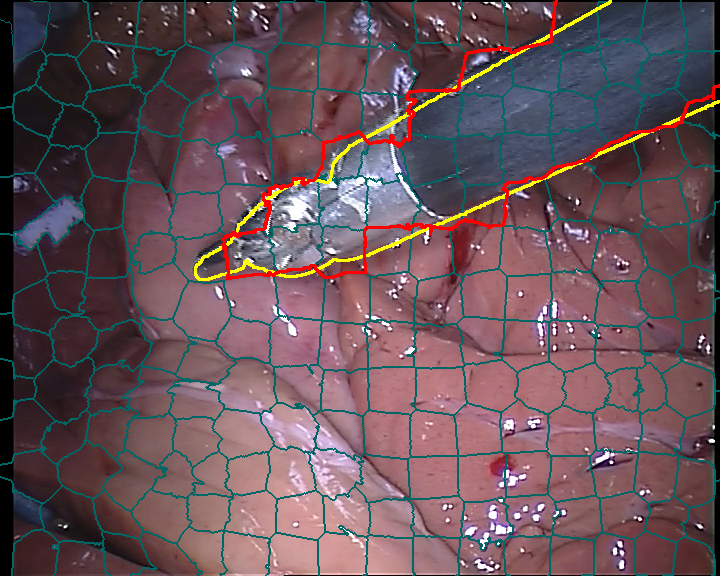
\includegraphics[width=4.1cm]{superpixel_results/ds_01}
  }
  \hspace{2cm}
  \subfloat[Slit-Lamp Retina A]
  {
    \label{fig:subfig:sp_example_12}
    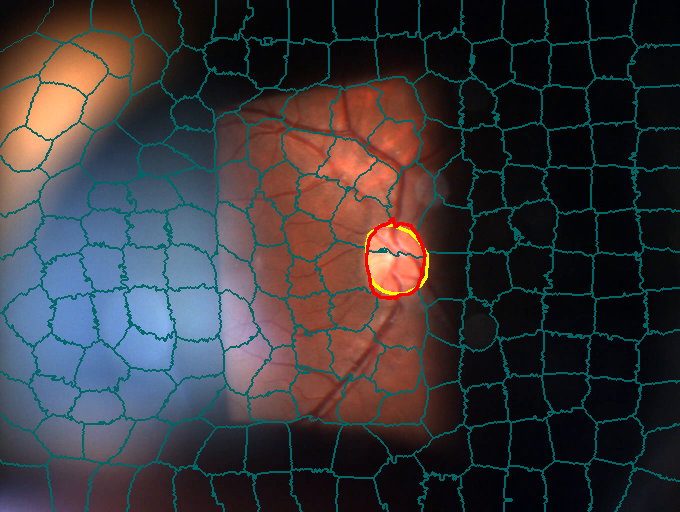
\includegraphics[width=4.1cm]{superpixel_results/ds_12}
  }
  \\
  \subfloat[MRI Brain A]
  {
    \label{fig:subfig:sp_example_09}
    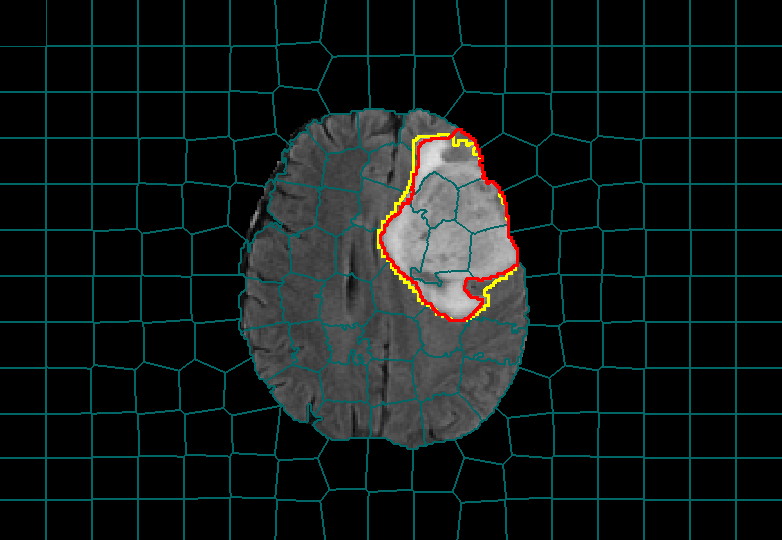
\includegraphics[width=4.1cm]{superpixel_results/ds_09}
  }
  \hspace{2cm}
  \subfloat[CT Inner Ear A]
  {
    \label{fig:subfig:sp_example_11}
    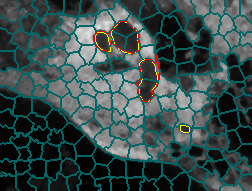
\includegraphics[width=4.1cm]{superpixel_results/ds_11}
  }
  \caption[Superpixel segmentation example]{Illustration of errors in superpixel segmentation. The object of interest is marked in yellow. Superpixels are shown in dark green and all superpixels which are assigned to positive labels are contoured in red. In (a) the segmentation misses the object contour. In (b) and (c), the segmentation follows the contours more accurately. In (d), a small region is missed.}
  \label{fig:sp_example}
\end{figure}

We also performed experiments with the non-adaptive superpixel segmentation method SLIC.
This method showed to follow better the contours with the cost of having highly irregular shaped segments (as also shown by \cite{csillik16}).
We concluded that for our task, regularly shaped segments are more important and therefore used the ASLIC method.

\section{Neural Network Training}
In this section, we first describe the training configurations followed by the parameterization of the data augmentation. We then analyze the training loss (learning curves) on few examples.
Visual examples of activation maps are given to illustrate what kind of filters the network is learning.

\subsection{Training Configurations} \label{ch:training_conf}
All of our U-Net based models are trained using an Adam optimizer \cite{kingma15} (learning rate $= 0.0001$, $\beta_1 = 0.9$, $\beta_2 = 0.999$, $\epsilon = 10^{-8}$, no decay), and Glorot \cite{glorot10} to initialize the weights.
The stopping criterion for training is reached after $20$ epochs. We will argue about this value in chapter \ref{ch:perf_vs_training}.

The maximum size of the mini-batch depends on the GPU memory, the model architecture, and since the latter has different input sizes, also the resolution of the input data. We trained our models on a \textit{GeForce GTX 1080 Ti}, with 11GB memory. The model architectures are all similar in size except for the \textit{U-Net Gaze Prob LSTM}, which contains another recurrent part. The datasets also have similar resolution except for the \textit{CT Inner Ear A + B}. Tab. \ref{tab:batch_size} shows the used mini-batch size.
\vspace{30pt}

\begin{table}[htbp]
   \centering
   \caption[Mini-batch size]{Mini-batch size used for training U-Net based methods. All methods are trained on a \textit{GeForce GTX 1080 Ti} GPU. Since the CT datasets are smaller in resolution, we could take larger mini-batches. The \textit{U-Net Gaze Prob LSTM} has a larger model and uses, therefore, smaller mini-batches.}
   \begin{tabular}{|c||c|c|}
      \hline
      \diagbox{Dataset}{Method} & \textbf{U-Net Gaze Prob LSTM} & \textbf{All others} \\
      \hline
      \hline
      \Gape[2pt][2pt]{\textbf{\makecell[c]{CT Inner Ear\\ A + B}}} & 4 & 16 \\
      \hline
      \Gape[11pt][11pt]{\textbf{All others}} & 1 & 4 \\
      \hline
   \end{tabular}
   \label{tab:batch_size}
\end{table}

\clearpage
\subsection{Data Augmentation} \label{results_data_gen}
Since we were limited in data size, we had to use an augmentation method (chapter \ref{ch:data_gen}). A data generator samples from the raw image sequence, randomly chooses a value within the given transform range, and applies this transform to the sampled image. Additionally, random Gaussian noise is added to all channels of the image. The amount of Gaussian noise to be added is defined by a standard deviation $\sigma$, which is relative to the $8$bit image depth ($0$ - $255$). Another parameter describes how many samples are generated for each epoch.

The data generator's parameters are defined in Tab. \ref{tab:data_gen_param}. In Fig. \ref{fig:data_gen}, we show examples obtained from a frame out of the dataset \textit{Slit-Lamp Retina A}.
\vspace{20pt}

\begin{table}[!htbp]
   \centering
   \caption[Data generator parameters]{Parameters of data generator. Rotation, translation, and shearing are used as transformation. Gaussian noise is also added to augment data variance. It is defined by the standard deviation $\sigma$, which is relative to the range in bit depth $0-255$. $2'000$ images are randomly sampled for each epoch.}
   \begin{tabular}{l|c}
      \toprule
      \textbf{Parameter} & \textbf{Value} \\
      \midrule
      Rotation range & $\pm11.25$° \\
      Horizontal translation range & $20\%$ of image width \\
      Vertical translation range & $20\%$ of image height \\
      Shearing range & $\pm22.5$° \\
      \midrule
      Gaussian noise $\sigma$ & $13$ \\
      \midrule
      Number of samples per epoch & $2'000$ \\
      \bottomrule
   \end{tabular}
   \label{tab:data_gen_param}
\end{table}
\vspace{30pt}

\begin{figure}[!htbp]
  \centering
  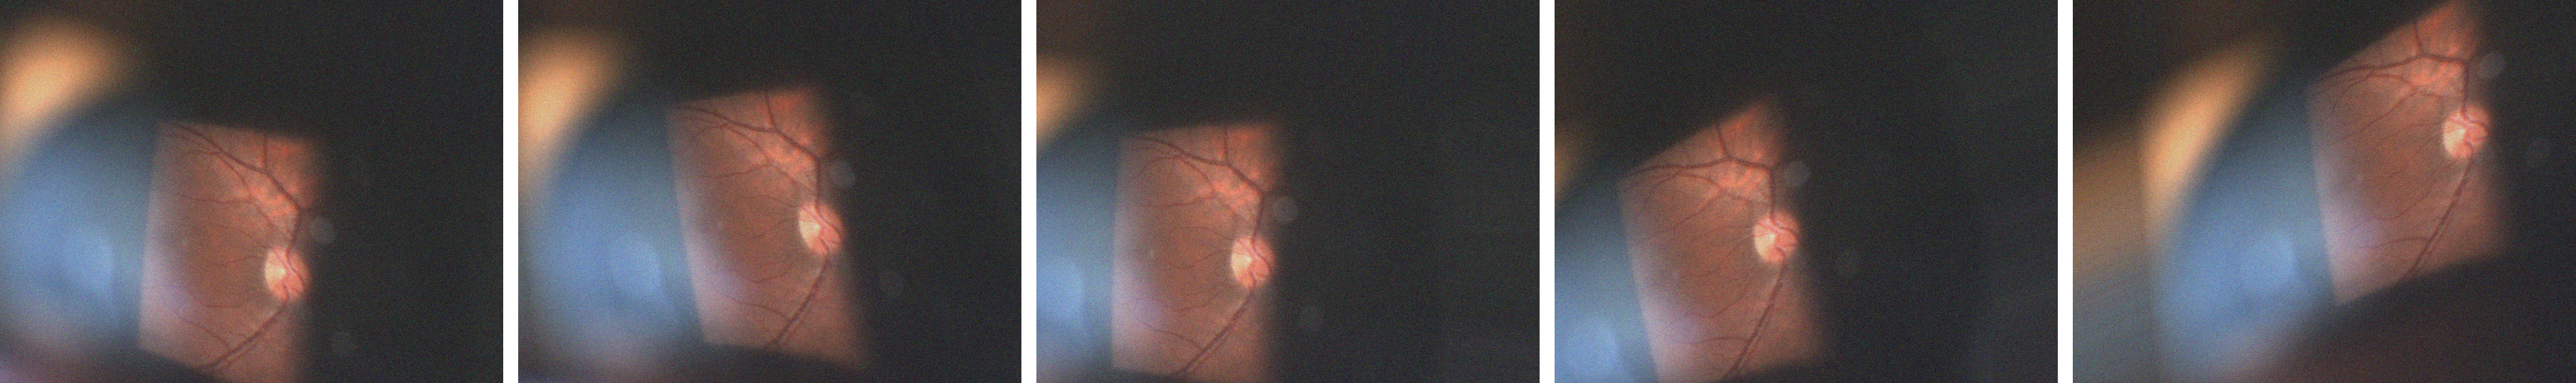
\includegraphics[width=\textwidth]{unet/data_gen}
  \caption[Examples of data generator]{Examples of data generator on an image of dataset \textit{Slit-Lamp Retina A}. We used rotation, translation, shearing and added Gaussian noise to each of the channels. The values are shown in Tab. \ref{tab:data_gen_param}.}
  \label{fig:data_gen}
\end{figure}

\clearpage
\subsection{Learning Curve} \label{ch:learning_curve}
In our setting, we train the CNN model on the dataset we later extract the features from. Thus, there is no need to split the dataset into training and validation. The performance would even become worse since the model would be trained on fewer data. For our datasets, where all frames within the set are very similar to each other, we do not expect to find any signs of overfitting given the learning curve.

However, since we will later describe an experiment that shows the feature performance versus the training time of the model (chapter \ref{ch:perf_vs_training}), we still investigate the training curve. To do so, we took the \textit{CT Inner Ear A} dataset and randomly split it into $80\%$ training set and $20\%$ validation set. Subsequently, we trained two models, namely a \textit{U-Net Rec} with MSE-loss and a \textit{U-Net Gaze Prob} with BCE-loss, for $500$ epochs. After each trained epoch, we calculated training and validation loss. Fig. \ref{fig:learn_curve} shows the training and validation loss for the given models. As we expected, there is no sign of overfitting. We also performed this experiment on other datasets and they all showed similar behaviour.
\vspace{20pt}

\begin{figure}[!htbp]
  \centering
  \subfloat[Learning curve of model \textit{U-Net Rec} on dataset \textit{CT Inner Ear A}]
  {
    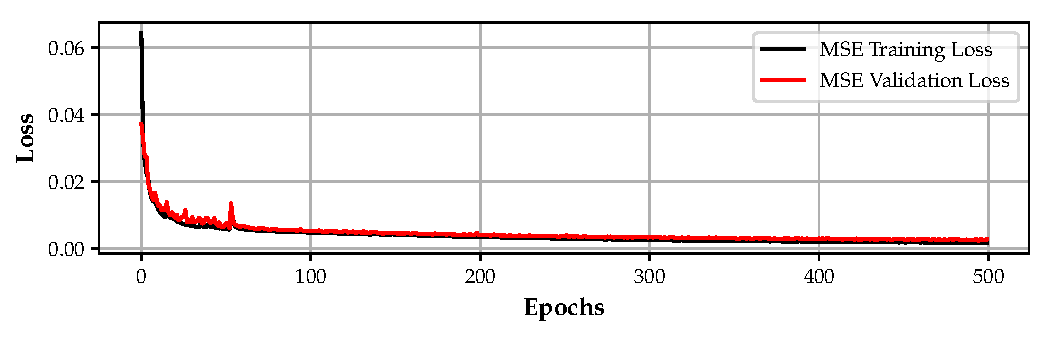
\includegraphics[width=11cm]{learning_curve/learning_curve_ds11_rec}
  }
  \\
  \subfloat[Learning curve of model \textit{U-Net Gaze Prob} on dataset \textit{CT Inner Ear A}]
  {
    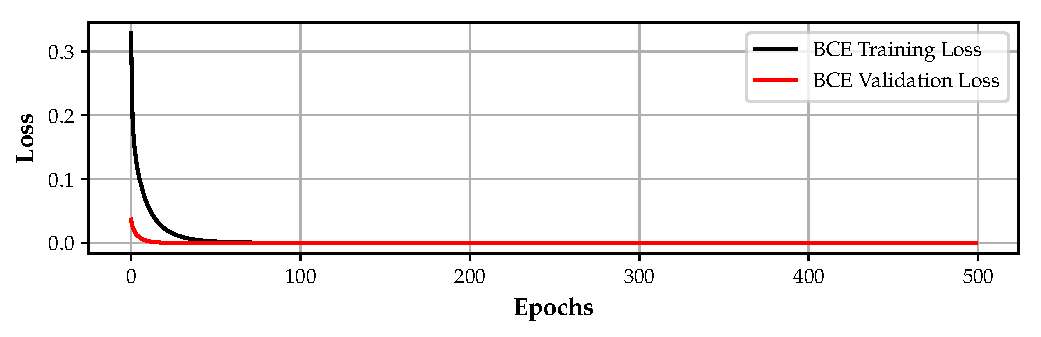
\includegraphics[width=11cm]{learning_curve/learning_curve_ds11_prob}
  }
  \caption[Model learning curves]{Learning curves of training (a) \textit{U-Net Rec} and (b) \textit{U-Net Gaze Prob} model on dataset \textit{CT Inner Ear A}. We split the dataset into $80\%$ training and $20\%$ test and calculated the given loss after each trained epoch. As expected, there are no signs of overfitting.}
  \label{fig:learn_curve}  
\end{figure}
\vspace{20pt}

The time per epoch largely depends on the input size of the model. If using the data generator with the above-mentioned settings and train the model on the stated hardware, it takes at most $4.5$ minutes per epoch (dataset \textit{Surgical Video Sequence}) and at least $35$ seconds per epoch (dataset \textit{CT Inner Ear A}).

\clearpage
\subsection{Activation Maps} \label{ch:act_maps}
To visualize the effect of filters (kernels) in a CNN, one often visualizes their activation during a forward pass.
The examples that follow correspond to the layer where our features are extracted, i.e. the last ReLU of the deepest layer (chapter \ref{feat_extract}). We randomly picked an image, performed a forward pass on a trained \textit{U-Net Rec} model, and visualized $11$ out of the $512$ activation maps. Fig. \ref{fig:activatiom_maps} shows two examples on dataset \textit{MRI Brain A} (Fig. \ref{fig:subfig:activatiom_map_ds09}) and \textit{Slit-Lamp Retina B} (Fig. \ref{fig:subfig:activatiom_map_ds13}). The upper left image shows the input image, and the other plots the activation maps, respectively.

We observe for both examples activation maps that have excitations at the object of interest's location. Thus, the filters are able to capture the foreground region. The fact that no activation maps are fully black indicate that their associated filters effectively contribute to the feature vector. Due to zero-padding used in the convolutional layers, border-effect occur. We will discuss this effect later in chapter \ref{ch:zero_vs_sym_pad}.
\vspace{30pt}

\begin{figure}[!htbp]
  \centering
  \subfloat[Example on \textit{MRI Brain A}]
  {
    \label{fig:subfig:activatiom_map_ds09}
    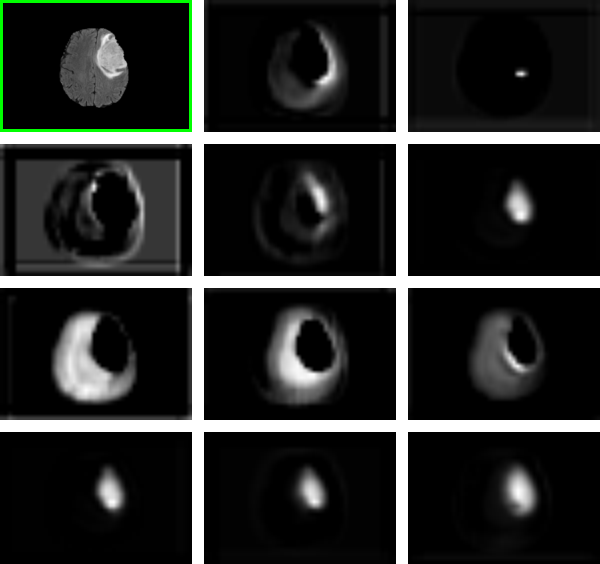
\includegraphics[height=6.2cm]{activation_maps/activations_ds09_0097}
  }
  \hfill
  \subfloat[Example on \textit{Slit-Lamp Retina B}]
  {
    \label{fig:subfig:activatiom_map_ds13}
    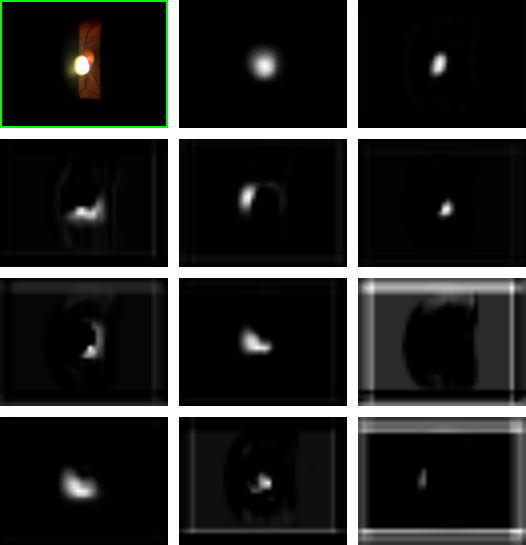
\includegraphics[height=6.2cm]{activation_maps/activations_ds13_0109}
  }
  \caption[Activation maps]{Activation maps of a trained \textit{U-Net Rec} model. The upper left image shows the passed image from (a) \textit{MRI Brain A}, and (b) \textit{Slit-Lamp Retina B} datasets. The other $11$ plots show some randomly chosen activation maps, extracted at the deepest level after the last ReLU.}
  \label{fig:activatiom_maps}
\end{figure}

\clearpage
\section{Feature Extracting Methods}
We provide results of the evaluation of our feature extraction methods. The evaluation procedure's configurations are first described. Second, the numerical values of the parameters of our methods are given. Third, we show the influence of using data augmentation. Fourth, we give experimental results on the feature performance vs. training-time. Fifth, the influence of the selected features of Random Forest is observed. Sixth, we present an overall ranking of the feature extraction methods in terms of \textit{max F1-Score}. Lastly, we investigate the influence of zero-padding.

\subsection{Configurations of Evaluation Procedure} \label{ch:eval_configs}
In chapter \ref{optimization} we stated that weight initialization of neural networks can be crucial for performance. Depending on the initialization, the gradient-based optimization will end in different minima and thus, might not be very constant. One could seed the random number generators, such that it always produces the same output. Anyhow, since we compare between different methods, seeding the random number generators would not allow a fair comparison.

U-Net based methods are evaluated in ten repetitions, i.e. each model is trained ten times on each dataset, resulting in ten different feature sets per dataset and method. We evaluate each feature matrix individually by the Random Forest classifier. Its settings are described in chapter \ref{random_forest}. For evaluation, the Random Forest is not seeded.

Concerning the baseline methods (including \textit{VGG-16}), the overall performance is largely unaffected by the random initialization. Thus, for those methods, we produced only one feature matrix per method and dataset. However, the Random Forest, in turn, is applied ten times on each feature matrix.

\subsection{Parameterization of Feature Extraction Methods}
We now give the numerical values of the parameters of our models. The parameters of the baseline methods are given first, followed by the U-Net based method's parameters. For detailed information on the methods, refer to chapter \ref{ch:methods}.

\subsubsection{Baseline Methods}
Tab. \ref{tab:baseline_params} shows the different parameters used for all baseline methods. For comparison purpose, both \textit{ScSP} and \textit{BoVW}, have $512$ classes and a SIFT keypoint size of $16 \times 16$ pixels. The number of keypoints used for vector quantization is defined in terms of number per image for the \textit{BoVW} method, and number over the entire sequence for the \textit{ScSP} method. We experimented with the patch size used for the \textit{ScSP} and \textit{VGG-16} methods. For \textit{ScSP}, taking the width as three times the average width of superpixels ($MSPW$) leads to best results. For the \textit{VGG-16} method, the optimal patch size is found to be two times the $MSPW$. We define:

\begin{equation}
   MSPW = \frac{1}{S} \sum_{i=1}^S \sqrt{A_i}
   \label{eq:mspw} 
\end{equation}
\vspace{6pt}

Where $S$ is the number of superpixels in the sequence and $A \in \mathbb{Z}$ the area of the individual superpixel measured in pixels. 

\clearpage
\begin{table}[!htbp]
   \centering
   \caption[Baseline parameters]{Illustration of parameters used in the baseline methods. The individual methods are described in chapter \ref{ch:baselines}.}
   \begin{tabular}{c|m{1.3cm}|c|l}
      \toprule
      \textbf{Method} & \textbf{Symbol} & \textbf{\makecell{Feature \\ Dimension $D$}} & \textbf{Parameters}\\
      \midrule
      BoVW & \makecell{
\includegraphics[width=1cm]{icons/bovw}} & $512$ & 
        \makecell[l]{Number of classes = $512$ \\ 
                  SIFT KP size = $16 \times 16$px \\
                  Number of KP for CB per image = $100$} \\
      \midrule
      ScSP & \makecell{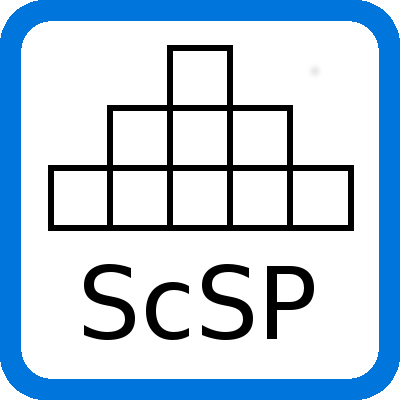
\includegraphics[width=1cm]{icons/scsp}} & $10'752$ & 
        \makecell[l]{Number of classes = $512$ \\ 
                  SIFT KP size = $16 \times 16$px \\
                  Number of KP for CB over all sequence = $20'000$ \\
                  Pyramid levels = $[1,2,4]$ \\
                  Patch width and height = $3 \cdot MSPW$} \\
      \midrule
      VGG-16 & \makecell{
\includegraphics[width=1cm]{icons/vgg}} & $4'096$ & 
        \makecell[l]{Patch width and height = $2 \cdot MSPW$} \\
      \bottomrule
      \multicolumn{4}{c}{KP $\coloneqq$ keypoint \hspace{14pt} CB $\coloneqq$ codebook \hspace{14pt} MSPW $\coloneqq$ mean superpixel width} \\
      \bottomrule
   \end{tabular}
   \label{tab:baseline_params}
\end{table}
\vspace{20pt}

\subsubsection{U-Net Based Methods}
Tab. \ref{tab:unet_params} give the values of the parameters of our U-Net based models. For methods that predict a probability map $\boldsymbol{\hat{Z}}$, we set $\sigma$ to $6\%$ of the image width. For methods that involve the probability map $\bm{Z}$ in their loss-functions, we set $\sigma$ to $30\%$ of the image width. Fig. \ref{fig:prob_maps} shows ($\boldsymbol{Z}/\max{\{\boldsymbol{Z}\}}$) with the two $\sigma$ values mentioned above.
\vspace{30pt}

\begin{table}[!htbp]
   \centering
   \caption[U-Net based method parameters]{Illustration of parameters used in the U-Net based methods.}
   \begin{tabular}{l|m{3.3cm}|l}
      \toprule
      \textbf{Method} & \textbf{\makecell{Symbol}} & \textbf{Parameters}\\
      \midrule
      U-Net Gaze Rec & \makecell{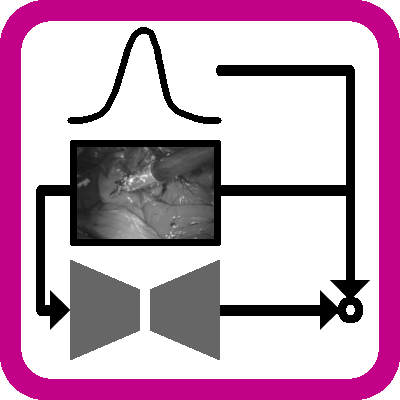
\includegraphics[width=1cm]{icons/unet_gaze_rec}} & 
        \makecell[l]{$\sigma = 30\%$ of image width} \\
      \midrule
        \makecell[l]{U-Net Gaze Prob \\
                     U-Net Gaze Prob Freeze \\
                     U-Net Gaze Prob Concat} & 
      \makecell{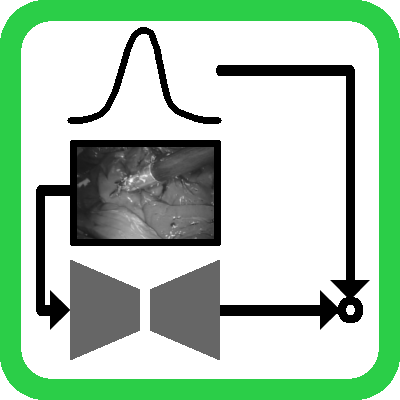
\includegraphics[width=1cm]{icons/unet_gaze_prob} 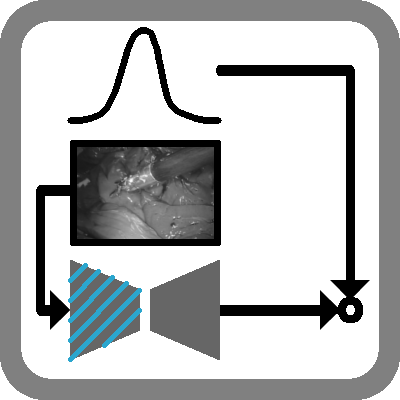
\includegraphics[width=1cm]{icons/unet_gaze_prob_freeze} \includegraphics[width=1cm]{icons/unet_gaze_prob_concat}} & 
        \makecell[l]{$\sigma = 6\%$ of image width} \\
      \midrule
      U-Net Gaze Prob LSTM & \makecell{\includegraphics[width=1cm]{icons/unet_gaze_prob_lstm}} & 
        \makecell[l]{$\sigma = 6\%$ of image width \\
                     $\alpha = 0.2$} \\  
      \bottomrule
   \end{tabular}
   \label{tab:unet_params}
\end{table}

\clearpage
\begin{figure}[!htbp]
  \centering
  \subfloat[$\sigma = 6\%$ of image width]
  {
    \includegraphics[width=6cm]{probability_maps/prob_map_06}
  }
  \hfill
  \subfloat[$\sigma = 30\%$ of image width]
  {
    \includegraphics[width=6cm]{probability_maps/prob_map_30}
  }
  \caption[Illustration of probability maps]{Visualization of probability map ($\boldsymbol{Z}/\max{\{\boldsymbol{Z}\}}$). In (a), we show the probability map for methods that predict $\boldsymbol{\hat{Z}}$. (b) shows the probability map of method \textit{U-Net Gaze Rec}.}
  \label{fig:prob_maps}  
\end{figure}

\subsection{Importance of Data Augmentation} \label{ch:nec_data_gen}
To explore the importance of data augmentation, we trained a \textit{U-Net Rec} model once with standard configuration (use of data generator) and once without using the data generator. As for all experiments, we performed the training and evaluation with ten repetitions, then took the mean \textit{max F1-Score}. We performed this experiment on one dataset per image modality. The results are summarized in Tab. \ref{tab:data_gen_nec}.
\vspace{30pt}

\begin{table}[!htbp]
   \centering
   \caption[Importance of data generator]{Influence of data augmentation in terms of mean \textit{max F1-Score} over ten repetitions. A \textit{U-Net Rec} model is trained in standard configuration, i.e. using data agumentation and without using data augmentation.}
   \begin{tabular}{l|*{4}{c|}}
      \toprule
       & \rotatebox[origin=cB]{90}{\parbox[t]{3.2cm}{\hspace{3pt} \textbf{Surgical Video} \hspace*{\fill}}} 
       & \rotatebox[origin=cB]{90}{\parbox[t]{3.2cm}{\hspace{3pt} \textbf{MRI Brain A} \hspace*{\fill}}} 
       & \rotatebox[origin=cB]{90}{\parbox[t]{3.2cm}{\hspace{3pt} \textbf{CT Inner Ear A} \hspace*{\fill}}} 
       & \rotatebox[origin=cB]{90}{\parbox[t]{3.2cm}{\hspace{3pt} \textbf{Slit-Lamp A} \hspace*{\fill}}} \\
      \midrule
      Data Augmentation \textbf{not in use} & 0.9826 & 0.9792 & 0.9587 & 0.9800 \\\midrule
      Data Augmentation \textbf{in use} & 0.9832 & 0.9810 & 0.9621 & 0.9863 \\\midrule\midrule
      \textbf{Gain} by using Data Augmentation & \textbf{0.061\%} & \textbf{0.184\%} & \textbf{0.355\%} & \textbf{0.643\%} \\
      \bottomrule
   \end{tabular}
   \label{tab:data_gen_nec}
\end{table}

\clearpage
\subsection{Performance w.r.t Training Time} \label{ch:perf_vs_training}
We now evaluate the performance of our features with respect to training time. We trained a \textit{U-Net Rec} model over $100$ epochs and evaluated features every $10$ epochs. Similar to all of our evaluations, we did the training and evaluation with ten repetitions to reduce variance. Fig. \ref{fig:perf_vs_training} shows the mean \textit{max F1-Score} for one dataset per image modality. We notice that past $20$ epochs the performance stagnates or even decreases in the case of the \textit{CT Inner Ear A} dataset. The next section provides more insight on that particular behaviour.
\vspace{30pt}

\begin{figure}[!htbp]
  \centering
  {
    \includegraphics[width=\textwidth]{f1_score_vs_training_time/f1_vs_training_rec}
  }
  \caption[Feature quality vs training time of U-Net Rec model]{Mean \textit{max F1-Score} over ten repetitions w.r.t training time. The graph shows the results of \textit{U-Net Rec} model for one dataset per image modality.}
  \label{fig:perf_vs_training}
\end{figure}

\clearpage
\subsection{Influence on Random Forest Feature Selection} \label{ch:ch_infl_feat_selection}
Fig. \ref{fig:perf_vs_training_maxfeat} shows a comparison of performances for dataset \textit{CT Inner Ear A} where we isolate the parameter $m$, the number of sampled features of the Random Forest (refer to chapter \ref{random_forest}). We observe that setting $m=\sqrt{p}$, as advised by \cite[Ch. 15]{Hastie2009}, gives higher \textit{max F1-Scores} compared to $m=p$.
Both curves show a decreasing tendency.
\vspace{10pt}
%\myworries{Also, the latter case overfits past $60$ epochs in contrast with $m=\sqrt{p}$ where overfitting happens earlier and is more progressive.}

\begin{figure}[!htbp]
  \centering
  {
    \includegraphics[width=\textwidth]{f1_score_vs_training_time/f1_vs_training_rec_maxfeat}
  }
  \caption[Feature quality vs training time of U-Net Rec model]{Mean \textit{max F1-Score} over ten repetitions w.r.t training time. The graph shows the results of \textit{U-Net Rec} model for dataset \textit{CT Inner Ear A}. The red curve illustrates the result when Random Forest selects $m=\sqrt{p}$ features and the cyan curve when selecting $m=p$.}
  \label{fig:perf_vs_training_maxfeat}
\end{figure}

Based on this observations, we choose to train our U-Net based models for $20$ epochs and set $m=\sqrt{p}$ in the following experiments.
\vspace{20pt}

\subsection{Method Comparison}
Tab. \ref{tab:final_results} summarizes the feature performance for each dataset and method in terms of \textit{max F1-Scores} averaged over ten repetitions. The standard deviation is given underneath each score. All best scores per dataset are marked in red font. For each dataset and method, we performed a two-sided Welch's t-test \cite{Welch1947} to test if the score reached by the individual method is significantly different to the score reached by the best method for that dataset. We used Welch's t-test since we have independent samples and unequal variances. All values marked in bold font are not significantly different to the best score for a significance level of $0.05$. The last row declares how many times the individual method did not significantly perform worse than the best method. We name this score \textit{Top-Sig-Score}.

\begin{table}[!htbp]
   \centering
   \caption[Feature quality]{Performance in terms of \textit{max F1-Scores} averaged over ten repetitions for each dataset and method, respectively. The according standard deviation is given underneath each score. Best scores per dataset are marked in red font. All bold marked scores are not significantly different from the best score when testing by a two-sided Welch's t-test with a significance level of 0.05. The last row shows on how many datasets the specific method was not significantly different to the best method.}
   \begin{tabular}{l|*{9}{c|}}
      \toprule
       & \rotatebox[origin=cB]{90}{\parbox[t]{4cm}{BoVW \hspace*{\fill}}} 
       & \rotatebox[origin=cB]{90}{\parbox[t]{4cm}{ScSP \hspace*{\fill}}} 
       & \rotatebox[origin=cB]{90}{\parbox[t]{4cm}{VGG \hspace*{\fill}}} 
       & \rotatebox[origin=cB]{90}{\parbox[t]{4cm}{U-Net Rec \hspace*{\fill}}} 
       & \rotatebox[origin=cB]{90}{\parbox[t]{4cm}{U-Net Gaze Rec \hspace*{\fill}}} 
       & \rotatebox[origin=cB]{90}{\parbox[t]{4cm}{U-Net Gaze Prob \hspace*{\fill}}} 
       & \rotatebox[origin=cB]{90}{\parbox[t]{4cm}{U-Net Gaze Prob Freeze \hspace*{\fill}}} 
       & \rotatebox[origin=cB]{90}{\parbox[t]{4cm}{U-Net Gaze Prob Concat \hspace*{\fill}}}
       & \rotatebox[origin=cB]{90}{\parbox[t]{4cm}{U-Net Gaze Prob LSTM \hspace*{\fill}}}  \\
       & \raisebox{-\totalheight}{\includegraphics[width=0.8cm]{icons/bovw}} 
       & \raisebox{-\totalheight}{\includegraphics[width=0.8cm]{icons/scsp}} 
       & \raisebox{-\totalheight}{\includegraphics[width=0.8cm]{icons/vgg}} 
       & \raisebox{-\totalheight}{\includegraphics[width=0.8cm]{icons/unet_rec}} 
       & \raisebox{-\totalheight}{\includegraphics[width=0.8cm]{icons/unet_gaze_rec}} 
       & \raisebox{-\totalheight}{\includegraphics[width=0.8cm]{icons/unet_gaze_prob}} 
       & \raisebox{-\totalheight}{\includegraphics[width=0.8cm]{icons/unet_gaze_prob_freeze}} 
       & \raisebox{-\totalheight}{\includegraphics[width=0.8cm]{icons/unet_gaze_prob_concat}} 
       & \raisebox{-\totalheight}{\includegraphics[width=0.8cm]{icons/unet_gaze_prob_lstm}}\\
      \midrule\midrule
      {\scriptsize Surgical Video} & \scriptsize 0.6649 & \scriptsize 0.8998 & \scriptsize 0.9647 & \textbf{\scriptsize 0.9830} & {\color{red} \textbf{\scriptsize 0.9832}} & \scriptsize 0.9791 & \scriptsize 0.9811 & \scriptsize 0.9776 & \scriptsize 0.9807 \\[-4pt]
       & \tiny $\pm$6.24e-4 & \tiny $\pm$6.04e-4 & \tiny $\pm$3.87e-4 & \tiny $\pm$4.84e-4 & \tiny $\pm$4.22e-4 & \tiny $\pm$1.84e-3 & \tiny $\pm$4.78e-4 & \tiny $\pm$2.93e-3 & \tiny $\pm$7.21e-4 \\\midrule\midrule
      {\scriptsize MRI Brain A} & \scriptsize 0.3163 & \scriptsize 0.9288 & \scriptsize 0.9666 & \textbf{\scriptsize 0.9774} & {\color{red} \textbf{\scriptsize 0.9810}} & \scriptsize 0.9764 & \textbf{\scriptsize 0.9806} & \scriptsize 0.9673 & \textbf{\scriptsize 0.9794} \\[-4pt]
       & \tiny $\pm$3.61e-3 & \tiny $\pm$5.05e-3 & \tiny $\pm$2.10e-3 & \tiny $\pm$4.65e-3 & \tiny $\pm$3.95e-3 & \tiny $\pm$3.30e-3 & \tiny $\pm$3.28e-3 & \tiny $\pm$8.90e-3 & \tiny $\pm$5.02e-3 \\\midrule
      {\scriptsize MRI Brain B} & \scriptsize 0.7502 & \scriptsize 0.8568 & \scriptsize 0.8911 & \textbf{\scriptsize 0.9232} & \textbf{\scriptsize 0.9292} & \scriptsize 0.9142 & \textbf{\scriptsize 0.9253} & {\color{red} \textbf{\scriptsize 0.9297}} & \scriptsize 0.9201 \\[-4pt]
       & \tiny $\pm$8.20e-3 & \tiny $\pm$7.36e-3 & \tiny $\pm$3.88e-3 & \tiny $\pm$5.63e-3 & \tiny $\pm$3.74e-3 & \tiny $\pm$8.59e-3 & \tiny $\pm$4.83e-3 & \tiny $\pm$7.09e-3 & \tiny $\pm$7.90e-3 \\\midrule
      {\scriptsize MRI Brain C} & \scriptsize 0.7911 & \scriptsize 0.8957 & \scriptsize 0.9345 & \textbf{\scriptsize 0.9766} & \textbf{\scriptsize 0.9742} & \scriptsize 0.9695 & {\color{red} \textbf{\scriptsize 0.9774}} & \textbf{\scriptsize 0.9742} & \scriptsize 0.9729 \\[-4pt]
       & \tiny $\pm$7.21e-3 & \tiny $\pm$2.66e-3 & \tiny $\pm$3.28e-3 & \tiny $\pm$3.75e-3 & \tiny $\pm$3.31e-3 & \tiny $\pm$2.96e-3 & \tiny $\pm$2.11e-3 & \tiny $\pm$5.15e-3 & \tiny $\pm$4.03e-3 \\\midrule
      {\scriptsize MRI Brain D} & \scriptsize 0.7035 & \scriptsize 0.7764 & \scriptsize 0.8548 & {\color{red} \textbf{\scriptsize 0.9470}} & \textbf{\scriptsize 0.9463} & \scriptsize 0.9207 & \scriptsize 0.9247 & \scriptsize 0.9293 & \scriptsize 0.9276 \\[-4pt]
       & \tiny $\pm$1.27e-2 & \tiny $\pm$6.67e-3 & \tiny $\pm$6.11e-3 & \tiny $\pm$5.42e-3 & \tiny $\pm$4.67e-3 & \tiny $\pm$5.48e-3 & \tiny $\pm$5.48e-3 & \tiny $\pm$4.51e-3 & \tiny $\pm$5.00e-3 \\\midrule
      {\scriptsize MRI Brain (B-D)} & \scriptsize 0.6753 & \scriptsize 0.8046 & \scriptsize 0.8640 & {\color{red} \textbf{\scriptsize 0.9482}} & \textbf{\scriptsize 0.9463} & \scriptsize 0.9167 & \scriptsize 0.9399 & \scriptsize 0.9236 & \scriptsize 0.9310 \\[-4pt]
       & \tiny $\pm$4.83e-3 & \tiny $\pm$1.67e-3 & \tiny $\pm$2.61e-3 & \tiny $\pm$4.65e-3 & \tiny $\pm$3.80e-3 & \tiny $\pm$1.30e-2 & \tiny $\pm$3.40e-3 & \tiny $\pm$5.42e-3 & \tiny $\pm$1.16e-2 \\\midrule\midrule
      {\scriptsize CT Inner Ear A} & \scriptsize 0.5527 & \scriptsize 0.8680 & \scriptsize 0.7400 & \textbf{\scriptsize 0.9624} & \textbf{\scriptsize 0.9621} & \scriptsize 0.9565 & \scriptsize 0.9554 & \textbf{\scriptsize 0.9660} & {\color{red} \textbf{\scriptsize 0.9686}} \\[-4pt]
       & \tiny $\pm$1.24e-2 & \tiny $\pm$1.02e-2 & \tiny $\pm$6.09e-3 & \tiny $\pm$4.75e-3 & \tiny $\pm$6.38e-3 & \tiny $\pm$8.60e-3 & \tiny $\pm$6.42e-3 & \tiny $\pm$7.20e-3 & \tiny $\pm$8.12e-3 \\\midrule
      {\scriptsize CT Inner Ear B} & \scriptsize 0.4659 & \scriptsize 0.8372 & \scriptsize 0.7786 & {\color{red} \textbf{\scriptsize 0.9628}} & \textbf{\scriptsize 0.9623} & \scriptsize 0.9481 & \scriptsize 0.9443 & \scriptsize 0.9560 & \scriptsize 0.9476 \\[-4pt]
       & \tiny $\pm$1.78e-2 & \tiny $\pm$5.55e-3 & \tiny $\pm$5.11e-3 & \tiny $\pm$3.34e-3 & \tiny $\pm$1.41e-3 & \tiny $\pm$7.64e-3 & \tiny $\pm$6.63e-3 & \tiny $\pm$4.61e-3 & \tiny $\pm$1.35e-2 \\\midrule\midrule
      {\scriptsize Slit-Lamp A} & \scriptsize 0.8912 & \scriptsize 0.9742 & \scriptsize 0.9784 & \textbf{\scriptsize 0.9845} & \textbf{\scriptsize 0.9863} & \scriptsize 0.9839 & {\color{red} \textbf{\scriptsize 0.9890}} & \scriptsize 0.9788 & \scriptsize 0.9780 \\[-4pt]
       & \tiny $\pm$9.97e-3 & \tiny $\pm$5.34e-3 & \tiny $\pm$3.57e-3 & \tiny $\pm$5.20e-3 & \tiny $\pm$3.36e-3 & \tiny $\pm$4.06e-3 & \tiny $\pm$2.74e-3 & \tiny $\pm$8.12e-3 & \tiny $\pm$4.20e-3 \\\midrule
      {\scriptsize Slit-Lamp B} & \scriptsize 0.6454 & \textbf{\scriptsize 0.9909} & \scriptsize 0.9775 & \scriptsize 0.9687 & \scriptsize 0.9747 & \textbf{\scriptsize 0.9888} & \scriptsize 0.9707 & {\color{red} \textbf{\scriptsize 0.9913}} & \scriptsize 0.9827 \\[-4pt]
       & \tiny $\pm$1.29e-2 & \tiny $\pm$2.48e-3 & \tiny $\pm$4.05e-3 & \tiny $\pm$8.44e-3 & \tiny $\pm$6.62e-3 & \tiny $\pm$4.32e-3 & \tiny $\pm$5.33e-3 & \tiny $\pm$2.43e-3 & \tiny $\pm$4.05e-3 \\\midrule
      {\scriptsize Slit-Lamp C} & \scriptsize 0.8681 & {\color{red} \textbf{\scriptsize 0.9870}} & \scriptsize 0.9724 & \textbf{\scriptsize 0.9862} & \textbf{\scriptsize 0.9826} & \scriptsize 0.9686 & \textbf{\scriptsize 0.9792} & \scriptsize 0.9736 & \scriptsize 0.9707 \\[-4pt]
       & \tiny $\pm$5.63e-3 & \tiny $\pm$3.43e-3 & \tiny $\pm$4.55e-3 & \tiny $\pm$7.43e-3 & \tiny $\pm$5.50e-3 & \tiny $\pm$1.33e-2 & \tiny $\pm$8.54e-3 & \tiny $\pm$9.44e-3 & \tiny $\pm$7.07e-3 \\\midrule
      {\scriptsize Slit-Lamp D} & \scriptsize 0.7752 & \scriptsize 0.9837 & \scriptsize 0.9460 & \textbf{\scriptsize 0.9874} & \scriptsize 0.9852 & \scriptsize 0.9764 & {\color{red} \textbf{\scriptsize 0.9918}} & \scriptsize 0.9800 & \scriptsize 0.9780 \\[-4pt]
       & \tiny $\pm$8.40e-3 & \tiny $\pm$2.03e-3 & \tiny $\pm$3.89e-3 & \tiny $\pm$6.05e-3 & \tiny $\pm$6.03e-3 & \tiny $\pm$1.16e-2 & \tiny $\pm$4.18e-3 & \tiny $\pm$5.49e-3 & \tiny $\pm$3.84e-3 \\\midrule
      {\scriptsize Slit-Lamp (A-D)} & \scriptsize 0.7663 & \scriptsize 0.9729 & \scriptsize 0.9507 & \textbf{\scriptsize 0.9779} & {\color{red} \textbf{\scriptsize 0.9785}} & \scriptsize 0.9669 & \textbf{\scriptsize 0.9767} & \scriptsize 0.9715 & \scriptsize 0.9641 \\[-4pt]
       & \tiny $\pm$9.04e-3 & \tiny $\pm$1.41e-3 & \tiny $\pm$2.57e-3 & \tiny $\pm$3.32e-3 & \tiny $\pm$3.19e-3 & \tiny $\pm$1.10e-2 & \tiny $\pm$3.22e-3 & \tiny $\pm$6.59e-3 & \tiny $\pm$5.98e-3 \\\bottomrule\toprule
      {\scriptsize \textbf{Top-Sig-Score}} & 0 & 2 & 0 & 12 & 11 & 1 & 7 & 4 & 2 \\\bottomrule
   \end{tabular}
   \label{tab:final_results}
\end{table}

Surprisingly, one baseline method (\textit{ScSP}) reached two times the \textit{Top-Sig-Score}. Both times in a slit-lamp sequence. Fig. \ref{fig:curves_ds14} gives detailed results on the \textit{Slit-Lamp Retina C} dataset. Fig. \ref{subfig:pr_curve_ds14} shows the PR-Curve as an average over all ten repetitions. Fig. \ref{subfig:reprod_ds14} illustrates the distribution of the \textit{max F1-scores} over ten repetitions as a box-plot.

Similarly to Fig. \ref{fig:curves_ds14}, we show in Fig. \ref{fig:curves_ds16} detailed results of dataset \textit{MRI Brain B} to illustrate the improvement obtained by U-Net based methods on that image modality.

\begin{figure}[!htbp]
  \centering
  \subfloat[\textit{PR-Curves} of dataset \textit{Slit-Lamp Retina C} with an example image]
  {
    \label{subfig:pr_curve_ds14}
    \includegraphics[width=12cm]{final_eval/ds14_pr}
  }
  \\[30pt]
  \subfloat[\textit{Max F1-Scores} of dataset \textit{Slit-Lamp Retina C}]
  {
    \label{subfig:reprod_ds14}
    \includegraphics[width=10cm]{final_eval/ds14_reprod}
  }
  \caption[Detailed results of dataset \textit{Slit-Lamp Retina C}]{Detailed results of dataset \textit{Slit-Lamp Retina C}. (a) \textit{PR-Curves} averaged on ten repetitions. \textit{Max F1-Scores} are given in the legends. (b) Box-plot of \textit{max F1-Score} on each repetition. The median is drawn in orange.}
  \label{fig:curves_ds14}  
\end{figure}

\clearpage
\begin{figure}[!htbp]
  \centering
  \subfloat[\textit{PR-Curves} of dataset \textit{MRI Brain B} with an example image]
  {
    \includegraphics[width=12cm]{final_eval/ds16_pr}
  }
  \\[20pt]
  \subfloat[\textit{Max F1-Scores} of dataset \textit{MRI Brain B}]
  {
    \includegraphics[width=10cm]{final_eval/ds16_reprod}
  }
  \caption[Detailed results of dataset \textit{Slit-Lamp Retina C}]{Detailed results of dataset \textit{MRI Brain B}. (a) \textit{PR-Curves} averaged on ten repetitions. \textit{Max F1-Scores} are given in the legends. (b) Box-plot of \textit{max F1-Score} on each repetition. The median is drawn in orange.}
  \label{fig:curves_ds16}  
\end{figure}

\subsection{Zero-Padding vs. Symmetric-Padding} \label{ch:zero_vs_sym_pad}
To investigate the influence of the border-effect due to zero-padding, we retrained our best model \textit{U-Net Gaze Rec} using symmetric-padding for all convolutional layers. When padding the input with symmetric property, the added pixel rows and columns are a mirror reflection of the input itself. We trained the model on one dataset per image modality. Fig. \ref{fig:activatiom_maps_sym} shows the activation maps of (a) zero-padding and (b) symmetric-padding on \textit{MRI Brain A}. The features are extracted from the last ReLU of the deepest level (see chapter \ref{ch:act_maps}).

\begin{figure}[!htbp]
  \centering
  \subfloat[Activation maps with zero-padding]
  {
    \includegraphics[height=5.8cm]{activation_maps/activations_ds09_0097_gaze_rec}
  }
  \hfill
  \subfloat[Activation maps with symmetric-padding]
  {
    \includegraphics[height=5.8cm]{activation_maps/activations_ds09_0097_gaze_rec_sympadded}
  }
  \caption[Activation maps symmetric padding]{Activation maps of a trained \textit{U-Net Gaze Rec} model with (a) zero-padding (standard configuration) and (b) symmetric-padding for the convolutional layers. The upper left image shows the passed image from \textit{MRI Brain A} datasets. The other $11$ plots show some randomly chosen activation maps, extracted at the deepest level after the last ReLU.}
  \label{fig:activatiom_maps_sym}
\end{figure}

In Tab. \ref{tab:zero_vs_sym_padd} we show the mean \textit{max F1-Scores} over ten repetitions for zero-padding (standard configuration) and symmetric-padding. There is no improvement observed.

\begin{table}[!htbp]
   \centering
   \caption[Zero vs. symmetric padding]{Comparison of zero-padding vs. symmetric-padding of the convolutional layers on a \textit{U-Net Gaze Rec} model. The values show the feature quality in terms of mean \textit{max F1-Scores} for one dataset per image modality over ten repetitions. The last column indicates the improvement due to symmetric-padding.}
   \small
   \begin{tabular}{l|c|c||c|}
      \toprule
       & \Gape[6pt][6pt]{\rotatebox[origin=cB]{90}{\parbox[t]{2.6cm}{U-Net Gaze Rec \\ \textit{\textbf{Zero-Pad}\hspace*{\fill}}}}}
       & \rotatebox[origin=cB]{90}{\parbox[t]{2.6cm}{U-Net Gaze Rec \\ \textit{\textbf{Symmetric-Pad}\hspace*{\fill}}}}
       & \rotatebox[origin=cB]{90}{\parbox[t]{2.6cm}{\textbf{Improvement\hspace*{\fill}}}} \\
      \midrule
      \textbf{Surgical Video} & 0.9832 & 0.9823  & \textbf{-0.091\%} \\\midrule
      \textbf{MRI Brain A} & 0.9810 & 0.9830 &  \textbf{+0.203\%} \\\midrule
%      {\scriptsize MRI Brain B} & \scriptsize 0.9292 & \scriptsize 0.9278 & \scriptsize -0.0014 \\\midrule
%      {\scriptsize MRI Brain C} & \scriptsize 0.9742 & \scriptsize 0.9760 & \scriptsize +0.0018 \\\midrule
%      {\scriptsize MRI Brain D} & \scriptsize 0.9463 & \scriptsize 0.9470 & \scriptsize +0.0006 \\\midrule
%      {\scriptsize MRI Brain (B-D)} & \scriptsize 0.9463 & \scriptsize 0.9431 & \scriptsize -0.0032 \\\midrule\midrule
      \textbf{CT Inner Ear A} & 0.9621 & 0.9535 & \textbf{-0.893\%} \\\midrule
%      {\scriptsize CT Inner Ear B} & \scriptsize 0.9623 & \scriptsize 0.9566 & \scriptsize -0.0057 \\\midrule\midrule
      \textbf{Slit-Lamp A} & 0.9863 & 0.9860 & \textbf{-0.03\%} \\
%      {\scriptsize Slit-Lamp B} & \scriptsize 0.9747 & \scriptsize 0.9796 & \scriptsize +0.0049 \\\midrule
%      {\scriptsize Slit-Lamp C} & \scriptsize 0.9826 & \scriptsize 0.9846 & \scriptsize +0.002 \\\midrule
%      {\scriptsize Slit-Lamp D} & \scriptsize 0.9852 & \scriptsize 0.9886 & \scriptsize +0.0034 \\\midrule
%      {\scriptsize Slit-Lamp A-D} & \scriptsize 0.9785 & \scriptsize 0.9763 & \scriptsize -0.0022 \\
      \bottomrule
   \end{tabular}
   \label{tab:zero_vs_sym_padd}
\end{table}

%%% Local Variables:
%%% mode: latex
%%% TeX-master: "../../main"
%%% End:

\resetfigpath{3-feats}

\chapter{Feature Extraction}
\label{ch:methods}
This chapter first describes the dataset modalities and properties. Second, we give an overview of our pipeline from training to evaluation. Third, we introduce the proposed methods for feature learning as well as the evaluation scheme. Concerning the feature representation learning, we first introduce our baseline methods, followed by the U-Net based methods.

Tab. \ref{tab:dataset_stat} summarizes the 13 datasets. We used four different MRI brain sequences (A-D). To augment the number of images for one dataset, the last three datasets (B-D) are combined into one larger dataset \textit{MRI Brain (B-D)}. In a similar manner, dataset \textit{Slit-Lamp Retina (A-D)} is constructed from concatenating four independent datasets together. The two independent datasets of the inner ear CT could not be concatenated due to different image resolutions. To each dataset, we also have corresponding xy-coordinates of the gaze location.

\begin{table}[ht]
   \centering
   \caption[Dataset statistics]{Summary and statistics of used datasets. Note the variety in size, resolution and color space.}
   \begin{tabular}{l|c|c|c|c|c}
      \toprule
      \textbf{Name} & \textbf{Size $N$} & \textbf{Height $H$ [px]} & \textbf{Width $W$ [px]} & \textbf{\#Channels $C$} \\
      \midrule
      Surgical Video Sequence & 1125 & 576 & 720 & 3 - RGB \\
      \midrule
      MRI Brain A & 129 & 540 & 782 & 1 - Gray \\
      MRI Brain B & 69 & 512 & 680 & 1 - Gray \\
      MRI Brain C & 75 & 512 & 680 & 1 - Gray \\
      MRI Brain D & 75 & 512 & 680 & 1 - Gray \\
      MRI Brain (B-D) & 219 & 512 & 680 & 1 - Gray \\
      \midrule
      CT Inner Ear A & 96 & 191 & 252 & 1 - Gray \\
      CT Inner Ear B & 99 & 290 & 300 & 1 - Gray \\
      \midrule
      Slit-Lamp Retina A & 194 & 512 & 680 & 3 - RGB \\
      Slit-Lamp Retina B & 121 & 512 & 680 & 3 - RGB \\
      Slit-Lamp Retina C & 75 & 512 & 680 & 3 - RGB \\
      Slit-Lamp Retina D & 130 & 512 & 680 & 3 - RGB \\
      Slit-Lamp Retina (A-D) & 520 & 512 & 680 & 3 - RGB \\
      \bottomrule
   \end{tabular}
   \label{tab:dataset_stat}
\end{table}

\section{Framework} \label{framework}
Fig. \ref{fig:Framework} illustrates our feature learning and evaluation framework. The individual blocks, such as superpixel segmentation, feature learning methods, and evaluation method, are elaborated in subsequent chapters. 

\begin{figure}[!htpb]
  \centering
  \includegraphics[width=13cm]{framework/framework}
  \caption[Framework description]{Framework description and how the individual parts are connected. Out of image data, superpixel segmentation and possible gaze locations, the feature learning algorithm construct a feature matrix $\boldsymbol{X}$, describing each superpixel by a feature. A Random Forest binary classifier is then trained and validated to make predictions of every superpixel. The labels are denoted by $\boldsymbol{y}$, describing if a superpixel belongs to foreground or background. At the bottom-right, we measure the performance of the classifier.}
  \label{fig:Framework}
\end{figure}

Performance evaluation of the different feature learning methods is done on a superpixel level. Hence, the feature learning methods shall output a feature vector for each of the superpixels. Refer to chapter \ref{superpixel_segm} for more details about the superpixel segmentation.

Let $N$ be the number of images in a data sequence and $S$ the number of superpixels over all sequence. As an example, if we have exactly $200$ superpixels per image, we would have $S=N \cdot 200$ superpixels in that sequence. To every superpixel, we want to assign a feature vector of dimension $D$. We can write the sequence feature matrix as $\boldsymbol{X} = [\boldsymbol{x}_1,...,\boldsymbol{x}_S]^T \in \mathbb{R}^{S \times D}$. Let $\boldsymbol{y} = [y_1,...y_S]^T \in \{0,1\}^S$ be the labels, meaning that $y_i=1$ for superpixels that count to the object of interest and $y_i=0$ for superpixels belonging to the background. Using the feature matrix $\boldsymbol{X}$ and the label vector $\boldsymbol{y}$, a random forest classifier then calculates performance measures, such as Precision-Recall curve and \textit{max F1-Score}. How the Random Forest classifier is applied is described in chapter \ref{random_forest}.

Some feature learning methods use the gaze location as an object prior, given as xy-coordinates for each image frame. The green point in Fig. \ref{fig:Framework} illustrates this location.

\section{Superpixel Segmentation} \label{superpixel_segm}
As described above, the performance evaluation is performed on a superpixel level. Having a feature vector for each superpixel instead of each pixel reduces the computational requirements. 

We used the superpixel segmentation algorithm ASLIC developed by Achanta et al. \cite{achanta12}.
SLIC stands for \textit{simple linear iterative clustering} and ASLIC for \textit{adaptive} SLIC. It relies on k-means clustering performed in color and spatial space. A trade-off between color similarity and spatial proximity is found necessary. In the SLIC approach, the problem is solved by using a compactness parameter. For images with both, flat and very textured regions, using the same compactness parameter lead to smooth regular-sized superpixel in the flat regions and highly irregular sized superpixel in textured regions. Thus, Achanta et al. invented the ASLIC approach, which adaptively chooses the compactness parameter for each superpixel differently. Fig. \ref{fig:ExSuperpixel} shows an example of using ASLIC on dataset \textit{Slit-Lamp Retina A}.

\begin{figure}[!htbp]
  \centering
  \label{fig:subfig:example_superpixel}
  \includegraphics[width=3.5cm]{superpixel_examples/ds12_superpixel}
  \caption[Example of superpixel segmentation]{Example of ASLIC superpixel segmentation on dataset \textit{Slit-Lamp Retina A} with number of superpixels $S=200$. Note the regular shape of superpixels in all regions.}
  \label{fig:ExSuperpixel}
\end{figure}

As parameter, the number of superpixels is crucial. In terms of trade-off, setting a large value will capture the contours of objects more accurately, at the cost of having a higher quantity of samples to predict/classify. We verified that taking $200$ superpixels per frame produces reasonably good segmentation on all our sequences.

Having at disposal ground truth data at pixel-level, we set the values of the output variable $\boldsymbol{y}$ the following way.
If one superpixel is covered by the ground truth pixel-wise segmentation by more than $50\%$ of its area, this specific superpixel is assigned to the foreground. Otherwise, it is assigned to the background.

\section{Feature Learning: Baselines} \label{ch:baselines}
To evaluate the performance of a method, a standard approach is to compare it to baseline methods. We used three different methods as baselines. The first method is called \textit{Bag of Visual Words (BoVW)}. A variant of the \textit{BoVW} approach is presented in a second baseline approach, so called \textit{Sparse Coded Spatial Pyramid (ScSP)}. This method is currently used in the superordinate project and therefore of high importance. The last baseline method follows the idea of transfer learning and uses a pre-trained VGG-16 network.

\subsection{Bag of Visual Words} \label{bow}
\begingroup
\setlength\intextsep{0pt}
\begin{wrapfigure}[4]{l}[0pt]{1.4cm}
\includegraphics[height=1.5cm]{icons/bovw}
\end{wrapfigure}

Bag of Visual Words (\textit{BoVW}), or Bag of Visual Features, is an unsupervised feature encoding method successfully utilized in scene classification \cite{zhang15}.
The algorithm can be split into feature learning and feature encoding phase \cite{cheriyadat14}. Feature learning phase is illustrated in Fig. \ref{fig:subfig:bow_training}. We developed a \textit{BoVW} approach where we choose the keypoints randomly over all images in a dataset. Each keypoint is then described by a SIFT descriptor of dimension 128. Subsequently, k-means vector quantization quantizes the keypoint descriptors into $K$ classes. Let $\boldsymbol{F} = [\boldsymbol{f}_1,...,\boldsymbol{f}_M]^T \in \mathbb{R}^{M \times 128}$ be the SIFT appearance descriptor of the $M$ keypoints. Eq. \ref{eq:k_means} describes the k-means objective function, where $\boldsymbol{C} = [\boldsymbol{c}_1,...,\boldsymbol{c}_K]^T \in \mathbb{R}^{K \times 128}$ denotes the codebook.

\endgroup

\begin{equation}
   \min_{\boldsymbol{C}} \sum_{m=1}^M \min_{k=1...K} \|\boldsymbol{f}_m - \boldsymbol{c}_k\|^2
   \label{eq:k_means} 
\end{equation}
\vspace{6pt}

The coding phase, shown in Fig. \ref{fig:subfig:bow_coding}, consists of describing each pixel by a SIFT descriptor and assigning it to the class whose centroids is the closest in terms of Euclidean distance. Subsequently, the assigned classes of every pixel in one superpixel are described in a histogram of $K$ bins. This results in a feature matrix of all superpixels in a sequence being $\boldsymbol{X} = [\boldsymbol{x}_1,...,\boldsymbol{x}_S]^T \in \mathbb{R}^{S \times D}$, where $D = K$. Extraction of the SIFT descriptors is done on grayscale data.

For SIFT extraction we used the OpenCV \cite{openCV} package with Python interface and k-means vector quantization is performed using SciPy's \cite{scipy} clustering tools.

\begin{figure}[htbp]
  \centering
  \subfloat[BoVW feature learning phase]
  {
    \label{fig:subfig:bow_training}
    \includegraphics[width=10cm]{bovw/bow_approach_training}
  }
  \\
  \subfloat[BoVW feature encoding phase]
  {
    \label{fig:subfig:bow_coding}
    \includegraphics[width=11cm]{bovw/bow_approach_coding}
  }
  \caption[BoVW illustration]{Illustration of \textit{BoVW} approach, divided in two phases. (a) shows the feature learning phase, where SIFT descriptors of randomly chosen keypoints are quantized into a codebook. In the encoding phase (b), each pixel is described by a SIFT descriptor and assigned to a class using the codebook. Subsequently, for each superpixel, a histogram of all assigned classes is created, which makes up the final feature descriptor.}
  \label{fig:BoVW_approch}  
\end{figure}

\subsection{Sparse Coded Spatial Pyramid} \label{scp}
\begingroup
\setlength\intextsep{0pt}
\begin{wrapfigure}[4]{l}[0pt]{1.4cm}
\includegraphics[height=1.5cm]{icons/scsp.png}
\end{wrapfigure}

Another baseline approach, called Sparse-coded Spatial Pyramid (\textit{ScSP}), can be seen as an improved version of the \textit{BoVW} approach with two main modifications. Firstly, instead of using standard k-means clustering, it uses sparse codes of SIFT features, and secondly, a pyramid representation is used. The following describes the added value of \textit{ScSP} with \textit{BoVW}.

\endgroup

%Max pooling instead of standard mean-statistics is not treated [well you just did it... cut and paste that somewhere relevant].

Mathematically, the objective of sparse coding for vector quantization can be written using matrix computation as shown in Eq. \ref{eq:sparse_codes}. The formulations below are adapted from Yang et al. \cite{yang09}.

\begin{samepage}
\begin{equation}
  \min_{\boldsymbol{U,C}} \sum_{m=1}^M \|\boldsymbol{f}_m - \boldsymbol{u}_m \boldsymbol{C}\|^2 + \lambda |\boldsymbol{u}_m|
  \label{eq:sparse_codes} 
\end{equation}
\begin{align*}
  \textrm{subject to } \|\boldsymbol{c}_k\| \leq 1, \hspace{6pt} \forall{k} = 1,2,...,K
\end{align*}
\end{samepage}

Similar to Eq. \ref{eq:k_means}, $\boldsymbol{f_m}$ represents the SIFT appearance vector of keypoint $m$ and $\boldsymbol{C}$ represents the codebook. $\boldsymbol{U} = [\boldsymbol{u}_1,...,\boldsymbol{u}_M]^T \in \mathbb{R}^{M \times K}$ defines the cluster membership indicator. The L2-norm on $\boldsymbol{c}_k$ is typically applied to avoid trivial solutions. If we drop the regularization term $\lambda |\boldsymbol{u}_m|$ and add a cardinality constraint to $\boldsymbol{u}_m$, meaning that only one element in $\boldsymbol{u}_m$ must be nonzero and positive, the sparse coding formulation in Eq. \ref{eq:sparse_codes} simplifies to k-means objective. Yang et al. \cite{yang09} approved that, compared to standard k-means coding, sparse coding can achieve a much lower reconstruction error due to less restrictive constraints. Sparsity also allows the representation to be specialized and capture salient properties of the image.

Lazebnik et al. \cite{lazebnik09} describe the spatial pyramid as a "collection of orderless feature histograms computed over cells defined by a multi-level recursive image decomposition". Fig. \ref{fig:pyramid_repr} show histograms extracted at different locations on an image. The final histogram representation is a concatenation of all histograms from all regions. After normalization, the concatenated histograms can again be seen as a histogram representing the full feature vector. Hence, for the example shown in Fig. \ref{fig:pyramid_repr} using pyramid levels $\boldsymbol{l} = [1,2,4]$, we have a feature dimension $D = K \cdot (1^2 + 2^2 + 4^2) = K \cdot 21$, where $K$ is the number of classes.

\begin{figure}[htbp]
  \centering
  \includegraphics[width=6cm]{scp/pyramid_representation}
  \caption[Spatial pyramid representation]{Illustration of the spatial pyramid representation. Histograms are computed at different levels which are then concatenated into one big vector. After normalization, this vector can again be seen as a histogram vector.}
  \label{fig:pyramid_repr}
\end{figure}

Using a pyramid representation implies that the image patch needs to be square. Intuitively, one wants to enclose within the patch some visual context around the superpixel region. We refer to this parameter as patch size.
In practice, we train our codebook in a similar fashion to \textit{BoVW}, i.e. convert images to grayscale and randomly sample keypoints on every image of the sequence. Each keypoint then gives a SIFT feature vector. Once trained, we extract squared patches of dimension centered on each superpixel's centroid location. We used the implementation of \cite{imdescrip}.

\subsection{VGG-16 Pretrained} \label{vgg}
\begingroup
\setlength\intextsep{0pt}
\begin{wrapfigure}[4]{l}[0pt]{1.4cm}
\includegraphics[height=1.5cm]{icons/vgg.png}
\end{wrapfigure}

VGGNet is a CNN for large-scale image recognition proposed by Simonyan and Zisserman \cite{simonyan15}.
Their work was submitted to the ImageNet \cite{ILSVRC15} Challenge 2014 (ILSVRC-2014) where they secured the first and second places in the localization and classification task, respectively.
Transferring pre-trained VGGNets to other tasks has been successfully used by Long et al.
\cite{long15} in semantic segmentation and Ng et al. \cite{ng15} in emotion recognition. Those successes motivated us to evaluate the performance of using a pre-trained VGGNet. However, we did not follow any fine tuning steps.

\endgroup

Simonyan and Zisserman \cite{simonyan15} proposed various network models.
We used a model with 16 weight layers and $3 \times 3$ convolution strides, described as configuration D \cite[Tab. 1]{simonyan15}.
This model was trained on the ILSVRC-2014 dataset and weights are available online \cite{simonyan14a}.
We took advantage of an already existing implementation by F. Chollet in Keras \cite{Keras}.
Similar to the \textit{ScSP} approach, we extracted patches at superpixel centroids and fed it to the network.
Since the input dimension of the network is fixed ($244 \times 244 \times 3$), our input data needed to be scaled to that size.
Resizing is done using bicubic interpolation method of Python's SciPy \cite{scipy} package.
The features are then extracted from the penultimate fully-connected layer, resulting in a feature dimension of $D=4096$.

From a theoretical point of view, let us mention that most machine learning methods make the assumption that training and unseen data lie in the same feature space and have a similar distribution.
However, in many real-world applications, this assumption may not hold, as stated by Pan et al. \cite{pan2010}.
In a setup where the training data largely differs (in the latter sense) from the data used for prediction, we talk about "Transfer Learning". We assume that a network pre-trained on a very large-scale dataset with high generalization will produce good features for our task.

\section{Feature Learning: U-Net Based} \label{ch:unet_based}
We now describe our U-Net based feature extraction methods. We first explain the architecture of the "core" model, i.e. one that will be modified to account for different outputs and loss functions. We dedicate the second section to data augmentation. The third section describes how the features can be extracted from the CNN model to obtain feature vectors. Our various modified U-Nets will then be described in detail. Finally, an overview summarizes all U-Net based methods.

\subsection{Core Model} \label{model}
Our CNN is a slight modification of the original U-Net structure described in chapter \ref{u_net}. We did not use the U-Net for image segmentation, as initially done by Ronneberger et. al. Instead, we trained the network in an unsupervised manner, like an autoencoder, on our data and extracted features at the lowest level. Some of our methods operate in a weakly-supervised fashion, where information related to the gaze location is used as a prior.

Fig. \ref{fig:unet_model} shows a modified U-Net structure. Similar to the original structure, we used two stacked convolution layers with $3 \times 3$ filter size and stride $1$ per level. Since we want the output to be the same size as the input, we used zero padding instead of valid padding. Thus, we modified the structure by adding a batch normalization layer with ReLU activation after the convolutional layers. Configurations of max-pooling did not change. Instead of using up-convolutional layers in the expansive path, we used upsampling layers, which apply a simple nearest neighbor interpolation to increase the resolution.

As shown in \cite{vorontsov17}, this last modification improves prediction performances.  In addition, upsampling layers are parameter-free and allow to reduce the memory requirement. The very last layer is a convolutional layer with filter size $1 \times 1$ and sigmoid activation. That our output value is between $0$ and $1$ is assured by the use of a last sigmoid activation layer.

In contrast with our baseline approaches, our U-Net methods take as input the full image instead of patches.
How the features are then assigned to the individual superpixel is described in chapter \ref{feat_extract}.
Max pooling downscales the resolution by $2$. Thus, the lowest resolution at the deepest layer is given by the input resolution divided by $2^4=16$. This implies that input image resolution must be dividable by 16. Hence, input images were downscaled to the nearest width and height which are dividable by $16$ before fed to the network. The number of input, as well as output channels, differ between the individual U-Net methods. In what follows, we refer to $c\_i$ as the number of input channels and $c\_o$ as the number of output channels. We normalized the inputs to have zero mean and a variance of $1$.

The use of batch normalization layers helps for optimization, as shown in chapter \ref{optimization}.
Since GPU memory is limited and data input resolution is rather large, we are restricted to small mini-batch sizes.
According to Gastaldi et al. \cite{gastaldi17}, batch normalization also has a regularization effect due to fluctuations in mini-batch statistics. Especially with small mini-batches, those fluctuations regularize the network.

\clearpage
\begin{figure}[!htbp]
  \centering
  \includegraphics[width=\textwidth]{unet/model5}
  \caption[Modified U-Net architecture]{Illustration of our modified U-Net structure. Other than the original U-Net structure, it has a batch normalization layer after each convolutional layer. Depending on the data color space and loss function, it uses different number of input channels $c\_i$ and output channels $c\_o$.}
  \label{fig:unet_model}
\end{figure}

\subsection{Data Augmentation} \label{ch:data_gen}
Since the datasets we used are rather small in size, we used data augmentation wherever possible to increase the training data size. However, since we have a setting where we train the neural network on the same data we later extract the features from, the model does not need to generalize to non-seen data. Hence, we only use image transforms that are observed within the data. For example, it is very likely that during a slit-lamp recording the user rotates and shifts the camera, resulting in different angles and positions of the optical disc. This confirms to use horizontal and vertical shift, as well as rotation for image transforms. Contrarily, as the size of the object seldom changes, scaling and zooming are not relevant transformations.
The same reasoning applies to other datasets.
To sum up, we resort to rotation, vertical/horizontal translation as well as little shearing. Additionally, we added Gaussian noise for regularization. In our implementation, we used the online data generator provided by the Keras framework \cite{Keras}, which randomly generates new data during training time. Some examples and parameters used are described in chapter \ref{results_data_gen}.

\clearpage
\subsection{Feature Extraction} \label{feat_extract}
Similarly to our baseline methods, U-Net based methods construct a feature matrix $\boldsymbol{X} = [\boldsymbol{x}_1,...,\boldsymbol{x}_S]^T \in \mathbb{R}^{S \times D}$ describing each superpixel. Fig. \ref{fig:feat_extract} illustrates this process on an example of a single image. After training, a forward pass is performed on all image and features are taken as the output (ReLU) of the deepest layer. Those features correspond to a downscaled version of the input image. Hence, it must be upscaled to the original image resolution. Each feature dimension is independently upscaled to the original image size using bicubic interpolation. Since one pixel becomes a region, extrapolation is also needed at border regions, shown by the red circle and square in Fig. \ref{fig:feat_extract}. As we now have a descriptor for each pixel upscaled to the same resolution as the original data, we can take the mean over all descriptors belonging to the individual superpixels with feature dimension $D=512$.
\vspace{10pt}

\begin{figure}[htbp]
  \centering
  \includegraphics[width=\textwidth]{feat_extract/feature_extraction}
  \caption[Feature extraction model]{Illustration of feature extraction for U-Net based methods. The features are extracted from the deepest level. Those features are then interpolated (and extrapolated) on each dimension individually to obtain the original resolution. Each pixel is described by a feature vector of dimension $D=512$.
    Superpixels are assigned to the mean of all feature vectors that it envelopes.}
  \label{fig:feat_extract}
\end{figure}

\subsection{U-Net Reconstruct}
\begingroup
\setlength\intextsep{0pt}
\begin{wrapfigure}[4]{l}[0pt]{1.4cm}
\includegraphics[height=1.5cm]{icons/unet_rec.png}
\end{wrapfigure}

\textit{U-Net Reconstruct} (or \textit{U-Net Rec}) is an unsupervised model. It takes as input the image data and reconstructs the same data. Let $\mathcal{I}$ be the image set and $\boldsymbol{I}_k \in [0,1]^{H \times W \times C}$ an image with height $H$, width $W$ and number of channels $C$. We assume that $\boldsymbol{I}_k$ is already downscaled to have $H$ and $W$ dividable by $16$ (see chapter \ref{model}). Pixels are described by $\boldsymbol{I}_k(i,j,c) \in [0,1]$ with $i$ and $j$ its indices. The reconstructed image, of same dimension as the input, is written $\boldsymbol{\hat{I}}_k$. The network's channel dimensions is taken as $C = c_i = c_o$. We chose to use a mean-squared error (MSE) loss function. For a minibatch of size $B$, the loss is given by:

\endgroup
\vspace{6pt}

\begin{equation}
L_{MSE} = \frac{1}{W H |\mathcal{B}|} \sum_{\boldsymbol{I}_l \in \mathcal{B}} \sum_{i,j,c} \|\boldsymbol{I}_l(i,j,c) - \boldsymbol{\hat{I}}_l(i,j,c)\|^2
\label{eq:mse_loss}
\end{equation}
\vspace{6pt}

Where $\| \cdot \|$ is the $L2$-norm and $\mathcal{B} \subset \mathcal{I}$ is the minibatch.
In later formulations, we will omit the summation on the mini-batch for clarity.

\clearpage
\subsection{U-Net Gaze Reconstruct} \label{unet_gaze_rec}
\begingroup
\setlength\intextsep{0pt}
\begin{wrapfigure}[4]{l}[0pt]{1.4cm}
\includegraphics[height=1.5cm]{icons/unet_gaze_rec.png}
\end{wrapfigure}

Similar to \textit{U-Net Rec}, \textit{U-Net Gaze Reconstruct} (or \textit{U-Net Gaze Rec}) trains the network in an autoencoder fashion. This time, we introduce a prior on the gaze location into the loss-function. Let $\boldsymbol{g} = [g_x, g_y]$ be the xy-coordinates of the gaze-point, and  $\boldsymbol{Z} \in [0,1]^{H \times W}$ a probability map. Assuming that the gaze location $\boldsymbol{g}$ is given for an image $\boldsymbol{I}$, we take $\boldsymbol{Z} \sim \mathcal{N}(\boldsymbol{g}, \sigma^2\mathbb{I})$, a 2D-Gaussian distribution with standard deviation $\sigma$ and mean $\boldsymbol{g}$. For images where no gaze locations are available, we take a Uniform distribution. It is formulated in Eq. \ref{eq:gaussian}.

\endgroup

\begin{equation}
\boldsymbol{Z} = 
\begin{cases}
  \mathcal{U}(0,WH),& \textit{if } \boldsymbol{g} \textit{ not available}\\         \mathcal{G}(\boldsymbol{g}, \sigma^2\mathbb{I}),         & \textit{if } \boldsymbol{g} \textit{ available}
\end{cases}
\label{eq:gaussian}
\end{equation}
\hspace{6pt}

$\boldsymbol{Z}_{i,j}$ therefore models the object prior at location $(i,j)$, with $i \in \{\mathbb{Z} \mid 1 \leq i \leq H\}$ and $j \in \{\mathbb{Z} \mid 1 \leq j \leq W\}$ to be the probability of that pixel corresponding to the object of interest. Each pixel's $L2$-norm is then multiplied by $\boldsymbol{Z}_{i,j}$. The loss function is therefore given by:

\begin{equation}
L_{MSE\_Gaze} = \frac{1}{W H} \sum_{i,j} \frac{\boldsymbol{Z}_{i,j}}{\max{\{\boldsymbol{Z}\}}} \|\boldsymbol{I}_{i,j} - \boldsymbol{\hat{I}}_{i,j}\|^2
\label{eq:mse_gaze_loss}
\end{equation}
\hspace{6pt}

Where we normalize by $\max{\{\boldsymbol{Z}\}}$ for later comparison with the loss of \textit{U-Net Rec}. This model, therefore, penalizes errors situated near the gaze-point. In most image modalities, the object of interest is only a small portion of the image and distinctive. Contrarily, the background is rather regular or even fully black, as it usually is for CT and MRI scans. Hence, we can reason that penalizing the loss in regions of interest equalizes the weights given to background and object of interest in terms of area occupied by the foreground, resp. background.

\subsection{U-Net Gaze Probability Map} \label{unet_gaze_prob_map}
\begingroup
\setlength\intextsep{0pt}
\begin{wrapfigure}[4]{l}[0pt]{1.4cm}
\includegraphics[height=1.5cm]{icons/unet_gaze_prob.png}
\end{wrapfigure}

\textit{U-Net Gaze Probability Map} (or \textit{U-Net Gaze Prob}) predicts a probability map of the gaze location given the image. We use the same formulation for the probability map $\boldsymbol{Z}$ as for \textit{U-Net Gaze Rec} method in chapter \ref{unet_gaze_rec}. The model's output is now given by $\boldsymbol{\hat{Z}} \in [0,1]^{H \times W}$. In the work of Kurmann at al. \cite{kurmann17}, they used a similar setting and showed that a binary-cross-entropy loss (BCE-loss) performs well. This gave rise to use BCE-loss, formulated in Eq. \ref{eq:mse_gaze_prob_loss} on an example of one image. The network's channel dimensions are $c\_i=C$ and $c\_o=1$.

\endgroup
\begin{equation}
L_{BCE} = \frac{1}{W H} \sum_{i,j} \boldsymbol{Z}_{i,j} \log{\boldsymbol{\hat{Z}}_{i,j}} + (1-\boldsymbol{Z}_{i,j}) \log{(1-\boldsymbol{\hat{Z}}_{i,j})}
\label{eq:mse_gaze_prob_loss}
\end{equation}
\hspace{6pt}

\clearpage
\subsection{U-Net Gaze Probability Map Freezed}
\begingroup
\setlength\intextsep{0pt}
\begin{wrapfigure}[4]{l}[0pt]{1.4cm}
\includegraphics[height=1.5cm]{icons/unet_gaze_prob_freeze.png}
\end{wrapfigure}

\textit{U-Net Gaze Probability Map Freezed} (or \textit{U-Net Gaze Prob Freeze}) combines the benefits of \textit{U-Net Rec} and \textit{U-Net Gaze Prob}. The model is first trained as an autoencoder similarly to \textit{U-Net Rec}. Encoder weights are then frozen (or fixed), and the model is re-trained in a similar fashion to \textit{U-Net Gaze Prob}. Fig. \ref{fig:model_freeze} shows the network's portion where weights are frozen. We can see that the only layers that affect the feature extraction are the ones located at the lowest level. This method is aimed at leveraging benefits of an autoencoder setting in \textit{U-Net Rec} and benefits by using the gaze prior as in \textit{U-Net Gaze Prob}.

\endgroup

\begin{figure}[htbp]
  \centering
  \includegraphics[width=5.0cm]{unet/model5_coarse}
  \caption[Modified U-Net with freezed encoder part]{Illustration of frozen layers in \textit{U-Net Gaze Prob Freeze} method. All encoder part except the lowest level is frozen.}
  \label{fig:model_freeze}
\end{figure}

\subsection{U-Net Gaze Probability Map Concatenate} \label{unet_gaze_prob_concat}
\begingroup
\setlength\intextsep{0pt}
\begin{wrapfigure}[4]{l}[0pt]{1.4cm}
\includegraphics[height=1.5cm]{icons/unet_gaze_prob_concat.png}
\end{wrapfigure}

This model is based on the assumption that objects of interest in our context have relatively slow motion. In other words, the current gaze location is correlated to the previous gaze location(s). We therefore aim at predicting the object's current location. \textit{U-Net Gaze Probability Map Concatenate} (or \textit{U-Net Gaze Prob Concat}) incorporates the data's temporal correlation.

\endgroup

Similar to \cite{lea16}, who investigated the problem of fine-grained action segmentation, we increased the model's number of input channel by a motion image. However, we followed a more straightforward approach by adding as motion information the previous probability map $\boldsymbol{Z}^{(t-1)}$.

Fig. \ref{fig:unet_gaze_concat} illustrates the overall structure on one image $\boldsymbol{I}$. The gaze probability map at time $t-1$, shown as $\boldsymbol{Z}^{(t-1)}$, is concatenated to $\boldsymbol{I}^{(t)}$. These taken as inputs are then used to predict the gaze location at time $t$, defined by $\boldsymbol{\hat{Z}}^{(t)}$. Similar to \textit{U-Net Gaze Prob}, we used BCE-loss.

\begin{figure}[htbp]
  \centering
  \includegraphics[width=7cm]{unet/unet_gaze_concat}
  \caption[Structure of U-Net Gaze Prob Concat]{Structure of U-Net based method \textit{U-Net Gaze Prob Concat}. The previous gaze probability map $\boldsymbol{Z}^{(t-1)}$ is concatenated to the current image data $\boldsymbol{I}^{(t)}$. Out of those informations, the Neural Network predicts the current gaze location $\boldsymbol{Z}^{(t)}$.}
  \label{fig:unet_gaze_concat}
\end{figure}

Since we augmented the inputs by an additional channel, the model's channel dimension become $c\_i=C+1$ and $c\_o=1$. Note that in this configuration, the ordering of input frame is substantial. Thus, it made it difficult to apply data augmentation procedure. Due to time limitations, we did not use data augmentation.

\subsection{U-Net Gaze Probability Map LSTM} \label{ch:unet_gaze_prob_lstm}
\begingroup
\setlength\intextsep{0pt}
\begin{wrapfigure}[4]{l}[0pt]{1.4cm}
\includegraphics[height=1.5cm]{icons/unet_gaze_prob_lstm}
\end{wrapfigure}

\textit{U-Net Gaze Probability Map LSTM} (or \textit{U-Net Gaze Prob LSTM}) also incorporates the temporal correlation of the object. It uses three models from \textit{U-Net Gaze Prob} with shared weights to predict three consecutive gaze probability maps. Those predicted probability maps are again fed to a recurrent unit, more precisely a convolutional long-short-term-memory (CLSTM) \cite{shi15}, to predict the next gaze location. Fig. \ref{fig:unet_gaze_lstm} illustrates this structure. The CLSTM uses filters of size $3 \times 3$ and no return sequence.

\endgroup

\begin{figure}[htbp]
  \centering
  \includegraphics[width=10cm]{unet/unet_gaze_lstm}
  \caption[Structure of U-Net Gaze Prob Map LSTM]{Structure of U-Net based method \textit{U-Net Gaze Prob LSTM}. A sequence of three images is fed to three identical U-Net models as in \textit{U-Net Gaze Prob} with shared weights. The predicted gaze probability maps $\boldsymbol{\hat{Z}}$ are fed to a CLSTM, predicting the next gaze. The overall loss is a mix of all four BCE-losses.}
  \label{fig:unet_gaze_lstm}
\end{figure}

The overall loss $L_{BCE\_LSTM}$ for one image sequence of three images is shown in Eq. \ref{eq:bce_lstm}. $L_{BCE}(A,B)$ defines the binary cross entropy, formulated in Eq. \ref{eq:mse_gaze_prob_loss}, between $A$ and $B$. Parameter $\alpha$ is used to adjust the weight of the CLSTM prediction. We used some jittering to represent the data, i.e. one sample is given by the sequence $[\boldsymbol{I}^{(t=0)}, \boldsymbol{I}^{(t=1)}, \boldsymbol{I}^{(t=2)}]$, and $[\boldsymbol{I}^{(t=1)}, \boldsymbol{I}^{(t=2)}, \boldsymbol{I}^{(t=3)}]$ represents another sample. Likewise to the method \textit{U-Net Gaze Prob Concat}, we did not synthesize more data by using any sort of data augmentation.

\begin{equation}
L_{BCE\_LSTM} = \alpha \Big[\sum_{d=1}^3 L_{BCE}(\boldsymbol{\hat{Z}}^{(t-d)}, \boldsymbol{Z}^{(t-d)})\Big] + (\alpha - 1) L_{BCE}(\boldsymbol{\hat{Z}}^{(t)}, \boldsymbol{Z}^{(t)})
\label{eq:bce_lstm}
\end{equation}
\hspace{6pt}

\clearpage
\subsection{U-Net Based Methods Overview}
Tab. \ref{tab:summary_unet_methods} summarizes the U-Net based methods. To recap, $C$ is the number of image channels ($1$ for grayscale and $3$ for colored) and $c\_i$, $c\_o$ the number of the networks input and output channels, respectively.

\begin{table}[!htbp]
   \centering
   \caption[U-Net based method overview]{Overview of U-Net based methods with $C$ being the number of channels in the images and $c\_i$, $c\_o$ the network's input and output channel dimension, respectively.}
   \begin{tabular}{l|m{1.3cm}|c|c|c|c}
      \toprule
      \textbf{Method} & \textbf{Symbol} & \textbf{Inputs} & \textbf{Labels} & \textbf{c\_i} & \textbf{c\_o} \\
      \midrule
      U-Net Rec & \includegraphics[width=1cm]{icons/unet_rec.png} & Image & Image & $C$ & $C$ \\
      \midrule
      U-Net Gaze Rec & \includegraphics[width=1cm]{icons/unet_gaze_rec.png} & Image & Image \& Gaze & $C$ & $C$ \\
      \midrule
      U-Net Gaze Prob & \includegraphics[width=1cm]{icons/unet_gaze_prob.png} & Image & Gaze & $C$ & $1$ \\
      \midrule
      U-Net Gaze Prob Freeze & \includegraphics[width=1cm]{icons/unet_gaze_prob_freeze.png} & Image & Gaze & $C$ & $1$ \\
      \midrule
      U-Net Gaze Prob Concat & \includegraphics[width=1cm]{icons/unet_gaze_prob_concat.png} & Image \& Gaze & Gaze & $C+1$ & $1$ \\
       \midrule
      U-Net Gaze Prob LSTM & \includegraphics[width=1cm]{icons/unet_gaze_prob_lstm.png} & Image Sequence & Gaze & $3 \times C$ & $3 \times 1$ \\
      \bottomrule
   \end{tabular}
   \label{tab:summary_unet_methods}
\end{table}

%\myworries{
%\begin{itemize}
%  \item Training time (one paragraph)
%\end{itemize}}

\section{Evaluation Method}
We used a random forest classifier to compare the performance between the different feature learning methods. How this classifier is applied and configured, is described in a first section. Later, we describe the measures, which allow us to compare the performance among one another method.

\subsection{Random Forest} \label{random_forest}
To compare performance between the elaborated methods, we set up a Random Forest classifier, as shown in Fig. \ref{fig:random_forest}.
It takes as input a feature matrix $\boldsymbol{X} \in \mathbb{R}^{S \times D}$ and labels $\boldsymbol{y} \in \{0,1\}^{S}$ of one image data sequence.
As described in chapter \ref{framework}, $S$ is the number of superpixels in one sequence and $D$ the feature dimension.
Firstly, labels $\boldsymbol{y}$ and feature matrix $\boldsymbol{X}$ are both similarly shuffled.
Then, it uses k-fold cross-validation on $5$ folds to train the classifier and validate.
This ensures that each data point belonged one time to the validation set $\boldsymbol{X}_V$, resp. $\boldsymbol{y}_V$ and $4$ times to the training set $\boldsymbol{X}_T$, resp. $\boldsymbol{y}_T$. All $5$ validation sets are individually evaluated, a precision-recall curve drawn as well as a \textit{max F1-Score} calculated. The final performance measure is the average over all $5$ folds. Since we usually have very few positive labels, we paid attention that each validation set contains more or less the same number of positive labels.

\begin{figure}[htbp]
  \centering
  \includegraphics[width=14cm]{random_forest/random_forest}
  \caption[Illustration of Random Forest classifier]{Set-up of Random Forest classifier for evaluating performance of feature learning methods. It learns a Random Forest classifier on superpixel labels $\boldsymbol{y}$ and feature matrix $\boldsymbol{X}$ of one image data sequence. Since the datasets are rather small in size and have few positive labels, validation is done by a k-fold cross-validation.}
  \label{fig:random_forest}
\end{figure}

In our Random Forest classifier, all nodes are expanded until the leaves are pure.
There is a big discussion whether pruning trees help random forest for better performance.
Segal \cite{segal04} revealed that gains can be obtained by regulating tree size.
However, \cite[pg. 596]{hastie09} notices that those performance gains are rather small. We stuck to Hastie et al.'s conclusion and took advantage of one less tuning parameter.

We built the forest out of $150$ trees and used $m=\sqrt{p}$, where $m$ is the number of selected predictor variables and $p$ the number of all predictor variables. For implementation, we used the sklearn package \cite{scikit-learn}.

\subsection{Precision-Recall Curve}
Precision Recall curves (PR-curves) are a performance measure commonly used for binary decision problems in machine learning.
We used PR-curves to evaluate the results of our Random Forest classifier, and thus, PR-curves present the performance of a feature learning method on a dataset.
We also tried using Receiver Operation Characteristics (ROC) as a measure, but it turned out that PR-curves are a more useful measure for our data.
This might be due to the nature of our data.
Since we usually have much more negative than positive labels, our data becomes skewed.
PR-Curves are more informative than ROC for skewed data, as pointed out by \cite{davis06}. They also stated that a curve dominates in ROC space if and only if it dominates in PR space.

As described in chapter \ref{random_forest}, the final performance measure of an algorithm is the average over all five cross validation folds. By this means, the variance is minimized.

\clearpage
\subsection{Max F1-Score} \label{ch:scores}
F1-Score is a measure that considers both, recall and precision. It's best value is reached at $1$ and worst at $0$. The formula is given by Eq. \ref{eq:f1_score}.

\begin{equation}
\textrm{F1-Score} = 2 \cdot \frac{\textrm{Precision} \cdot \textrm{Recall}}{\textrm{Precision} + \textrm{Recall}}
\label{eq:f1_score}
\end{equation}
\hspace{6pt}

\textit{Max F1-Score} is defined as the relationship between precision and recall that reaches the maximum score. It can be seen as calculating for all points in a PR-curve, their according F1-Scores and taking the maximum. An example is given in Fig. \ref{fig:f1_score}, where the left diagram shows a PR-curve and the right diagram the F1-Score given the Recall values. The maximum value is shown in green.

\begin{figure}[ht]
  \centering
  \includegraphics[width=11cm]{f1_score/f1_score}
  \caption[Illustration of max F1-Score]{Illustration of \textit{max F1-Score}. The left diagram shows an example of a \textit{Precision Recall curve}. The diagram on the right shows the F1-Score given the \textit{Recall} values. Maximum score is marked by a green point, the \textit{max F1-Score}.}
  \label{fig:f1_score}
\end{figure}

%%% Local Variables:
%%% mode: latex
%%% TeX-master: "../../main"
%%% End:

%%%%%%%%%%%%%%%%%%%%%%%%%%%%%%%%%%%%%%%%%%%%%%%%%%%%%%%%%%%%%%%%%%%%%%%%
% Related Work and Background
%%%%%%%%%%%%%%%%%%%%%%%%%%%%%%%%%%%%%%%%%%%%%%%%%%%%%%%%%%%%%%%%%%%%%%%%
%
% Author:   Jan Grossrieder
%           Ophthalmic Technology Laboratory
%           ARTORG Center Bern
%           jan.grossrieder@students.unibe.ch
%
% Date:     07/18/2017
%
%%%%%%%%%%%%%%%%%%%%%%%%%%%%%%%%%%%%%%%%%%%%%%%%%%%%%%%%%%%%%%%%%%%%%%%%

\chapter{Results}
This chapter starts by giving visual results of our superpixel segmentation. We then elaborate on the experimental setup. The results from training and evaluation procedures are described. Details on method-specific parameters and configuration are also given.

\section{Superpixel Segmentation}
Fig. \ref{fig:sp_example} shows examples of the superpixel segmentation. The yellow line shows the ground truth contour of the object of interest and the red line the contour made by the superpixels. We notice that in the surgical video recording the segmentation often misses the contour of the tweezer. In the CT recording of the inner ear, a small region is not captured by the superpixel segmentation. 

\begin{figure}[htbp]
  \centering
  \subfloat[Surgical Video]
  {
    \label{fig:subfig:sp_example_01}
    \includegraphics[width=4.1cm]{superpixel_results/ds_01}
  }
  \hspace{2cm}
  \subfloat[Slit-Lamp Retina A]
  {
    \label{fig:subfig:sp_example_12}
    \includegraphics[width=4.1cm]{superpixel_results/ds_12}
  }
  \\
  \subfloat[MRI Brain A]
  {
    \label{fig:subfig:sp_example_09}
    \includegraphics[width=4.1cm]{superpixel_results/ds_09}
  }
  \hspace{2cm}
  \subfloat[CT Inner Ear A]
  {
    \label{fig:subfig:sp_example_11}
    \includegraphics[width=4.1cm]{superpixel_results/ds_11}
  }
  \caption[Superpixel segmentation example]{Illustration of errors in superpixel segmentation. The object of interest is marked in yellow. Superpixels are shown in dark green and all superpixels which are assigned to positive labels are contoured in red. In (a) the segmentation misses the object contour. In (b) and (c), the segmentation follows the contours more accurately. In (d), a small region is missed.}
  \label{fig:sp_example}
\end{figure}

We also performed experiments with the non-adaptive superpixel segmentation method SLIC.
This method showed to follow better the contours with the cost of having highly irregular shaped segments (as also shown by \cite{csillik16}).
We concluded that for our task, regularly shaped segments are more important and therefore used the ASLIC method.

\section{Neural Network Training}
In this section, we first describe the training configurations followed by the parameterization of the data augmentation. We then analyze the training loss (learning curves) on few examples.
Visual examples of activation maps are given to illustrate what kind of filters the network is learning.

\subsection{Training Configurations} \label{ch:training_conf}
All of our U-Net based models are trained using an Adam optimizer \cite{kingma15} (learning rate $= 0.0001$, $\beta_1 = 0.9$, $\beta_2 = 0.999$, $\epsilon = 10^{-8}$, no decay), and Glorot \cite{glorot10} to initialize the weights.
The stopping criterion for training is reached after $20$ epochs. We will argue about this value in chapter \ref{ch:perf_vs_training}.

The maximum size of the mini-batch depends on the GPU memory, the model architecture, and since the latter has different input sizes, also the resolution of the input data. We trained our models on a \textit{GeForce GTX 1080 Ti}, with 11GB memory. The model architectures are all similar in size except for the \textit{U-Net Gaze Prob LSTM}, which contains another recurrent part. The datasets also have similar resolution except for the \textit{CT Inner Ear A + B}. Tab. \ref{tab:batch_size} shows the used mini-batch size.
\vspace{30pt}

\begin{table}[htbp]
   \centering
   \caption[Mini-batch size]{Mini-batch size used for training U-Net based methods. All methods are trained on a \textit{GeForce GTX 1080 Ti} GPU. Since the CT datasets are smaller in resolution, we could take larger mini-batches. The \textit{U-Net Gaze Prob LSTM} has a larger model and uses, therefore, smaller mini-batches.}
   \begin{tabular}{|c||c|c|}
      \hline
      \diagbox{Dataset}{Method} & \textbf{U-Net Gaze Prob LSTM} & \textbf{All others} \\
      \hline
      \hline
      \Gape[2pt][2pt]{\textbf{\makecell[c]{CT Inner Ear\\ A + B}}} & 4 & 16 \\
      \hline
      \Gape[11pt][11pt]{\textbf{All others}} & 1 & 4 \\
      \hline
   \end{tabular}
   \label{tab:batch_size}
\end{table}

\clearpage
\subsection{Data Augmentation} \label{results_data_gen}
Since we were limited in data size, we had to use an augmentation method (chapter \ref{ch:data_gen}). A data generator samples from the raw image sequence, randomly chooses a value within the given transform range, and applies this transform to the sampled image. Additionally, random Gaussian noise is added to all channels of the image. The amount of Gaussian noise to be added is defined by a standard deviation $\sigma$, which is relative to the $8$bit image depth ($0$ - $255$). Another parameter describes how many samples are generated for each epoch.

The data generator's parameters are defined in Tab. \ref{tab:data_gen_param}. In Fig. \ref{fig:data_gen}, we show examples obtained from a frame out of the dataset \textit{Slit-Lamp Retina A}.
\vspace{20pt}

\begin{table}[!htbp]
   \centering
   \caption[Data generator parameters]{Parameters of data generator. Rotation, translation, and shearing are used as transformation. Gaussian noise is also added to augment data variance. It is defined by the standard deviation $\sigma$, which is relative to the range in bit depth $0-255$. $2'000$ images are randomly sampled for each epoch.}
   \begin{tabular}{l|c}
      \toprule
      \textbf{Parameter} & \textbf{Value} \\
      \midrule
      Rotation range & $\pm11.25$° \\
      Horizontal translation range & $20\%$ of image width \\
      Vertical translation range & $20\%$ of image height \\
      Shearing range & $\pm22.5$° \\
      \midrule
      Gaussian noise $\sigma$ & $13$ \\
      \midrule
      Number of samples per epoch & $2'000$ \\
      \bottomrule
   \end{tabular}
   \label{tab:data_gen_param}
\end{table}
\vspace{30pt}

\begin{figure}[!htbp]
  \centering
  \includegraphics[width=\textwidth]{unet/data_gen}
  \caption[Examples of data generator]{Examples of data generator on an image of dataset \textit{Slit-Lamp Retina A}. We used rotation, translation, shearing and added Gaussian noise to each of the channels. The values are shown in Tab. \ref{tab:data_gen_param}.}
  \label{fig:data_gen}
\end{figure}

\clearpage
\subsection{Learning Curve} \label{ch:learning_curve}
In our setting, we train the CNN model on the dataset we later extract the features from. Thus, there is no need to split the dataset into training and validation. The performance would even become worse since the model would be trained on fewer data. For our datasets, where all frames within the set are very similar to each other, we do not expect to find any signs of overfitting given the learning curve.

However, since we will later describe an experiment that shows the feature performance versus the training time of the model (chapter \ref{ch:perf_vs_training}), we still investigate the training curve. To do so, we took the \textit{CT Inner Ear A} dataset and randomly split it into $80\%$ training set and $20\%$ validation set. Subsequently, we trained two models, namely a \textit{U-Net Rec} with MSE-loss and a \textit{U-Net Gaze Prob} with BCE-loss, for $500$ epochs. After each trained epoch, we calculated training and validation loss. Fig. \ref{fig:learn_curve} shows the training and validation loss for the given models. As we expected, there is no sign of overfitting. We also performed this experiment on other datasets and they all showed similar behaviour.
\vspace{20pt}

\begin{figure}[!htbp]
  \centering
  \subfloat[Learning curve of model \textit{U-Net Rec} on dataset \textit{CT Inner Ear A}]
  {
    \includegraphics[width=11cm]{learning_curve/learning_curve_ds11_rec}
  }
  \\
  \subfloat[Learning curve of model \textit{U-Net Gaze Prob} on dataset \textit{CT Inner Ear A}]
  {
    \includegraphics[width=11cm]{learning_curve/learning_curve_ds11_prob}
  }
  \caption[Model learning curves]{Learning curves of training (a) \textit{U-Net Rec} and (b) \textit{U-Net Gaze Prob} model on dataset \textit{CT Inner Ear A}. We split the dataset into $80\%$ training and $20\%$ test and calculated the given loss after each trained epoch. As expected, there are no signs of overfitting.}
  \label{fig:learn_curve}  
\end{figure}
\vspace{20pt}

The time per epoch largely depends on the input size of the model. If using the data generator with the above-mentioned settings and train the model on the stated hardware, it takes at most $4.5$ minutes per epoch (dataset \textit{Surgical Video Sequence}) and at least $35$ seconds per epoch (dataset \textit{CT Inner Ear A}).

\clearpage
\subsection{Activation Maps} \label{ch:act_maps}
To visualize the effect of filters (kernels) in a CNN, one often visualizes their activation during a forward pass.
The examples that follow correspond to the layer where our features are extracted, i.e. the last ReLU of the deepest layer (chapter \ref{feat_extract}). We randomly picked an image, performed a forward pass on a trained \textit{U-Net Rec} model, and visualized $11$ out of the $512$ activation maps. Fig. \ref{fig:activatiom_maps} shows two examples on dataset \textit{MRI Brain A} (Fig. \ref{fig:subfig:activatiom_map_ds09}) and \textit{Slit-Lamp Retina B} (Fig. \ref{fig:subfig:activatiom_map_ds13}). The upper left image shows the input image, and the other plots the activation maps, respectively.

We observe for both examples activation maps that have excitations at the object of interest's location. Thus, the filters are able to capture the foreground region. The fact that no activation maps are fully black indicate that their associated filters effectively contribute to the feature vector. Due to zero-padding used in the convolutional layers, border-effect occur. We will discuss this effect later in chapter \ref{ch:zero_vs_sym_pad}.
\vspace{30pt}

\begin{figure}[!htbp]
  \centering
  \subfloat[Example on \textit{MRI Brain A}]
  {
    \label{fig:subfig:activatiom_map_ds09}
    \includegraphics[height=6.2cm]{activation_maps/activations_ds09_0097}
  }
  \hfill
  \subfloat[Example on \textit{Slit-Lamp Retina B}]
  {
    \label{fig:subfig:activatiom_map_ds13}
    \includegraphics[height=6.2cm]{activation_maps/activations_ds13_0109}
  }
  \caption[Activation maps]{Activation maps of a trained \textit{U-Net Rec} model. The upper left image shows the passed image from (a) \textit{MRI Brain A}, and (b) \textit{Slit-Lamp Retina B} datasets. The other $11$ plots show some randomly chosen activation maps, extracted at the deepest level after the last ReLU.}
  \label{fig:activatiom_maps}
\end{figure}

\clearpage
\section{Feature Extracting Methods}
We provide results of the evaluation of our feature extraction methods. The evaluation procedure's configurations are first described. Second, the numerical values of the parameters of our methods are given. Third, we show the influence of using data augmentation. Fourth, we give experimental results on the feature performance vs. training-time. Fifth, the influence of the selected features of Random Forest is observed. Sixth, we present an overall ranking of the feature extraction methods in terms of \textit{max F1-Score}. Lastly, we investigate the influence of zero-padding.

\subsection{Configurations of Evaluation Procedure} \label{ch:eval_configs}
In chapter \ref{optimization} we stated that weight initialization of neural networks can be crucial for performance. Depending on the initialization, the gradient-based optimization will end in different minima and thus, might not be very constant. One could seed the random number generators, such that it always produces the same output. Anyhow, since we compare between different methods, seeding the random number generators would not allow a fair comparison.

U-Net based methods are evaluated in ten repetitions, i.e. each model is trained ten times on each dataset, resulting in ten different feature sets per dataset and method. We evaluate each feature matrix individually by the Random Forest classifier. Its settings are described in chapter \ref{random_forest}. For evaluation, the Random Forest is not seeded.

Concerning the baseline methods (including \textit{VGG-16}), the overall performance is largely unaffected by the random initialization. Thus, for those methods, we produced only one feature matrix per method and dataset. However, the Random Forest, in turn, is applied ten times on each feature matrix.

\subsection{Parameterization of Feature Extraction Methods}
We now give the numerical values of the parameters of our models. The parameters of the baseline methods are given first, followed by the U-Net based method's parameters. For detailed information on the methods, refer to chapter \ref{ch:methods}.

\subsubsection{Baseline Methods}
Tab. \ref{tab:baseline_params} shows the different parameters used for all baseline methods. For comparison purpose, both \textit{ScSP} and \textit{BoVW}, have $512$ classes and a SIFT keypoint size of $16 \times 16$ pixels. The number of keypoints used for vector quantization is defined in terms of number per image for the \textit{BoVW} method, and number over the entire sequence for the \textit{ScSP} method. We experimented with the patch size used for the \textit{ScSP} and \textit{VGG-16} methods. For \textit{ScSP}, taking the width as three times the average width of superpixels ($MSPW$) leads to best results. For the \textit{VGG-16} method, the optimal patch size is found to be two times the $MSPW$. We define:

\begin{equation}
   MSPW = \frac{1}{S} \sum_{i=1}^S \sqrt{A_i}
   \label{eq:mspw} 
\end{equation}
\vspace{6pt}

Where $S$ is the number of superpixels in the sequence and $A \in \mathbb{Z}$ the area of the individual superpixel measured in pixels. 

\clearpage
\begin{table}[!htbp]
   \centering
   \caption[Baseline parameters]{Illustration of parameters used in the baseline methods. The individual methods are described in chapter \ref{ch:baselines}.}
   \begin{tabular}{c|m{1.3cm}|c|l}
      \toprule
      \textbf{Method} & \textbf{Symbol} & \textbf{\makecell{Feature \\ Dimension $D$}} & \textbf{Parameters}\\
      \midrule
      BoVW & \makecell{\includegraphics[width=1cm]{icons/bovw}} & $512$ & 
        \makecell[l]{Number of classes = $512$ \\ 
                  SIFT KP size = $16 \times 16$px \\
                  Number of KP for CB per image = $100$} \\
      \midrule
      ScSP & \makecell{\includegraphics[width=1cm]{icons/scsp}} & $10'752$ & 
        \makecell[l]{Number of classes = $512$ \\ 
                  SIFT KP size = $16 \times 16$px \\
                  Number of KP for CB over all sequence = $20'000$ \\
                  Pyramid levels = $[1,2,4]$ \\
                  Patch width and height = $3 \cdot MSPW$} \\
      \midrule
      VGG-16 & \makecell{\includegraphics[width=1cm]{icons/vgg}} & $4'096$ & 
        \makecell[l]{Patch width and height = $2 \cdot MSPW$} \\
      \bottomrule
      \multicolumn{4}{c}{KP $\coloneqq$ keypoint \hspace{14pt} CB $\coloneqq$ codebook \hspace{14pt} MSPW $\coloneqq$ mean superpixel width} \\
      \bottomrule
   \end{tabular}
   \label{tab:baseline_params}
\end{table}
\vspace{20pt}

\subsubsection{U-Net Based Methods}
Tab. \ref{tab:unet_params} give the values of the parameters of our U-Net based models. For methods that predict a probability map $\boldsymbol{\hat{Z}}$, we set $\sigma$ to $6\%$ of the image width. For methods that involve the probability map $\bm{Z}$ in their loss-functions, we set $\sigma$ to $30\%$ of the image width. Fig. \ref{fig:prob_maps} shows ($\boldsymbol{Z}/\max{\{\boldsymbol{Z}\}}$) with the two $\sigma$ values mentioned above.
\vspace{30pt}

\begin{table}[!htbp]
   \centering
   \caption[U-Net based method parameters]{Illustration of parameters used in the U-Net based methods.}
   \begin{tabular}{l|m{3.3cm}|l}
      \toprule
      \textbf{Method} & \textbf{\makecell{Symbol}} & \textbf{Parameters}\\
      \midrule
      U-Net Gaze Rec & \makecell{\includegraphics[width=1cm]{icons/unet_gaze_rec}} & 
        \makecell[l]{$\sigma = 30\%$ of image width} \\
      \midrule
        \makecell[l]{U-Net Gaze Prob \\
                     U-Net Gaze Prob Freeze \\
                     U-Net Gaze Prob Concat} & 
      \makecell{\includegraphics[width=1cm]{icons/unet_gaze_prob} \includegraphics[width=1cm]{icons/unet_gaze_prob_freeze} \includegraphics[width=1cm]{icons/unet_gaze_prob_concat}} & 
        \makecell[l]{$\sigma = 6\%$ of image width} \\
      \midrule
      U-Net Gaze Prob LSTM & \makecell{\includegraphics[width=1cm]{icons/unet_gaze_prob_lstm}} & 
        \makecell[l]{$\sigma = 6\%$ of image width \\
                     $\alpha = 0.2$} \\  
      \bottomrule
   \end{tabular}
   \label{tab:unet_params}
\end{table}

\clearpage
\begin{figure}[!htbp]
  \centering
  \subfloat[$\sigma = 6\%$ of image width]
  {
    \includegraphics[width=6cm]{probability_maps/prob_map_06}
  }
  \hfill
  \subfloat[$\sigma = 30\%$ of image width]
  {
    \includegraphics[width=6cm]{probability_maps/prob_map_30}
  }
  \caption[Illustration of probability maps]{Visualization of probability map ($\boldsymbol{Z}/\max{\{\boldsymbol{Z}\}}$). In (a), we show the probability map for methods that predict $\boldsymbol{\hat{Z}}$. (b) shows the probability map of method \textit{U-Net Gaze Rec}.}
  \label{fig:prob_maps}  
\end{figure}

\subsection{Importance of Data Augmentation} \label{ch:nec_data_gen}
To explore the importance of data augmentation, we trained a \textit{U-Net Rec} model once with standard configuration (use of data generator) and once without using the data generator. As for all experiments, we performed the training and evaluation with ten repetitions, then took the mean \textit{max F1-Score}. We performed this experiment on one dataset per image modality. The results are summarized in Tab. \ref{tab:data_gen_nec}.
\vspace{30pt}

\begin{table}[!htbp]
   \centering
   \caption[Importance of data generator]{Influence of data augmentation in terms of mean \textit{max F1-Score} over ten repetitions. A \textit{U-Net Rec} model is trained in standard configuration, i.e. using data agumentation and without using data augmentation.}
   \begin{tabular}{l|*{4}{c|}}
      \toprule
       & \rotatebox[origin=cB]{90}{\parbox[t]{3.2cm}{\hspace{3pt} \textbf{Surgical Video} \hspace*{\fill}}} 
       & \rotatebox[origin=cB]{90}{\parbox[t]{3.2cm}{\hspace{3pt} \textbf{MRI Brain A} \hspace*{\fill}}} 
       & \rotatebox[origin=cB]{90}{\parbox[t]{3.2cm}{\hspace{3pt} \textbf{CT Inner Ear A} \hspace*{\fill}}} 
       & \rotatebox[origin=cB]{90}{\parbox[t]{3.2cm}{\hspace{3pt} \textbf{Slit-Lamp A} \hspace*{\fill}}} \\
      \midrule
      Data Augmentation \textbf{not in use} & 0.9826 & 0.9792 & 0.9587 & 0.9800 \\\midrule
      Data Augmentation \textbf{in use} & 0.9832 & 0.9810 & 0.9621 & 0.9863 \\\midrule\midrule
      \textbf{Gain} by using Data Augmentation & \textbf{0.061\%} & \textbf{0.184\%} & \textbf{0.355\%} & \textbf{0.643\%} \\
      \bottomrule
   \end{tabular}
   \label{tab:data_gen_nec}
\end{table}

\clearpage
\subsection{Performance w.r.t Training Time} \label{ch:perf_vs_training}
We now evaluate the performance of our features with respect to training time. We trained a \textit{U-Net Rec} model over $100$ epochs and evaluated features every $10$ epochs. Similar to all of our evaluations, we did the training and evaluation with ten repetitions to reduce variance. Fig. \ref{fig:perf_vs_training} shows the mean \textit{max F1-Score} for one dataset per image modality. We notice that past $20$ epochs the performance stagnates or even decreases in the case of the \textit{CT Inner Ear A} dataset. The next section provides more insight on that particular behaviour.
\vspace{30pt}

\begin{figure}[!htbp]
  \centering
  {
    \includegraphics[width=\textwidth]{f1_score_vs_training_time/f1_vs_training_rec}
  }
  \caption[Feature quality vs training time of U-Net Rec model]{Mean \textit{max F1-Score} over ten repetitions w.r.t training time. The graph shows the results of \textit{U-Net Rec} model for one dataset per image modality.}
  \label{fig:perf_vs_training}
\end{figure}

\clearpage
\subsection{Influence on Random Forest Feature Selection} \label{ch:ch_infl_feat_selection}
Fig. \ref{fig:perf_vs_training_maxfeat} shows a comparison of performances for dataset \textit{CT Inner Ear A} where we isolate the parameter $m$, the number of sampled features of the Random Forest (refer to chapter \ref{random_forest}). We observe that setting $m=\sqrt{p}$, as advised by \cite[Ch. 15]{Hastie2009}, gives higher \textit{max F1-Scores} compared to $m=p$.
Both curves show a decreasing tendency.
\vspace{10pt}
%\myworries{Also, the latter case overfits past $60$ epochs in contrast with $m=\sqrt{p}$ where overfitting happens earlier and is more progressive.}

\begin{figure}[!htbp]
  \centering
  {
    \includegraphics[width=\textwidth]{f1_score_vs_training_time/f1_vs_training_rec_maxfeat}
  }
  \caption[Feature quality vs training time of U-Net Rec model]{Mean \textit{max F1-Score} over ten repetitions w.r.t training time. The graph shows the results of \textit{U-Net Rec} model for dataset \textit{CT Inner Ear A}. The red curve illustrates the result when Random Forest selects $m=\sqrt{p}$ features and the cyan curve when selecting $m=p$.}
  \label{fig:perf_vs_training_maxfeat}
\end{figure}

Based on this observations, we choose to train our U-Net based models for $20$ epochs and set $m=\sqrt{p}$ in the following experiments.
\vspace{20pt}

\subsection{Method Comparison}
Tab. \ref{tab:final_results} summarizes the feature performance for each dataset and method in terms of \textit{max F1-Scores} averaged over ten repetitions. The standard deviation is given underneath each score. All best scores per dataset are marked in red font. For each dataset and method, we performed a two-sided Welch's t-test \cite{Welch1947} to test if the score reached by the individual method is significantly different to the score reached by the best method for that dataset. We used Welch's t-test since we have independent samples and unequal variances. All values marked in bold font are not significantly different to the best score for a significance level of $0.05$. The last row declares how many times the individual method did not significantly perform worse than the best method. We name this score \textit{Top-Sig-Score}.

\begin{table}[!htbp]
   \centering
   \caption[Feature quality]{Performance in terms of \textit{max F1-Scores} averaged over ten repetitions for each dataset and method, respectively. The according standard deviation is given underneath each score. Best scores per dataset are marked in red font. All bold marked scores are not significantly different from the best score when testing by a two-sided Welch's t-test with a significance level of 0.05. The last row shows on how many datasets the specific method was not significantly different to the best method.}
   \begin{tabular}{l|*{9}{c|}}
      \toprule
       & \rotatebox[origin=cB]{90}{\parbox[t]{4cm}{BoVW \hspace*{\fill}}} 
       & \rotatebox[origin=cB]{90}{\parbox[t]{4cm}{ScSP \hspace*{\fill}}} 
       & \rotatebox[origin=cB]{90}{\parbox[t]{4cm}{VGG \hspace*{\fill}}} 
       & \rotatebox[origin=cB]{90}{\parbox[t]{4cm}{U-Net Rec \hspace*{\fill}}} 
       & \rotatebox[origin=cB]{90}{\parbox[t]{4cm}{U-Net Gaze Rec \hspace*{\fill}}} 
       & \rotatebox[origin=cB]{90}{\parbox[t]{4cm}{U-Net Gaze Prob \hspace*{\fill}}} 
       & \rotatebox[origin=cB]{90}{\parbox[t]{4cm}{U-Net Gaze Prob Freeze \hspace*{\fill}}} 
       & \rotatebox[origin=cB]{90}{\parbox[t]{4cm}{U-Net Gaze Prob Concat \hspace*{\fill}}}
       & \rotatebox[origin=cB]{90}{\parbox[t]{4cm}{U-Net Gaze Prob LSTM \hspace*{\fill}}}  \\
       & \raisebox{-\totalheight}{\includegraphics[width=0.8cm]{icons/bovw}} 
       & \raisebox{-\totalheight}{\includegraphics[width=0.8cm]{icons/scsp}} 
       & \raisebox{-\totalheight}{\includegraphics[width=0.8cm]{icons/vgg}} 
       & \raisebox{-\totalheight}{\includegraphics[width=0.8cm]{icons/unet_rec}} 
       & \raisebox{-\totalheight}{\includegraphics[width=0.8cm]{icons/unet_gaze_rec}} 
       & \raisebox{-\totalheight}{\includegraphics[width=0.8cm]{icons/unet_gaze_prob}} 
       & \raisebox{-\totalheight}{\includegraphics[width=0.8cm]{icons/unet_gaze_prob_freeze}} 
       & \raisebox{-\totalheight}{\includegraphics[width=0.8cm]{icons/unet_gaze_prob_concat}} 
       & \raisebox{-\totalheight}{\includegraphics[width=0.8cm]{icons/unet_gaze_prob_lstm}}\\
      \midrule\midrule
      {\scriptsize Surgical Video} & \scriptsize 0.6649 & \scriptsize 0.8998 & \scriptsize 0.9647 & \textbf{\scriptsize 0.9830} & {\color{red} \textbf{\scriptsize 0.9832}} & \scriptsize 0.9791 & \scriptsize 0.9811 & \scriptsize 0.9776 & \scriptsize 0.9807 \\[-4pt]
       & \tiny $\pm$6.24e-4 & \tiny $\pm$6.04e-4 & \tiny $\pm$3.87e-4 & \tiny $\pm$4.84e-4 & \tiny $\pm$4.22e-4 & \tiny $\pm$1.84e-3 & \tiny $\pm$4.78e-4 & \tiny $\pm$2.93e-3 & \tiny $\pm$7.21e-4 \\\midrule\midrule
      {\scriptsize MRI Brain A} & \scriptsize 0.3163 & \scriptsize 0.9288 & \scriptsize 0.9666 & \textbf{\scriptsize 0.9774} & {\color{red} \textbf{\scriptsize 0.9810}} & \scriptsize 0.9764 & \textbf{\scriptsize 0.9806} & \scriptsize 0.9673 & \textbf{\scriptsize 0.9794} \\[-4pt]
       & \tiny $\pm$3.61e-3 & \tiny $\pm$5.05e-3 & \tiny $\pm$2.10e-3 & \tiny $\pm$4.65e-3 & \tiny $\pm$3.95e-3 & \tiny $\pm$3.30e-3 & \tiny $\pm$3.28e-3 & \tiny $\pm$8.90e-3 & \tiny $\pm$5.02e-3 \\\midrule
      {\scriptsize MRI Brain B} & \scriptsize 0.7502 & \scriptsize 0.8568 & \scriptsize 0.8911 & \textbf{\scriptsize 0.9232} & \textbf{\scriptsize 0.9292} & \scriptsize 0.9142 & \textbf{\scriptsize 0.9253} & {\color{red} \textbf{\scriptsize 0.9297}} & \scriptsize 0.9201 \\[-4pt]
       & \tiny $\pm$8.20e-3 & \tiny $\pm$7.36e-3 & \tiny $\pm$3.88e-3 & \tiny $\pm$5.63e-3 & \tiny $\pm$3.74e-3 & \tiny $\pm$8.59e-3 & \tiny $\pm$4.83e-3 & \tiny $\pm$7.09e-3 & \tiny $\pm$7.90e-3 \\\midrule
      {\scriptsize MRI Brain C} & \scriptsize 0.7911 & \scriptsize 0.8957 & \scriptsize 0.9345 & \textbf{\scriptsize 0.9766} & \textbf{\scriptsize 0.9742} & \scriptsize 0.9695 & {\color{red} \textbf{\scriptsize 0.9774}} & \textbf{\scriptsize 0.9742} & \scriptsize 0.9729 \\[-4pt]
       & \tiny $\pm$7.21e-3 & \tiny $\pm$2.66e-3 & \tiny $\pm$3.28e-3 & \tiny $\pm$3.75e-3 & \tiny $\pm$3.31e-3 & \tiny $\pm$2.96e-3 & \tiny $\pm$2.11e-3 & \tiny $\pm$5.15e-3 & \tiny $\pm$4.03e-3 \\\midrule
      {\scriptsize MRI Brain D} & \scriptsize 0.7035 & \scriptsize 0.7764 & \scriptsize 0.8548 & {\color{red} \textbf{\scriptsize 0.9470}} & \textbf{\scriptsize 0.9463} & \scriptsize 0.9207 & \scriptsize 0.9247 & \scriptsize 0.9293 & \scriptsize 0.9276 \\[-4pt]
       & \tiny $\pm$1.27e-2 & \tiny $\pm$6.67e-3 & \tiny $\pm$6.11e-3 & \tiny $\pm$5.42e-3 & \tiny $\pm$4.67e-3 & \tiny $\pm$5.48e-3 & \tiny $\pm$5.48e-3 & \tiny $\pm$4.51e-3 & \tiny $\pm$5.00e-3 \\\midrule
      {\scriptsize MRI Brain (B-D)} & \scriptsize 0.6753 & \scriptsize 0.8046 & \scriptsize 0.8640 & {\color{red} \textbf{\scriptsize 0.9482}} & \textbf{\scriptsize 0.9463} & \scriptsize 0.9167 & \scriptsize 0.9399 & \scriptsize 0.9236 & \scriptsize 0.9310 \\[-4pt]
       & \tiny $\pm$4.83e-3 & \tiny $\pm$1.67e-3 & \tiny $\pm$2.61e-3 & \tiny $\pm$4.65e-3 & \tiny $\pm$3.80e-3 & \tiny $\pm$1.30e-2 & \tiny $\pm$3.40e-3 & \tiny $\pm$5.42e-3 & \tiny $\pm$1.16e-2 \\\midrule\midrule
      {\scriptsize CT Inner Ear A} & \scriptsize 0.5527 & \scriptsize 0.8680 & \scriptsize 0.7400 & \textbf{\scriptsize 0.9624} & \textbf{\scriptsize 0.9621} & \scriptsize 0.9565 & \scriptsize 0.9554 & \textbf{\scriptsize 0.9660} & {\color{red} \textbf{\scriptsize 0.9686}} \\[-4pt]
       & \tiny $\pm$1.24e-2 & \tiny $\pm$1.02e-2 & \tiny $\pm$6.09e-3 & \tiny $\pm$4.75e-3 & \tiny $\pm$6.38e-3 & \tiny $\pm$8.60e-3 & \tiny $\pm$6.42e-3 & \tiny $\pm$7.20e-3 & \tiny $\pm$8.12e-3 \\\midrule
      {\scriptsize CT Inner Ear B} & \scriptsize 0.4659 & \scriptsize 0.8372 & \scriptsize 0.7786 & {\color{red} \textbf{\scriptsize 0.9628}} & \textbf{\scriptsize 0.9623} & \scriptsize 0.9481 & \scriptsize 0.9443 & \scriptsize 0.9560 & \scriptsize 0.9476 \\[-4pt]
       & \tiny $\pm$1.78e-2 & \tiny $\pm$5.55e-3 & \tiny $\pm$5.11e-3 & \tiny $\pm$3.34e-3 & \tiny $\pm$1.41e-3 & \tiny $\pm$7.64e-3 & \tiny $\pm$6.63e-3 & \tiny $\pm$4.61e-3 & \tiny $\pm$1.35e-2 \\\midrule\midrule
      {\scriptsize Slit-Lamp A} & \scriptsize 0.8912 & \scriptsize 0.9742 & \scriptsize 0.9784 & \textbf{\scriptsize 0.9845} & \textbf{\scriptsize 0.9863} & \scriptsize 0.9839 & {\color{red} \textbf{\scriptsize 0.9890}} & \scriptsize 0.9788 & \scriptsize 0.9780 \\[-4pt]
       & \tiny $\pm$9.97e-3 & \tiny $\pm$5.34e-3 & \tiny $\pm$3.57e-3 & \tiny $\pm$5.20e-3 & \tiny $\pm$3.36e-3 & \tiny $\pm$4.06e-3 & \tiny $\pm$2.74e-3 & \tiny $\pm$8.12e-3 & \tiny $\pm$4.20e-3 \\\midrule
      {\scriptsize Slit-Lamp B} & \scriptsize 0.6454 & \textbf{\scriptsize 0.9909} & \scriptsize 0.9775 & \scriptsize 0.9687 & \scriptsize 0.9747 & \textbf{\scriptsize 0.9888} & \scriptsize 0.9707 & {\color{red} \textbf{\scriptsize 0.9913}} & \scriptsize 0.9827 \\[-4pt]
       & \tiny $\pm$1.29e-2 & \tiny $\pm$2.48e-3 & \tiny $\pm$4.05e-3 & \tiny $\pm$8.44e-3 & \tiny $\pm$6.62e-3 & \tiny $\pm$4.32e-3 & \tiny $\pm$5.33e-3 & \tiny $\pm$2.43e-3 & \tiny $\pm$4.05e-3 \\\midrule
      {\scriptsize Slit-Lamp C} & \scriptsize 0.8681 & {\color{red} \textbf{\scriptsize 0.9870}} & \scriptsize 0.9724 & \textbf{\scriptsize 0.9862} & \textbf{\scriptsize 0.9826} & \scriptsize 0.9686 & \textbf{\scriptsize 0.9792} & \scriptsize 0.9736 & \scriptsize 0.9707 \\[-4pt]
       & \tiny $\pm$5.63e-3 & \tiny $\pm$3.43e-3 & \tiny $\pm$4.55e-3 & \tiny $\pm$7.43e-3 & \tiny $\pm$5.50e-3 & \tiny $\pm$1.33e-2 & \tiny $\pm$8.54e-3 & \tiny $\pm$9.44e-3 & \tiny $\pm$7.07e-3 \\\midrule
      {\scriptsize Slit-Lamp D} & \scriptsize 0.7752 & \scriptsize 0.9837 & \scriptsize 0.9460 & \textbf{\scriptsize 0.9874} & \scriptsize 0.9852 & \scriptsize 0.9764 & {\color{red} \textbf{\scriptsize 0.9918}} & \scriptsize 0.9800 & \scriptsize 0.9780 \\[-4pt]
       & \tiny $\pm$8.40e-3 & \tiny $\pm$2.03e-3 & \tiny $\pm$3.89e-3 & \tiny $\pm$6.05e-3 & \tiny $\pm$6.03e-3 & \tiny $\pm$1.16e-2 & \tiny $\pm$4.18e-3 & \tiny $\pm$5.49e-3 & \tiny $\pm$3.84e-3 \\\midrule
      {\scriptsize Slit-Lamp (A-D)} & \scriptsize 0.7663 & \scriptsize 0.9729 & \scriptsize 0.9507 & \textbf{\scriptsize 0.9779} & {\color{red} \textbf{\scriptsize 0.9785}} & \scriptsize 0.9669 & \textbf{\scriptsize 0.9767} & \scriptsize 0.9715 & \scriptsize 0.9641 \\[-4pt]
       & \tiny $\pm$9.04e-3 & \tiny $\pm$1.41e-3 & \tiny $\pm$2.57e-3 & \tiny $\pm$3.32e-3 & \tiny $\pm$3.19e-3 & \tiny $\pm$1.10e-2 & \tiny $\pm$3.22e-3 & \tiny $\pm$6.59e-3 & \tiny $\pm$5.98e-3 \\\bottomrule\toprule
      {\scriptsize \textbf{Top-Sig-Score}} & 0 & 2 & 0 & 12 & 11 & 1 & 7 & 4 & 2 \\\bottomrule
   \end{tabular}
   \label{tab:final_results}
\end{table}

Surprisingly, one baseline method (\textit{ScSP}) reached two times the \textit{Top-Sig-Score}. Both times in a slit-lamp sequence. Fig. \ref{fig:curves_ds14} gives detailed results on the \textit{Slit-Lamp Retina C} dataset. Fig. \ref{subfig:pr_curve_ds14} shows the PR-Curve as an average over all ten repetitions. Fig. \ref{subfig:reprod_ds14} illustrates the distribution of the \textit{max F1-scores} over ten repetitions as a box-plot.

Similarly to Fig. \ref{fig:curves_ds14}, we show in Fig. \ref{fig:curves_ds16} detailed results of dataset \textit{MRI Brain B} to illustrate the improvement obtained by U-Net based methods on that image modality.

\begin{figure}[!htbp]
  \centering
  \subfloat[\textit{PR-Curves} of dataset \textit{Slit-Lamp Retina C} with an example image]
  {
    \label{subfig:pr_curve_ds14}
    \includegraphics[width=12cm]{final_eval/ds14_pr}
  }
  \\[30pt]
  \subfloat[\textit{Max F1-Scores} of dataset \textit{Slit-Lamp Retina C}]
  {
    \label{subfig:reprod_ds14}
    \includegraphics[width=10cm]{final_eval/ds14_reprod}
  }
  \caption[Detailed results of dataset \textit{Slit-Lamp Retina C}]{Detailed results of dataset \textit{Slit-Lamp Retina C}. (a) \textit{PR-Curves} averaged on ten repetitions. \textit{Max F1-Scores} are given in the legends. (b) Box-plot of \textit{max F1-Score} on each repetition. The median is drawn in orange.}
  \label{fig:curves_ds14}  
\end{figure}

\clearpage
\begin{figure}[!htbp]
  \centering
  \subfloat[\textit{PR-Curves} of dataset \textit{MRI Brain B} with an example image]
  {
    \includegraphics[width=12cm]{final_eval/ds16_pr}
  }
  \\[20pt]
  \subfloat[\textit{Max F1-Scores} of dataset \textit{MRI Brain B}]
  {
    \includegraphics[width=10cm]{final_eval/ds16_reprod}
  }
  \caption[Detailed results of dataset \textit{Slit-Lamp Retina C}]{Detailed results of dataset \textit{MRI Brain B}. (a) \textit{PR-Curves} averaged on ten repetitions. \textit{Max F1-Scores} are given in the legends. (b) Box-plot of \textit{max F1-Score} on each repetition. The median is drawn in orange.}
  \label{fig:curves_ds16}  
\end{figure}

\subsection{Zero-Padding vs. Symmetric-Padding} \label{ch:zero_vs_sym_pad}
To investigate the influence of the border-effect due to zero-padding, we retrained our best model \textit{U-Net Gaze Rec} using symmetric-padding for all convolutional layers. When padding the input with symmetric property, the added pixel rows and columns are a mirror reflection of the input itself. We trained the model on one dataset per image modality. Fig. \ref{fig:activatiom_maps_sym} shows the activation maps of (a) zero-padding and (b) symmetric-padding on \textit{MRI Brain A}. The features are extracted from the last ReLU of the deepest level (see chapter \ref{ch:act_maps}).

\begin{figure}[!htbp]
  \centering
  \subfloat[Activation maps with zero-padding]
  {
    \includegraphics[height=5.8cm]{activation_maps/activations_ds09_0097_gaze_rec}
  }
  \hfill
  \subfloat[Activation maps with symmetric-padding]
  {
    \includegraphics[height=5.8cm]{activation_maps/activations_ds09_0097_gaze_rec_sympadded}
  }
  \caption[Activation maps symmetric padding]{Activation maps of a trained \textit{U-Net Gaze Rec} model with (a) zero-padding (standard configuration) and (b) symmetric-padding for the convolutional layers. The upper left image shows the passed image from \textit{MRI Brain A} datasets. The other $11$ plots show some randomly chosen activation maps, extracted at the deepest level after the last ReLU.}
  \label{fig:activatiom_maps_sym}
\end{figure}

In Tab. \ref{tab:zero_vs_sym_padd} we show the mean \textit{max F1-Scores} over ten repetitions for zero-padding (standard configuration) and symmetric-padding. There is no improvement observed.

\begin{table}[!htbp]
   \centering
   \caption[Zero vs. symmetric padding]{Comparison of zero-padding vs. symmetric-padding of the convolutional layers on a \textit{U-Net Gaze Rec} model. The values show the feature quality in terms of mean \textit{max F1-Scores} for one dataset per image modality over ten repetitions. The last column indicates the improvement due to symmetric-padding.}
   \small
   \begin{tabular}{l|c|c||c|}
      \toprule
       & \Gape[6pt][6pt]{\rotatebox[origin=cB]{90}{\parbox[t]{2.6cm}{U-Net Gaze Rec \\ \textit{\textbf{Zero-Pad}\hspace*{\fill}}}}}
       & \rotatebox[origin=cB]{90}{\parbox[t]{2.6cm}{U-Net Gaze Rec \\ \textit{\textbf{Symmetric-Pad}\hspace*{\fill}}}}
       & \rotatebox[origin=cB]{90}{\parbox[t]{2.6cm}{\textbf{Improvement\hspace*{\fill}}}} \\
      \midrule
      \textbf{Surgical Video} & 0.9832 & 0.9823  & \textbf{-0.091\%} \\\midrule
      \textbf{MRI Brain A} & 0.9810 & 0.9830 &  \textbf{+0.203\%} \\\midrule
%      {\scriptsize MRI Brain B} & \scriptsize 0.9292 & \scriptsize 0.9278 & \scriptsize -0.0014 \\\midrule
%      {\scriptsize MRI Brain C} & \scriptsize 0.9742 & \scriptsize 0.9760 & \scriptsize +0.0018 \\\midrule
%      {\scriptsize MRI Brain D} & \scriptsize 0.9463 & \scriptsize 0.9470 & \scriptsize +0.0006 \\\midrule
%      {\scriptsize MRI Brain (B-D)} & \scriptsize 0.9463 & \scriptsize 0.9431 & \scriptsize -0.0032 \\\midrule\midrule
      \textbf{CT Inner Ear A} & 0.9621 & 0.9535 & \textbf{-0.893\%} \\\midrule
%      {\scriptsize CT Inner Ear B} & \scriptsize 0.9623 & \scriptsize 0.9566 & \scriptsize -0.0057 \\\midrule\midrule
      \textbf{Slit-Lamp A} & 0.9863 & 0.9860 & \textbf{-0.03\%} \\
%      {\scriptsize Slit-Lamp B} & \scriptsize 0.9747 & \scriptsize 0.9796 & \scriptsize +0.0049 \\\midrule
%      {\scriptsize Slit-Lamp C} & \scriptsize 0.9826 & \scriptsize 0.9846 & \scriptsize +0.002 \\\midrule
%      {\scriptsize Slit-Lamp D} & \scriptsize 0.9852 & \scriptsize 0.9886 & \scriptsize +0.0034 \\\midrule
%      {\scriptsize Slit-Lamp A-D} & \scriptsize 0.9785 & \scriptsize 0.9763 & \scriptsize -0.0022 \\
      \bottomrule
   \end{tabular}
   \label{tab:zero_vs_sym_padd}
\end{table}

%%% Local Variables:
%%% mode: latex
%%% TeX-master: "../../main"
%%% End:


%%% Local Variables:
%%% mode: latex
%%% TeX-master: "../../main"
%%% End:

\newcommand{\fatline}{\Xhline{4\arrayrulewidth}}
\newcommand{\slimline}{\Xhline{1\arrayrulewidth}}
\newcommand\mycommfont[1]{\footnotesize\ttfamily{#1}}

\newcommand{\eg}{\textit{e.g. }}
\newcommand{\ie}{\textit{i.e. }}  
\newcommand{\comment}[1]{}
 
\newcommand{\KSP}[0]{{\bf KSPTrack}}
\newcommand{\KSPOPT}[0]{{\bf KSPTrack$^{opt}$ }}

\newcommand{\KSPnb}[0]{{KSPTrack }}
\newcommand{\KSPOPTnb}[0]{{KSPTrack$^{opt}$ }}

\newcommand{\EEL}[0]{{\bf EEL}}
\newcommand{\PSVM}[0]{{\bf P-SVM}}
\newcommand{\GS}[0]{{\bf Gaze2Segment}}
\newcommand{\DL}[0]{{\bf DL-prior}}

\newcommand{\EELnb}[0]{{EEL}}
\newcommand{\PSVMnb}[0]{{P-SVM}}
\newcommand{\GSnb}[0]{{Gaze2Segment}}
\newcommand{\DLnb}[0]{{DL-prior}}

% Disable Highlight for revisions
\newcommand{\red}[1]{#1}
\newcommand{\blue}[1]{#1}

\resetfigpath{4-ksp}

\newcommand\mybold[2]{%
    \IfEqCase{#2}{
      {True}{\textbf{#1}}
      {TRUE}{\textbf{#1}}
      {False}{#1}
      {FALSE}{#1}
      }
}

\newcommand\printType[2]{\ifthenelse{\equal{#1}{KSP}}{\multirow{3}{*}{#2}}{}}

\newcommand{\convmethod}[1]{%
    \IfEqCase{#1}{%
        {vilar}{\PSVMnb}%
        {gaze2}{\GSnb}%
        {mic17}{\EELnb}%
        {wtp}{\DLnb}%
        {KSP}{\KSPnb}%
        {KSPopt}{\KSPOPTnb}%
    }[\PackageError{convmethod}{Undefined option to convmethod: #1}{}]%
}%

% #1: csvfile.csv, #2: Type
\newcommand\dataall[2]{\csvreader[no head,
  respect backslash=true,
  respect rightbrace=true,
  respect leftbrace=true,
  late after line=\ifthenelse{\equal{\smethods}{vilar}}{\\\cdashline{2-10}}{\\},
  late after last line=\\\hline,
  before first line=,
  column count=24,
  ]
  {#1}{
    1=\smethods,
    2=\fa,
    3=\pra,
    4=\rca,
    5=\bolda,
    6=\fb,
    7=\prb,
    8=\rcb,
    9=\boldb,
    10=\fc,
    11=\prc,
    12=\rcc,
    13=\boldc,
    14=\fd,
    15=\prd,
    16=\rcd,
    17=\boldd,
    18=\boldall,
    19=\fmean,
    20=\fstd,
    21=\prmean,
    22=\prstd,
    23=\rcmean,
    24=\rcstd}
  {\printType{\smethods}{#2} & \convmethod{\smethods} & $\mybold{\fa}{\bolda}$ & $\mybold{\fb}{\boldb}$ & $\mybold{\fc}{\boldb}$ & $\mybold{\fd}{\boldd}$ & ~~ & $\mybold{\fmean}{\boldall} \pm \fstd$ & $\prmean \pm \prstd$& $\rcmean \pm \rcstd$}
    }

\newcommand{\convloss}[1]{%
    \IfEqCase{#1}{%
        {L2}{\text{U-Net}}
        {overfeat}{\text{OverFeat}}
        {L2prior}{\text{Image-object}}
    }[\PackageError{convloss}{Undefined option to convloss: #1}{}]%
}%
\newcommand\printTypeLoss[2]{\ifthenelse{\equal{#2}{L2prior}}{\multirow{3}{*}{#1}}{}}
\newcommand\losscomp{
  \csvreader[no head,
    tabular=cccccccc,
    column count=17,
  late after line=\ifthenelse{\equal{\themethod}{L2prior}}{\\\cdashline{1-8}}{\\},
    late after last line=\\\hline,
    table head=
      \toprule \multirow{2}{*}{Type} & \multirow{2}{*}{Features} & \multicolumn{4}{c}{F1} & ~~ & F1 \\
       &  & 1 & 2 & 3 & 4 & ~~ & mean $\pm$ std \\ \toprule,
    filter expr={
          test{\ifnumgreater{\thecsvinputline}{1}}}
    ]
  {chapters/4-ksp/tables/ksp_losses.csv}{1=\thetype,
    2=\themethod,
    3=\bolda,
    4=\meana,
    5=\stda,
    6=\boldb,
    7=\meanb,
    8=\stdb,
    9=\boldc,
    10=\meanc,
    11=\stdc,
    12=\boldd,
    13=\meand,
    14=\stdd,
    15=\boldall,
    16=\meanall,
    17=\stdall}
    {\printTypeLoss{\thetype}{\themethod} & \convloss{\themethod} & $\mybold{\meana}{\bolda} \pm \stda$ & $\mybold{\meanb}{\boldb} \pm \stdb$ & $\mybold{\meanc}{\boldc} \pm \stdc$ & $\mybold{\meand}{\boldd} \pm \stdd$& ~~ & $\mybold{\meanall}{\boldall} \pm \stdall$}
    }

% #1: csvfile.csv, #2: Type
    \newcommand\dataallfeatextr[1]{
  \csvreader[no head,
    tabular=cccccc,
    column count=16,
    table head=
              \toprule Types & ScP & VGG & U-Net & U-Net / prior\\\toprule,
    late after last line=\\\hline,
    filter expr={
          test{\ifnumgreater{\thecsvinputline}{1}}}
    ]
  {#1}{1=\smethods,
    2=\mscp,
    3=\sscp,
    4=\escp,
    5=\mvgg,
    6=\svgg,
    7=\evgg,
    8=\munet,
    9=\sunet,
    10=\eunet,
    11=\munetg,
    12=\sunetg,
    13=\eunetg}
    {\smethods & \mscp $\pm \sscp \cdot 10^{-\escp}$ & \mvgg $\pm \svgg \cdot 10^{-\evgg}$ & \munet $\pm \sunet \cdot 10^{-\eunet}$ &  \munetg $\pm \sunetg \cdot 10^{-\eunetg}$}
    }

%%% Local Variables:
%%% mode: latex
%%% TeX-master: "../../main"
%%% End:

\section{Introduction}
\label{sec:intro}

% Semantic segmentation and MIC
At its core, semantic segmentation is tasked with associating pixels, or voxels, of an image with a label that corresponds to a meaningful category. As a fundamental problem in medical image computing, an impressive amount of research on the topic has been conducted in recent years, spanning methods that segment tumors in MRI volumes \cite{zikic2014,menze15}, airways from chest CT scans \cite{miyawaki17}, vessels in retinal scans \cite{pilch12} or mitochondria in electron microscopes \cite{seyed13} to name a few.

% Machine Learning and semantic segmentation
To this day, the vast majority of state-of-the-art segmentation approaches rely heavily on supervised machine learning frameworks \cite{sweeney14,menze15}, and in particular deep learning \cite{garcia17}, to produce excellent segmentation results. In general, these methods depend on large amounts of training examples to learn complex prediction models. Critically, most of these models are trained using pixel-wise annotations associated with training examples. While highly effective, the cost of acquiring such pixel-wise annotations for training machine learning methods is often overlooked and yet a central limiting factor for aggregating extremely large training datasets. This is particularly the case for video and 3D image data where annotations are extremely costly (\ie days per video sequence). This in turn negatively impacts the capacity to train high-performing segmentation models, as the number of training samples remains relatively small.

% General statement about semi-supervised learning.
To reduce the burden of producing pixel-wise annotations, a number of semi-supervised concepts have been proposed such as active learning \cite{KonSznFua15}, domain adaption \cite{tzeng17} and crowd-sourcing \cite{mavandadi12}. Alternatively, a number of recent methods propose to infer pixel-wise segmentation directly from image labels (\ie the image contains a tumor) by leveraging strong object or shape priors \cite{menze10}. In effect these methods attempt to refine segmentations from pre-trained neural networks for generic object classes \cite{su15} or trained attention models \cite{kingma14}. While extremely promising, such methods still only produce coarse segmentations and remain ill suited for training complex prediction models.

% Impact of input type
At the same time, the method by which annotations are provided has important practical implications in terms of convenience for the annotator and can also greatly speed-up the annotation process \cite{ferreira12}. For example, providing tumor pixel segmentations in volumetric data would be infeasible if each pixel were to be specified individually. Instead, there is an important body of work that has considered alternative user-interaction mechanisms. For instance, \cite{KonSznFua15} used 3D image planes to specify the boundary between image backgrounds and objects in 3D modalities. Scribbles of positive and negative image regions were also shown to be effective in speeding up annotation generation \cite{roberts11}. Even more efficient, was the use of 2D points to sparsely annotate image data \cite{bromiley14,bearman16}. Such 2D point supervision is interesting as it can be produced by manually clicking on images from 3D volumes or video sequences, or by using a gaze tracker to passively record 2D coordinates of the object as they are viewed \cite{yunpeng13,khosravan16,lejeune17}. This latter strategy is promising as it holds the potential to annotate at high framerate, but is challenging due to limited, if any, information regarding the background. To overcome this, previous methods that generate segmentations from 2D supervision have relied on strong assumptions on the object size, the background scene, or clouds of 2D locations, whereby limiting usability.

To generalize the use of sparse 2D point supervision to infer segmentations in a given image volume or sequence, we propose a novel framework that avoids the need to assume much about the object and only requires 2D object locations to be specified. In particular, we assume that the object of interest is compact and always present in the image, but can have arbitrary size regardless of the image modality considered. With the goal of segmenting this object of interest, our method first builds an object appearance model from the provided 2D locations. We then construct a 3D graph over the entire image data, from which the complete object segmentation is estimated in each frame. To do this, the graph is optimized in a multi-source, single sink max-flow setting that uses the object model and we show that this problem can be solved optimally using a K-shortest path approach. We then iterate this optimization procedure using the previously obtained result to update our object model and thus refine the produced segmentations. In order to achieve consistent segmentations from such sparse annotations regardless of the image type or object, we also propose to use image and object specific features that are learned from the image data. This is achieved by using a Convolutional Neural Network (CNN) and a novel loss function that takes into account the 2D image locations. Combined, we show that our framework provides a significant improvement over existing methods on a number of varied datasets (see Fig.~\ref{fig:fig1}). We show that our results are not only more similar to traditional hand segmentations to those produced by state-of-the-art methods, but that they only induce mild reductions in performance when used to train prediction models. Beyond this, we show that by using a low-cost gaze tracker to generate supervised 2D locations, a user can generate annotations at high framerate.

\begin{figure}[t!]
\centering
\includegraphics[width=0.99\textwidth]{fig1.pdf}
\caption{Example of objects of interest in different video and volumetric modalities. The bottom row shows the pixel wise segmentation for each case: From left to right: A surgical instrument during an endoscopic procedure, a 3D MRI scan containing a brain tumor, an optic disc seen from a slit lamp microscope and a cochlea cross-section in a 3D CT scan.}
\label{fig:fig1}
\end{figure}
 
In the following sections, we begin by describing existing methods closest to our work. We then introduce our framework in Sec.~\ref{sec:overview} and describe its detail thereafter. In Sec.~\ref{sec:results}, we show how our method performs on a number of tasks and datasets, as well as compared to existing methods.

%%% Local Variables:
%%% mode: latex
%%% TeX-master: "../../main"
%%% End:

\section{Related Works}
\label{sec:related_works}
While semi-supervised methods for segmentation tasks encompass a wide range of applications and settings \cite{Chapelle2006}, we briefly discuss a number of methods that are related to the present paper. In particular, we focus on graph-based and learning-based methods, as well as methods that leverage different user-input mechanisms.

\noindent
{\bf Graph-based methods:} 
Graph-based methods are well studied in both the computer vision and medical imaging communities. The seminal work of \cite{Boykov2006} first introduced an efficient and optimal method for binary segmentation using both object and background appearence models. GrabCut and other variants \cite{rother04,yu2014} further improved the approach using iterative optimizations. At their core, these methods rely on object and background models, computed from provided supervision, to segment objects. More recently, the approach of~\cite{karthikeyan13} extracts visual {\it tracklets} by combining gaze inputs from multiple individuals and optimizes a patchwork of locations using a Hungarian algorithm to globally extract bounding boxes that are then refined using GrabCut. In particular, by leveraging crowds of users to provide pointwise indications of object of interest, the method effectively produces segmentations from clouds of points. In contrast, in the approach we propose, only a single point per frame within the object of interest is given. This is similar to the work of~\cite{khosravan16}, who make use of saliency maps \cite{koch98} derived from gaze locations in CT scans to segment lung lesions. The saliency maps serve as object and background models (assuming bounds on the lesion sizes) in a graph cut optimizer.

\noindent
{\bf Semi-supervised learning methods:} A wide range of semi-supervised learning methods are related to our present work. Given that in our setting, only positive examples consisting of parts of the object are provided, our problem is closely related to transductive learning \cite{Burges13,Guyon17} and more specifically P(ositive)-U(nlabeled) learning \cite{Li2005,Kiryo2017}. In such cases,  only part of the positive set is labeled in addition to a large amount of unlabeled data. To tackle this setting, most methods focus on providing more adapted loss functions during training or leveraging priors to constrain the ensuing classifier.

Early on and also using a gaze tracker, \cite{vilarino07} suggested a P-U learning setting to detect polyps from endoscopic video frames. This approach bares some semblance to ours, except that we explicitly take into account temporal information by means of a graph to further constrain our segmentation. At the same time, unlike their approach, we do not assume that the object is of a given size. Along this line, \cite{lejeune17} considered a P-U setting by explicitly learning a classifier using a loss function that takes into account the uncertainty associated with unlabeled samples. These uncertainties are derived from gaze locations while Probability Propagation \cite{zhou04} is used to estimate unknown samples. Within a deep learning framework,~\cite{bearman16} suggested learning a CNN using gaze information as well as a strong object prior in order to improve convergence of their network. The method performs well on natural images of complex scenes, as the objectness prior is learned from a large corpus of natural images. Similarly, FusionSeg \cite{jain17} used a deep learning approach with an initial object outline to segment object boundaries in video sequences. This approach, which is highly related to tracking, combines both motion and appearance to track the object with limited user interaction.

\noindent
{\bf User-input models:} Given the wide use of machine learning, the extensive research on user-input methods and interactive algorithms, is by no means surprising. Beyond traditional polygon outlining, scribbling has been proposed to annotate faster. 2D point locations, either on individual images or in video streams has also been shown to be effective when providing coarse information in extremely fast amounts of time \cite{Papadopoulos17}.

Related to the work here, gaze trackers have received an increasing amount of attention given that the technology has greatly improved over the last decade and seen a strong reduction in cost \cite{soliman16,mettes16,bearman16}. In these works, gaze information provides a form of sparse annotations to train machine learning classifiers extremely quickly. In particular, large amounts of annotations can be accumulated by crowds of individuals observing natural video data for example. In the context of medical imaging, gaze locations have also been investigated to see how image annotation could be performed \cite{sadegh09}, or how pathologies could be identified by a limited number of viewings of video or volumetric image data \cite{vilarino07,khosravan16}. Unfortunately, most approaches so far have only been shown to work in extremely limited scenarios (\eg one type of object in a single modality). In our work, we show how object segmentations can be computed by using a gaze tracker to collect 2D locations of the object at framerate, in a single pass, without collecting or assuming information on the background scene, the object size or its motion speed. This allows our approach to be highly generic and effective on a variety of image modalities and object types.

%%% Local Variables:
%%% mode: latex
%%% TeX-master: "../../main"
%%% End:


\section{Overview and problem formulation}
\label{sec:overview}

We now present our method that takes as input an image sequence (or an image volume) containing a single object of interest and produces a pixel-wise segmentation of this object for all frames. In general, we assume that at most one object of interest is in the sequence and that part of the object is visible in each frame. For each frame in the sequence, we assume that a 2D location (\ie a pixel) within the object is provided by a user.
Hence, while we are interested in determining the entire object segmentation, the provided information only specifies local and compact regions of the object. These provided locations may be spatially disjoint and can refer to different or the same areas of the object. For this reason, our approach treats the task as a tracking problem where the image regions specified by the 2D locations must be jointly and coherently tracked so to recover the complete object segmentation. To do this, our approach hinges on two components. 

The first is a strategy to characterize the object of interest by using the provided image sequence and associated 2D locations. This is achieved by learning a classifier in a transductive fashion. In particular, we resort to bagging a set of decision trees. Instead of combining the aforementioned classifier with hand-crafted or learned features from large datasets, we learn features explicitly from the considered image sequence while using the 2D locations as a soft prior. This is achieved by training a U-Net architecture \cite{ronneberger2015} as an autoencoder in combination with a loss function that takes into account known object locations. By using the image features from this network, the classifier can then be used to assess the likelihood of image regions belonging to the object of interest.

The second component considers each specified 2D location as a potential target to track. To segment the object from these locations, we construct a graph over all compact image regions (\ie superpixels) in the image sequence.
The object segmentation is then inferred with a network flow optimization strategy whereby each of the provided 2D locations correspond to flow sources and we use the object likelihood to establish a series of costs between adjacent edges in our graph. We show that this graph can be optimized exactly and efficiently using a K-shortest path approach. To further improve the segmentation, we update our classifier using the previously found segmentation and repeat the K-shortest path optimization to produce an improved segmentation. This process is iterated until convergence of the final produced segmentation.

\comment{ 
\begin{figure}[!ht]
  \centering
\begin{tikzpicture}
  \centering
    \node[anchor=south west,inner sep=0] (image) at (0,0) {\includegraphics[width=0.7\textwidth]{pipeline}};
    \begin{scope}[x={(image.south east)},y={(image.north west)}]
        \node at (0.083,0.760)
    {Sec.~\ref{sec:features}};
        \node at (0.61,0.760)
    {Sec.~\ref{sec:optimization}};
    \end{scope}
\end{tikzpicture}
\caption{Full pipeline of our method.
  (Top) The dataset consists of a video/volumetric sequence and a set of 2D locations. (Middle) Our approach is divided in two main blocks: (Green frame) A feature learning phase where each pixels are assigned a feature vector. After a superpixel segmentation step, we assign to each superpixel a feature vector. (Red frame) A foreground model gives objectness likelihood to each superpixel. A MAP optimization problem then associates tracklets. Several iterations are performed and allow to re-train foreground and transition models. (Bottom) At the output, we obtain for each frame a binary segmentation of our object of interest.}
\label{fig:pipeline}
\end{figure}
}

By combining these two components, we show in our experiments that effective segmentations can be generated from extremely few 2D locations, without further prior assumptions on the image modality or the object of interest. 

We now briefly describe some notation that will be used throughout this paper and which are summarized in Table.~\ref{tab:notation}. Let the image sequence considered be denoted $\mathcal{I} = \{I_0,\ldots,I_T\}$ and let $\bm{g} = \{g_t\}_{t=0}^T$ with $g_t\in\mathbb{R}^2$ be a 2D pixel location in $I_t$. 
While we are ideally interested in a pixel-wise segmentation, we decompose each image as a set of superpixels so to reduce computational complexity. Given the volumetric nature of the problem considered, we opt to use 3D superpixels \cite{chang13} to group similar pixels over multiple frames. We thus let $I_t$ be described by the set of $N_t$ non-overlapping superpixels $S_t=\{s^n_t\}_{n=0}^{N_t}$ and define the set of all superpixels across all images as $\mathcal{S}=\{S_t\}_{t=0}^T$. In addition, we assign to each superpixel $s_t^n$ an appearance feature vector $a_t^n$ and define $\bm{a}=\{a_t^n | t=0,\ldots,T\quad n=0,\ldots,N_t\}$. We denote the set $\mathcal{S}^p = \{s^n_t | g_t \in s^n_t, t=0,\ldots,T,n=0,\ldots N_t \}$ as all superpixels observed and the rest as $\mathcal{S}^u = \mathcal{S} \setminus \mathcal{S}^p$.
\begin{table}[t!]
\begin{center}
\begin{tabular}{l l l}
\toprule
Symbol & Description\\
\toprule
$T$  & Number of frames\\
$I_t$  & Image at time $t$\\
$g_t$  & Coordinates of 2D location at time $t$\\
$N_t$  & Number of superpixels at time $t$\\
$s_{t}^n$  & Superpixel $n$ at time $t$ \\
$a_{t}^n$  & Feature vector of $s_t^n$\\
$u_{t}^n$  & Histogram of oriented optical flow of $s_t^n$\\
$Y_{t}^n$  & Binary random variable that models objectness of $s_t^n$\\
$\rho_{t}^n$  & Probability of $s_t^n$ being object given the object model\\
$\mathcal{T}_{t}^n$  & Tracklet starting at time $t$ and superpixel $n$\\
$r_{t}^n$  & Centroid of $s_t^n$\\
$e_{t}^n$, $f_{t}^n$, $C_{t}^n$ & Edge, flow and cost for passing through $\mathcal{T}_t^n$\\
$e_t^{n,m}$, $f_t^{n,m}$, $C_t^{n,m}$  & Edge, flow and cost for linking $\mathcal{T}_t^n$ and $\mathcal{T}_{t+1}^m$\\
$e_t^{\mathcal{E},n}$, $f_t^{\mathcal{E},n}$, $C_t^{\mathcal{E},n}$  & Edge, flow, and cost for entering the network from $\mathcal{T}_t^n$\\
$\tau_{\rho}$  & Threshold applied on edges $e_t^n$ according to $\rho_t^n$\\
$\tau_{u}$  & Threshold applied on edges $e_t^{n,m}$ according to $u_t^n$\\
$\tau_{trans}$  & Threshold on edges $e_t^{i,j}$ and $e_t^{g,n}$ according to $u_t^n$\\
$R$  & Radius around 2D location (entrance), and tracklet transitions \\
$Z_{t}$  & Objectness prior at time $t$\\
$\sigma_{g}$  & Standard-deviation of objectness prior for feature extraction\\
\bottomrule
\end{tabular}
\end{center}
\caption{Notation summary}
\label{tab:notation}
\end{table}


%-----------------------------------------------------%
%-----------------------------------------------------%
%-----------------------------------------------------%

\section{Transductive foreground model}
To build a model of the object appearance, we take a transductive learning approach. Here we follow a P-U learning scheme in which only a few positive samples are given along with a larger set of unknown samples. In practice for an image, we expect one superpixel to be annotated compared to hundreds of unobserved ones. While using Neural Networks would be effective for supervised binary segmentation problems, it is unclear what loss function one should minimize in a P-U regime. Instead, we propose to train a simple bagging classifier with novel features that are both image and object specific, and allow coarse superpixel regions to be characterized. 

\subsection{Probabilistic estimation by bagging}
\label{sec:foreground_model}
To build a prediction model, we train $M$ binary decision trees by using different data subsets. Each tree takes as input the feature vector $a_t^n \in \mathbb{R}^D$ characterizing the superpixel $s_t^n$ and estimates $Y_t^n \in \{0,1\}$, where $Y_t^n = 1$ if it belongs to the object and $0$ otherwise. For each tree, the entire positive set $\mathcal{S}^p$ is used for training, in addition to $|\mathcal{S}^p|$ randomly selected samples with replacement from the unlabeled set $\mathcal{S}^u$. The latter are treated as negative samples. The trees are then trained using the Gini impurity loss function \cite{menze09}, with $\sqrt{D}$ randomly selected features considered at each node of a tree. Then for a given superpixel $s_t^n$, the probability that it is part of the object, $\rho_{t}^n = P(Y_t^n = 1 | a_{t}^n )$ can be computed by averaging the predictions over all $M$ trees.

\subsection{Image-object specific features}\label{sec:features}
In general, there are many different features that could be used in the above classifier. In this context however, we wish to use features that are effective for segmenting a specific object in a given image modality. That is, we are interested in learning features that are both image-object specific (IOS), but do not need to generalize to other unseen data. 

To this end, we learn features by making use of an autoencoder neural network. As illustrated in Fig.~\ref{fig:unet}, we let the network take as input an image from a sequence and is tasked to predict the same image as output. In our network, we use three stacked convolutional layers with $3 \times 3$ filter with strides of $1$ per level in an encoding and decoding path. We also perform batch normalization with ReLU activations after each convolutional layer. The last layer is a convolutional layer with filter size $1 \times 1$ and a sigmoid activation. In practice, as our network has $4$ levels, where we first downscale the images to the nearest width and height divisible by $16$.

While such an autoencoder can be trained by minimizing the $L^2$-norm \cite{vincent08}, we are interested in forcing the network to have strong performances on regions of the object of interest rather than on potentially irrelevant parts of the image. As such, we propose to impose an ``objectness prior", which we add to our loss function in the form of a soft constraint. Specifically, we define ${Z}_t \sim \mathcal{N}(g_t, \sigma_g^2\bm{1})$ to be a 2D weighted map of the same size as $I_t$. The mean of this image is centered on the location $g_t$ and has symmetric variance $\sigma_g^2$. We then integrate this map in our loss as
\begin{equation}
\mathcal{L} = \sum_{{I}_t \in \mathcal{I}} \sum_{k,l} {Z}_t(k,l) \| I_t(k,l) - {\hat{I}}_t(k,l)\|^2,
\label{eq:loss_features}
\end{equation}
\noindent
where $\hat{I}_t$ is the output of the network, $k$ and $l$ are pixel indices in a $W \cdot H$ sized image $I_t$. In effect, this loss penalizes incorrect reconstructions  more heavily on the regions that are known to be part of the object.

After training, a forward pass is performed on an image and features of dimension $512$ are extracted at the output of the deepest layer. These features correspond to a downscaled version of the input image which are then upscaled to the original image size using bicubic interpolation. The feature vector associated to a superpixel $s_t^n$ is then taken to be the mean over all pixels contained within it,
\begin{equation}
\begin{split}
  a_t^n = \frac{1}{|s_t^n|} \sum_{(k,l) \in s_t^n}h_t(k,l),
\end{split}
\label{eq:app_vector}
\end{equation}
\noindent
where $h_t(k,l) \in \mathbb{R}^{512}$ is the feature vector extracted at pixel $(k,l)$. As we will show in our experiments, this strategy generally improves the overall performance of our method.

\begin{figure}[t]
\centering
\includegraphics[width=1\textwidth]{fig2}
\caption{Image-object specific features. The network is tasked to reconstruct the input image $I_t$ (dark blue). By means of a loss function $\mathcal{L}_t$, the reconstructed image, $\hat{I}_t$ (red), is strongly penalized at 2D locations provided by means of the soft prior, $Z_t$. At test time, the features $h_t(k,l)$ are extracted by interpolating the bottom layer to the original input size.
}
\label{fig:unet}
\end{figure}
%------------------------------------------------------------------%
%------------------------------------------------------------------%
%------------------------------------------------------------------%

\section{Segmentation by tracking} \label{sec:optimization}
Given the above local object model, we wish to provide a global strategy to infer an accurate segmentation of the object across all frames. As we make no assumption on the object of interest (\eg shape, color, motion, etc.), we \blue{hypothesise} that by tracking these local regions over the entire data volume, that a complete segmentation of the object can be coherently inferred. That is, we consider each region specified by a provided 2D location to be an individual target, that could potentially depict different parts of the same object. In what follows, we show how these different regions can be tracked optimally so as to provide the complete object segmentation.

\subsection{MAP Formulation}\label{sec:MAP}
To track the 2D locations as function of the object, we define $\bm{Y} = \{Y_t^n|\forall(t,n)\}$ as the set of all $Y$ labels.
As defined in Sec.~\ref{sec:overview}, $\bm{g}, \bm{a}$ are the grouping variables of the provided 2D locations and the extracted superpixel features, respectively.
We then define our segmentation problem as a Maximum a posteriori (MAP) optimization,
    \begin{equation}
    \begin{split}
    y^* = \arg \max_{y \in \mathcal{Y}} P(\bm{Y}=\bm{y}|\bm{a}, \bm{g}),
    \end{split}
    \label{eq:map}
    \end{equation}
\noindent
where $y^*$ is the sought out binary labels for all frames. Assuming that $Y_t^n$ is conditionally independent given the observed variables $\bm{a}$, we rewrite Eq.~\eqref{eq:map} as,
    \begin{equation}
    \begin{split}
    y^* = \arg \max_{y \in \mathcal{Y}} \prod_{\substack{m,n,t}} P(Y_t^{n}|\bm{a},\bm{g}) P(Y_t^{n}|a_{t-1}^{m})P(Y_t^{n}|a_t,g_t).
    \end{split}
    \label{eq:map2}
    \end{equation}
\noindent
In particular, the three terms of the decomposition of Eq.~\eqref{eq:map2} correspond to different aspects of the object appearance models. Concretely,
\begin{itemize}
\item[-]  {$P(Y_t^{n}|\bm{a},\bm{g})$} is modeled using our classifier (Sec.~\ref{sec:foreground_model}) and behaves as an object appearance model. 
\item[-] {$P(Y_t^{n}|a_{t-1}^{m})$} models the similarity between two superpixels in successive frames, so to describe how frame-to-frame probabilities propagate. 
\item[-] {$P(Y_t^{n}|a_t,g_t)$} models the likelihood that a given superpixel $s_t^n$ is visually similar to the one selected by the 2D location $g_t$. In practice, in the case where the object of interest is large and visually homogeneous, this term allows to initiate several tracks for a single given 2D annotation.
\end{itemize}

While optimizing Eq.~\eqref{eq:map2} appears complex, we show in the following section that it can be performed efficiently by means of an integer program formulation and a K-Shortest Path optimization. %$P(Y_t^{n}|a_{t-1}^{m})$ and  $P(Y_t^{n}|\bm{a},g_t)$ models are further described in Sec.~\ref{sec:costs}. 

\subsection{Flow network formulation}
\label{sec:solving}
Thanks to its inherent structure, our MAP problem can be mapped into a cost-flow problem and can be solved efficiently. Specifically, we wish to determine where flow emitted from a source node must traverse a graph in order to minimize the traversal cost to a sink node \cite{zhang08}. For that matter, we associate to each superpixel $s_t^n$ a tracklet $\mathcal{T}_t^n$ (\ie an edge that represents the entrance and exit of a superpixel) and define $r_t^n\in \mathbb{R}^2$ as the central pixel of superpixel $s_t^n$. Fig.~\ref{fig:mcf} shows a graphical representation of our flow network formulation.

%\subsubsection{Integer Program}
%\label{sec:int_prog}
As a first step, the MAP problem of Eq.~\eqref{eq:map2} is transformed into an Integer Program (IP) \cite{schrijver98}. To simplify notations, let $\alpha_t^{m,n} \coloneqq P(Y_t^n=1|a_{t-1}^m)$, $\beta_t^n \coloneqq P(Y_t^n=1|a_t,g_t)$, and $\rho_t^n \coloneqq P(Y_t^n=1|\bm{a},\bm{g})$. We also introduce a sink node $\mathcal{X}$, and set of source nodes $\mathcal{E}_t$ such that each pushes flow onto the corresponding frame $I_t$.
Additionally, we introduce the variables $f_t^n$, $f_t^{m,n}$, $f_t^{\mathcal{E},n}$, and $f^{n,\mathcal{X}}$ to denote tracklet, transition, entrance and exit flows, respectively. The corresponding IP is thus given by,
  \begin{subequations}
  \label{eq:int_prog}
  \begin{align}
  \intertext{Maximize}
  &\sum_{t,n} \log{\frac{\rho_t^n}{1-\rho_t^n}}f_t^n + \sum_{t,m} \log{\frac{\alpha_t^{m,n}}{1-\alpha_t^{m,n}}}\sum_{t,n}f_t^{m,n} + \sum_{t,n} \log{\frac{\beta_t^n}{1-\beta_t^n}}f_t^{\mathcal{E}_t,n},\label{eq:loglikelihood}\\
  \intertext{subject to,}
  &\sum\limits_{n}f_t^{m,n} \leq 1, \qquad \forall t,m,n \label{eq:cap1_trans}\\
  &\sum_m f_t^{m,n} - \sum_p f_{t-1}^{p,m} \leq 0, \qquad \forall t,m,n,p \label{eq:conserv1}\\
  &\sum_{m,t} f_t^{\mathcal{E}_t,m} - \sum_p f^{p,\mathcal{X}} \leq 0, \qquad \forall t,m\label{eq:conserv2}
  \end{align}
  \end{subequations}
\noindent
where the above objective function, Eq.~\eqref{eq:loglikelihood}, corresponds to the log-likelihood of Eq.~\eqref{eq:map2} and where each flow variable associated to a cost term corresponds to a Bernoulli variable. The constraint defined by Eq.~\eqref{eq:cap1_trans} imposes a maximum flow capacitance of value one, thereby expressing the assumption that a superpixel can only contain a single target. Eq.~\eqref{eq:conserv1} imposes flow conservation, \ie at each node the input flow must be equal to the output flow (except for the source and sink nodes). Last, Eq.~\eqref{eq:conserv2} imposes that the sum of flow emitted by the source node $\mathcal{E}$ must reach the sink node $\mathcal{X}$. By design, the solution of this IP gives $Y_t^n=1$ if $f_t^n$ is equal to the edge capacity and 0 otherwise.
\begin{figure}[t]
\centering
\includegraphics[width=1\textwidth]{fig3}
\caption{Max-Flow graph (forward case). At each time frame $t$, a ``pseudo'' source node $\mathcal{E}_t$ is connected via an edge with flow $f_{t}^{\mathcal{E},n}$ (red) to tracklet $\mathcal{T}_t^n$. Each tracklet incurs a flow $f_t^n$ (blue) to pass through a superpixel $s_t^n$. Tracklets in frame $t$ are connected to tracklets in the next frame and allow for flows $f_{t}^{m,n}$ (green). The flow $f_{t}^{n,\mathcal{X}}$ can leave any tracklet in the network (orange).}
\label{fig:mcf}
\end{figure}

To further specify constraints for our given application, we now outline three additional edge-pruning measures. While these could be added directly in Eq.~\eqref{eq:loglikelihood}, we opt to describe them here instead.
\begin{itemize}
\item[-] {\bf Entrance edge pruning:} The provided 2D locations allow for a strong prior on the location of the object. Intuitively, we wish to force flow where the 2D locations are known (\ie $g_t$). We therefore connect $\mathcal{E}_t$ to all $\mathcal{T}_t^n$ such that the centroid of the corresponding superpixel, $r_t^n$, is included in a neighborhood centered at $g_t$ with radius $R$ (see Fig.~\ref{fig:temporal_merge}(left)). % $\mathcal{N}(g_t,R)$, a circle centered at $g_t$ with radius $R$. 
The parameter $R$ therefore control the quantity of flow that can be pushed from a given source node into its corresponding image. Edges that do not fulfil this condition are pruned.

\item[-] {\bf Transition edge pruning:} For edges that link tracklets, we use location and motion constraints to remove edges. For locations, we prune edges where $r_{t}^n$ is outside of a neighborhood centered on $r_{t-1}^m$ of radius $R$. Similarly, we estimate  superpixel motion by means of a histogram of oriented optical flow \cite{chaudhry09}. Defining this motion by $u_t^n\in \mathbb{R}^l$, we prune edges such that $S_m(u_{t-1}^m,u_t^n) < \tau_u$, where $S_m(\cdot,\cdot)$ is the histogram intersection similarity.

\item[-] {\bf Tracklet edge pruning:} We let the probabilistic estimation described in Sec.~\ref{sec:foreground_model} be related to the cost of pushing flow through tracklets. Depending on the sequence, this estimate can lead to false positives (\ie give a high probability value on the background). To circumvent this phenomenon, we prune tracklet edges whose probability are below a threshold, $\rho_t^n < \tau_\rho$.
\end{itemize}

Note that given this IP formulation, the number of pseudo source nodes $\mathcal{E}_t$ does not change the optimization problem of Eq.~\eqref{eq:loglikelihood}. This implies that whether multiple 2D locations or none were be specified on each frame $t$, the IP would remain unchanged. Naturally, omitted source nodes on frames would reduce the quality of the solution as less information would be available to the foreground model (sec.~\ref{sec:foreground_model}). However, as we will show in our experiments, our global optimization recovers paths that span several frames and limits the impact of such cases. Similarly, the pruning of edges does not affect the solution of Eq.~\eqref{eq:loglikelihood} given that these would have infinite cost were they to be explicitly kept, and thus never allow flow to pass through them. 

\subsection{K-shortest path optimization}
As with all IP optimization problems, Eq.~\eqref{eq:int_prog} is NP-hard \cite{papadimitriou81}. However, as noted in~\cite{berclaz11}, our problem can be relaxed to a Linear Program thanks to the total unimodularity of the constraints matrix. The latter condition guarantees that the solution will converge to an integer solution, making off-the-shelf optimizers suitable (\eg Simplex \cite{klee70}, Interior point \cite{kojima89}). However, we use a more efficient alternative -- the K-shortest paths algorithm (KSP) applied to the case where all edges have unit capacitance.
In contrast with generic LP solvers, KSP explicitly leverages the connectivity of nodes in the graph.
While~\cite{berclaz11} used a node-disjoint optimization to restrict nodes from receiving flow from different sources, our tracklet costs, $C_t^n$, allow a simpler edge-disjoint K-shortest paths algorithm by minimizing the negative of Eq.~\eqref{eq:loglikelihood}.
We provide further details on our implementation in Appendix A.

Last, to take into account information from previous and future frames, we compute both a forward and backward graph so to track superpixels forward and backward in time. This gives rise to two independent MAP problems to solve: one in each time direction. While we only present the forward case here, the backward case can easily be derived. The final labeling of a sequence is then given by the union of the two solution sets.

\subsection{Model costs}\label{sec:costs}
In what follows, we describe in detail how edge costs associated to Eq.~\eqref{eq:loglikelihood} are computed.

\begin{itemize}
\item[-]{{\bf Tracklet costs:}} As indicated in Sec.~\ref{sec:solving}, $\rho_{t}^n$ is the probability that the superpixel $s_t^n$ is part of the object according to the classifier. The cost of the corresponding flow $f_t^n$ is thus given by
\begin{equation}
C_{t}^n = -\log \frac{\rho_t^n}{1-\rho_t^n}
\label{eq:in_frame_cost}
\end{equation}
\noindent
and is illustrated with blue edges in Fig.~\ref{fig:mcf}. 

\item[-]{{\bf Transition costs:}} We model $\alpha_t^{m,n}$, the likelihood that superpixels $s_t^n$ and $s_{t+1}^m$ correspond to the same region in the sequence. In our flow-network, this corresponds to the cost of transiting from tracklet $\mathcal{T}_t^n$ to $\mathcal{T}_{t+1}^m$ (green edges in Fig.~\ref{fig:mcf}). 

While defining costs based on image features for such transitions is complex when the object size and background is unknown, we propose to learn and use an appropriate representation instead. In particular, we use Local Fisher Discriminant Analysis (LFDA), a supervised metric learning method \cite{sugiyama06}, to measure the appearance similarity between two superpixels. In addition to Fisher Discriminant Analysis (FDA) \cite{welling05}, which maximizes between-class scatter while minimizing within-class scatter, LFDA considers multi-modal classes, thereby preserving the local structure of data. In practice, we set the two LFDA parameters empirically: The $k$ nearest-neighbour data points used to compute an affinity matrix, and $Q$, the dimension of the output space. We select as positive samples the $a_t^n$ with associated probability $\rho_t^n$ larger than a threshold $\tau_{trans}$. As negatives, we randomly select an equal amount of samples below that threshold. Letting $V$ be the LFDA projection matrix, we set
\begin{equation}
  \alpha_{t}^{m,n} = \exp \left( {-|| V(a_t^n - a_{t+1}^{m})||^2_2} \right),
\label{eq:alpha}
\end{equation}
\noindent
and the flow cost $f_t^{m,n}$ is then given by
\begin{equation}
C_{t}^{m,n} = -\log\frac{\alpha_{t}^{m,n}}{1-\alpha_{t}^{m,n}}.
\end{equation}

\item[-]{{\bf Entrance-Exit costs:}}
The source nodes $\mathcal{E}_t$ allow flow to be pushed through the network. Intuitively, at a given frame, we want to push flow starting from superpixels that are similar to the region given by$g_t$. Letting $\beta_t^n = P(Y_t^{n}|a_t,{g}_{t})$ denote the probability of entering the network from $\mathcal{T}_t^n$, we compute,
\begin{equation}
  \beta_{t}^n = \exp \left( -|| V(a_t^n - a_t)||^2_2 \right)
\label{eq:beta}
\end{equation}
where $V$ is the previously computed LFDA projection matrix, $a_t$ corresponds to the feature vector of the superpixel selected by $g_t$, whereas $a_t^n$ corresponds to the superpixel feature vector in question. The flow cost associated $f_{t}^{\mathcal{E}_t,n}$ (red edges in Fig.~\ref{fig:mcf}) is then taken as $C_{t}^{\mathcal{E}_t,n} = -\log(\beta_{t}^n / (1-\beta_{t}^n))$. In addition, since we do not model the likelihood of terminating a path, we set the cost of exiting to the sink node $C_{t}^{n,\mathcal{X}}$ to be 0 for all tracklets.
\end{itemize}

\begin{figure}[t]
\centering
\includegraphics[width=0.49\textwidth]{fig4a}
\includegraphics[width=0.49\textwidth]{fig4b}
\caption{(left) Flow entrance. Superpixel boundaries are drawn in grey. All superpixels whose centroids (red circles) are contained in a circle of radius $R$ will accept entrance flow. (Right) Example of a temporal merge. Top: Path $p_l^*$ (in blue) crosses tracklets $\mathcal{T}_t^n$ and $\mathcal{T}_{t+1}^{m}$. Bottom: At the next iteration, the corresponding tracklets merge into a single tracklet $\mathcal{T}_t^{l}$ with cost $C_t^n + C_{t}^{m,n} + C_{t+1}^{m}$.}
\label{fig:temporal_merge}
\end{figure}

%------------------------------------------------------------------%
%------------------------------------------------------------------%
%------------------------------------------------------------------%

\subsection{Iterative tracking}
\label{sec:iterative_ksp}
Given that our object model described in Sec.~\ref{sec:foreground_model}, is trained on very few positive samples, solving Eq.~\eqref{eq:loglikelihood} can lead to a number of missed positive superpixels. To circumvent this limitation, we propose to augment the positive set $\mathcal{S}_p$ in an iterative way, by adding new positive samples recovered from our produced KSP estimation. That is, after initially inferring the object segmentation, new object superpixels are considered as positive samples in order to re-train the classifer and recompute the graph costs. 

To do this, the costs $C_t^n$, $C_{t}^{m,n}$ and $C_{t}^{\mathcal{E},n}$ are updated after each KSP optimization. More specifically, we define $\mathcal{P^*} = \{ p_0^*,...,p_{K-1}^*\}$ to be the set of solution paths given by the KSP optimization, with $p_l^*$ being the set of tracklets in path $l$. We make the assumption that at the next iteration, the solver would most likely extend found paths given by the previous result. We can then merge tracklets belonging to the same path (\ie concatenate them temporally to form a new tracklet). This brings the practical advantage of reducing the complexity of our problem as the number of edges decreases at each iteration. 

In this case, we set the edge cost following the merge to be
\begin{equation}
\begin{split}
  C_l := \sum_{n,t}C_t^n + \sum_{m,n,t}C_{t}^{m,n}
\end{split}
\label{eq:cost_transform}
\end{equation}
\noindent
with tuples $(n,t)$ and $(m,n,t)$ corresponding to edges occupied by path $p_l^*$. The algorithm then terminates when no new tracklets are added to the set $\mathcal{P}$. Fig.~\ref{fig:temporal_merge}(right) illustrates this temporal merging step while the pseudo code of our iterative solver, which we denote \KSP, is shown in Alg.~\ref{alg:iter_ksp}. Fig.~\ref{fig:example_iter_ksp} shows example frames of how different samples are sequentially added to the positive set, allowing for better classification and KSP solutions.

\begin{figure}[t]
\centering
\includegraphics[width=0.99\textwidth]{fig5.jpg}
\caption{(Top row): Original images from different datasets. Ground truth contour of the structure of interest is depicted in red and the supervised 2D locations are shown in green.
(Middle row): $\rho_{t}^n$, probability estimates of the object given by our classifier after the final iteration of our approach.
(Bottom row): Pixel-wise sum of binary segmentations after each iteration of the KSP optimization. Total number of iterations from left to right are: $3$, $4$, $3$, $2$.}
\label{fig:example_iter_ksp}
\end{figure}

\begin{algorithm}[t]
\SetKwInOut{Input}{Input}
\SetKwInOut{Output}{Output}
\DontPrintSemicolon
\Input{$\mathcal{S}_p$: Initial set of positive superpixels, $\mathcal{S}_u$: Initial set of unlabeled superpixels, $\mathcal{S}$: set of superpixels (with associated variables $\bm{a}$, $\bm{u}$, and $\bm{r}$), $\mathcal{G}$: 2D locations}
\Output{$\mathcal{P}$: Set of K-shortest paths}
$g \gets$ \texttt{make\_graph}$(\mathcal{G},\mathcal{S}_p,\mathcal{S}_u,\mathcal{S})$\tcp*{As in sections \ref{sec:foreground_model} and \ref{sec:costs}}
$\mathcal{P} \gets \emptyset$ \tcp*{Initialize output set to null}
$find\_paths \gets$ True\tcp*{Flag variable (disabled at convergence)}
\While{$find\_paths$}{
  $\mathcal{P^*} \gets$ \texttt{run\_k\_shortest\_paths}$(g)$\tcp*{As in ~\ref{sec:ksp}}
 \eIf(\tcp*[f]{$\phi(.)$ gives the quantity of superpixels}){$\phi(\mathcal{P}) = \phi(\mathcal{P^*})$}{
   $find\_paths \gets false$\;
 }{
   $g \gets$ \texttt{update\_tracklet\_costs}$(g,\mathcal{P^*})$\tcp*{Update $\mathcal{S}_p$ and do as in Sec.~\ref{sec:foreground_model}}
   $g \gets$ \texttt{update\_entrance\_transition\_costs}$(g,\mathcal{P^*})$\tcp*{As in sections \ref{sec:costs}}
   $g \gets$ \texttt{temporal\_merge}$(g,\mathcal{P^*})$\tcp*{As in Sec.~\ref{sec:iterative_ksp}}
   }
   $\mathcal{P} \gets \mathcal{P^*}$\;
   }
\caption{\KSP ~Algorithm (single direction).\label{alg:iter_ksp}}
\end{algorithm}


%%% Local Variables:
%%% mode: latex
%%% TeX-master: "../../main"
%%% End:

\section{Experiments}
\label{sec:experiments}
The following section details the implementation of our approach, as well as the parameter values used. We then outline the image datasets that we evaluate and the baselines methods used to compare performances.

\subsection{Implementation and Computational cost}
Our \KSP ~method is implemented in Python/C++\footnote{We make our implementation, along with the tested datasets and corresponding manual ground truth segmentations available at \label{fn:website}\href{www.gazelabel.com}{www.gazelabel.com}}. Using a Linux machine equipped with a Quad-core 3.2 GHz Intel CPU, the construction of both the forward and backward graphs take 15 minutes each. Superpixel segmentation, including the extraction of dense optical flow, requires 10 minutes. Each iteration in Alg.~\ref{alg:iter_ksp} takes 5 minutes, including the training of the classifier and computing the entrance-exit models. The number of KSP iterations varies between 1 and 5 depending on the sequence and the provided 2D locations. A GeForce GTX 1080 Ti GPU and a Keras based implementation of our network was used for our IOS features, taking 3 hours for 20 epochs (at 500 iterations per epoch).
In total, our method therefore takes roughly 4 hours for a sequence of 120 frames.

\subsection{Selection of Parameters}
Table~\ref{tab:parameters} specifies the values of the parameters used in the experiments that follow. Note that these are fixed once and for all, over all experiments and for all datasets. These values were selected empirically so to perform well over all tested sequences.

\begin{table}[htbp]
\centering
\begin{tabular}{c p{8cm} c }
\toprule
Symbol & Description & Value \\
\toprule
$N_t$   & Approximate number of superpixels per frame & $520$\\
$M$   & Number of trees of bagging classifier& $500$ \\
$\tau_{\rho}$   & Threshold on probabilities of foreground model & $0.5$\\ 
$\tau_{u}$   & Threshold on histogram intersection cost & $0.75$ \\ 
$\tau_{trans}$  & Threshold on appearance-transition probabilities & $0.9$\\
$k$ & Number of clusters for LFDA & $5$\\ 
$D$ & Number of dimensions for LFDA & $7$\\ 
$R$   &Normalized radius of entrance/transition neighborhood & $0.05$ \\ 
$\sigma_{g}$  & Normalized standard-deviation for prior in feature extraction & $0.3$ \\
\bottomrule
\end{tabular}
\caption{Summary of the parameters used in \KSP.}
\label{tab:parameters}
\end{table}

\subsection{Datasets}
\label{sec:data}
We evaluate our method on a mixture of datasets consisting of video sequences and volumetric images. Note that the datasets include a variety of different image modalities with a wide range of applications. The singularities of each sequence are given so as to emphasize the flexibility of our method. Note that for each sequence and for all datasets, a single object of interest is present on any give image:

\begin{itemize}
\item[-]{\bf{Brain:}} $4$ randomly selected volumetric sequences from the publicly available BRATS challenge dataset \cite{menze15}. Each volume contains a 3D  T2-weighted MRI scans of a brains containing a tumor, which we choose as the object of interest. The tested volumes contain ${73,69,75,74}$ slices each of size ($240 \times 240$). Tumors have in general a ball-like shape, \ie their radius increases and decreases as slices unfold.

\item[-]{\bf{Tweezer:}} We extract $4$ sequences from the training set of the publicly dataset MICCAI Endoscopic Vision challenge: Robotic Instruments segmentation \cite{endochal}. Each extracted sequence contains $121$ frames and are acquired at $25$ fps. The object to segment in each sequence is a surgical instrument, and where each frame is of size ($640 \times 480$). The tool is piecewise-rigid and is subject to translations and rotations in an otherwise stable environment.
  
\item[-]{\bf{Slitlamp:}} $4$ slit-lamp video recordings of human retinas, where the optic disk must be segmented. The sequences contain ${129,121,75,130}$ frames of size ($680 \times 512$), all acquired at 25 fps. The object has a relatively constant shape and texture, but  undergoes abrupt translations occasionally. Due to this imaging technique, the background also changes lighting abruptly, with non-global bright beams of yellow and blue light appearing.

\item[-]{\bf{Cochlea:}} $4$ volumes of 3D CT scans of the inner ear, where the cochlea must be annotated. The challenge with this dataset lies in the fact that the object of interest branches out in several parts and merges back. Volumes contain ${99,96,116,104}$ slices of size ($300 \times 290$).
\end{itemize}

For the {\bf Slitlamp} and {\bf{Cochlea}} datasets, we manually segmented the object ground truth on each frame in each image sequence. Manual pixel-wise annotations are publicly available for the {\bf Brain} and {\bf Tweezer} datasets. The complete set of used image sequences and manual ground truths are publicly available \footref{fn:website}.

\subsection{Generating 2D coordinate locations}
Unless otherwise specified, 2D coordinate locations, $g_t$ for each sequence were collected using an off-the-shelf gaze tracker (Eye Tribe Tracker, Copenhagen, Denmark) as in~\cite{lejeune17}. To do this,  the tracker was placed beneath a $12.3"$ tablet roughly $50cm$ away from a user's face. For each recording session, an initial calibration procedure was performed using the inbuilt software of the tracker and validated before all gaze information recordings took place, allowing less than 1$^{\circ}$ tracking accuracy at 30fps.

Gaze recordings were then collected by a domain expert who had been instructed to observe the object of interest throughout the sequence. During the displaying of the video, gaze locations were recorded using a dedicated software\footref{fn:website}. Videos were displayed at $10$ fps and 2D locations were then taken to be the average ($x,y$) coordinates given by the tracker over the corresponding time interval. As such, excluding the initial calibration phase, annotating a 100 frame sequence with a single 2D location per frame took roughly 10 seconds. 

\subsection{Baselines}
To compare our approach to existing methods in the literature, we evaluate the following closest methods:

\begin{itemize}
\item[-]{\PSVM :} Patch-based SVM
is a transductive learning approach \cite{vilarino07} explicitly developed to use gaze information to produce \blue{segmentations} when viewing endoscopy video sequences.

\item[-]{\GS :} This approach used gaze trackers to annotate CT volumes using a saliency map-construction and a Random-Walker to segment the object of interest \cite{khosravan16}.

\item[-]{\EEL :} An expected exponential loss was proposed to learn robust classifiers in a PU learning setting \cite{lejeune17}. As in this paper, the method is presented over a variety of image datasets and used a gaze tracker to specify 2D coordinates.

\item[-]{\DL :} Point location supervision was used to train a CNN while using a strong object prior to provide additional information to the network \cite{bearman16}. The method was demonstrated to perform well on natural images.
\end{itemize}

To compare these methods, we implemented both \PSVM ~and \GS ~following their description, while we used provided code for \EEL ~and \DL . \PSVM, \GS, \EEL ~and \DL ~require approximately $8, 1, 3, 4.5$ hours respectively to process sequences. This computation time is roughly equivalent to our proposed method.

\section{Results}
\label{sec:results}
To validate our approach across a wide range of settings, we report the following 5 experiments: 
(i) The performance of the proposed method is compared to the baseline methods for all sequences in terms of segmentation accuracy; (ii) we compare the performance of a supervised prediction method when trained with ground truth generated by hand or with our approach; (iii) we assess the robustness of our method with respect to the selection of the 2D locations; (iv) we evaluate our IOS feature extraction strategy and compare it to different alternatives; (v) we assess the robustness of our method with respect to outliers and missing 2D locations.

\subsection{Experiment 1: Accuracy of produced segmentation}
\label{sec:accuracy}
We first compare the accuracy of pixel-wise segmentations produced by our method and the baselines.
We illustrate in Fig.~\ref{fig:ROC-PR} the ROC and Precision-Recall curves for each method and for each dataset. In each case, we show the performance on each sequence (in light color) and averaged over each dataset (in bold). To measure segmentation accuracy, we also compute the F1-score for each method on each sequence and report these values in Table.~\ref{tab:stats}.

In addition, we distinguish our method in two: \KSP ~and \KSPOPT. In the former, we take the output of the method from the optimization directly. In the latter, we use the probabilities provided by our foreground model after training on the solution of \KSP. We then select the best threshold to maximum performance. As such, \KSPOPT ~can be viewed as the optimal segmentation one could hope for if we had a validation set, while \KSP ~uses no additional information to infer any threshold.

We report substantial improvement over all sequences in both categories. On the {\bf Tweezer} sequence, we improve the best baseline by
$196\%$ (\KSP ~vs.~\PSVM ~) and $12\%$ (\KSPOPT ~vs.~\DL). On the {\bf Brain} sequences, we improve by $40\%$ (\KSP ~vs.~\PSVM) and $36\%$ (\KSPOPT ~vs.~\DL).
On the {\bf Slitlamp} sequence, we report an improvement of $108\%$ (\KSP ~vs.~{\bf P-SVM}), and $32\%$ (\KSPOPT ~vs.~{\bf DL-prior}).
Similarly, for {\bf Cochlea}, we improve over the best baseline by $370\%$ (\KSP ~ vs.~\PSVM), and $113\%$ (\KSPOPT ~vs.~\DL).

As illustrated in Fig.~\ref{fig:all}, the results of our methods show improved segmentations compared to tested baselines from a qualitative point of view. To further depict the tracking that our approach produces, Fig.~\ref{fig:brain_paths} shows how the tracklet association of different superpixels across frames in a {\bf Brain} sequence for both the forward and backward passes of the optimization. Here the tumor is initially small (\ie frame 1), then grows (\ie frames 16, 31 and 46) to ultimately shrink again (\ie frame 61). We can see that certain superpixels are tracked over multiple frames even though the number of regions to segment varies across the frames.

\blue{
  Note that the performance of our approach is bounded by the quality of the superpixels used. In particular, some superpixels may contain both foreground and background pixels which reduces the best case performance of our approach. To quantify the impact of the superpixels on the produced segmentations, we were interested in looking at the F1 score if our approach  produced a ``perfect" labeling. To do this, we computed the F1 score between the manual ground truth and the set of positive superpixels when positive superpixels are defined by having more than a given proportion of positive pixels (\ie proportions of $0.25$, $0.5$, $0.75$ and $1$). That is, a proportion of $1$ is when all pixels in a superpixel are in fact positive pixels. Fig.~\ref{fig:sp_limits} illustrates the relation between these proportions and the average best case F1 score for each datasets. From this, we note that even if our method correctly labeled all superpixels, the F1 score would not be $1$. Also, if a strict threshold were to be used to denote positive superpixels (\ie $1$ or no negative pixels in a superpixel), our approach would provide near perfect performances.
}

\begin{table}
  \centering
  \begin{tabularx}{\textwidth}{c @{\extracolsep{\fill}} c cccc cccc}
  %\begin{tabularx}{\textwidth}{cccccc|ccc}
      \toprule
      \multirow{2}{*}{Type} & \multirow{2}{*}{Method} & \multicolumn{4}{c}{F1} &
      & F1 & PR & RC \\
       & & 1 & 2 & 3 & 4 & & mean $\pm$ std& mean $\pm$ std& mean $\pm$ std\\ 
      \fatline
      \dataall{chapters/4-ksp/tables/Tweezer_self.csv}{Tweezer}
      \dataall{chapters/4-ksp/tables/Brain_self.csv}{Brain}
      \dataall{chapters/4-ksp/tables/Slitlamp_self.csv}{Slitlamp}
      \dataall{chapters/4-ksp/tables/Cochlea_self.csv}{Cochlea}
  \end{tabularx}
\caption{Comparison of quantitative results on all datasets. We report the F1 score for each method on each tested sequence using 4 different 2D gaze sets. In addition, for each sequence type, we give the mean and standard deviation F1, precision (PR) and recall (RC) scores.}
\label{tab:stats}
\end{table}

\begin{figure}[t!]
    \centering
    \begin{subfigure}[b]{0.5\textwidth}
        \centering
        \includegraphics[height=3.5cm]{fig6a}
        \caption{Tweezer}
    \end{subfigure}%
    ~ 
    \begin{subfigure}[b]{0.5\textwidth}
        \centering
        \includegraphics[height=3.5cm]{fig6b}
        \caption{Brain}
    \end{subfigure}
    \begin{subfigure}[b]{0.5\textwidth}
        \centering
        \includegraphics[height=3.5cm]{fig6c}
        \caption{Slitlamp}
    \end{subfigure}%
    ~ 
    \begin{subfigure}[b]{0.5\textwidth}
        \centering
        \includegraphics[height=3.5cm]{fig6d}
        \caption{Cochlea}
    \end{subfigure}
    \caption{ROC and Precision-Recall curves for all types of sequence. In each case, we show the performance on each sequence (in light color) and averaged over each dataset (in bold)}
    \label{fig:ROC-PR}
\end{figure}


\begin{figure}
\centering
\includegraphics[width=0.5\textwidth]{fig7}
\caption{\blue{Accuracy of superpixel segmentation (F1 score) for each dataset type when using different proportions of positive pixels within a superpixel to define a positive superpixel. F1 scores are averaged over 4 sequences.}}
\label{fig:sp_limits}
\end{figure}

\begin{figure}
\centering
\includegraphics[width=0.99\textwidth]{fig8}
\caption{Qualitative results of compared methods on the tested datasets. (First column) Original image. Ground truth contour of structure of interest is depicted in red and the 2D location is shown in green. (Second row onward) Binary segmentation of methods: \KSPnb ~(Proposed), \EELnb, \PSVMnb, \GSnb, and \DLnb.}
\label{fig:all}
\end{figure}

\begin{figure}[t]
\centering
\includegraphics[width=0.99\textwidth]{fig9}
\caption{
Example paths in the forward and backward tracking directions on a Brain sequence. The ground truth is highlighted in red. Segmented superpixels are highlighted in blue. Numbers within superpixel regions denote indices of paths.
}
\label{fig:brain_paths}
\end{figure}

\subsection{Experiment 2: Segmentation performance when using generated \blue{segmentations}}
We now investigate the setting where one wishes to train a segmentation classifier to predict unseen sequences using either manually generated ground truths or \KSP ~produced \blue{segmentations}. That is, we wish to assess the bias of our method may induce by comparing the performance of a classifier that is trained with one type of \blue{segmentation}.

In our experiments, for each dataset, we use 3 out of the 4 sequences to train a standard U-Net using hand-annotated or \KSP ~produced \blue{pixel wise segmentation}. We use the binary cross-entropy as a loss function and perform a leave-one-out prediction (\ie train on $3$ sequences and predict on the last sequence). We keep as validation set $5\%$ of the frames belonging to the train sequence. Each model is trained for $40$ epochs at $500$ iterations per epoch. The model with the lowest validation loss is used in the prediction phase. We compute for each type and each fold the maximum F1-score obtained by both types of segmentations.

Table~\ref{tab:learning} shows the mean scores over the 4 folds when using the hand and \KSP ~\blue{segmentations}, while Fig.~\ref{fig:learning} illustrates example predictions. In particular, we report a gap of $-10\%$ in prediction on the {\bf Tweezer} dataset. The {\bf Brain} sequence shows a gap of $-5\%$. For the {\bf Slitlamp} sequence, a gap of $-16\%$ is obtained. The {\bf Cochlea} sequence shows a gap of $-10\%$.

In general, the fact that our approach provides segmentations that are qualitatively inferior to their hand-based counterpart affects the performance of the classifier in the prediction setup. However, this performance decrease is not overwhelming and depends significantly on the variability of the sequences. In particular, the {\bf Slitlamp} datasets contains a wide range of sequences that appear different from one another. As such, it is not surprising that this dataset suffers the least when compared to the others. 
\begin{table}[h]
\centering
\csvreader[no head,tabular=ccc,
table head=\\\toprule Types & \KSPnb & Manual\\\fatline,
table foot=\hline,
filter expr={
      test{\ifnumgreater{\thecsvinputline}{1}}
    }]
{chapters/4-ksp/tables/learning_all.csv}
  {1=\type,2=\sksp,3=\smouse}
  {\type & \sksp & \smouse }
\caption{Prediction using manual or produced training annotations. For each type, the mean of the maximum F1 scores for the proposed method (KSP) and the mouse-labeled case are shown.}\label{tab:learning}
\end{table}
\begin{figure}[h]
\centering
\includegraphics[width=0.99\textwidth]{fig10}
\caption{Maximum F1 scores when using \KSPnb or manual segmentations to train a supervised CNN for pixel wise predictions.}
\label{fig:learning}
\end{figure}

\subsection{Experiment 3: Impact of coverage ratio and supervision}
When dealing with relatively large objects, it is quite possible that only the most salient parts of the object would be provided as locations, leaving large or homogeneous parts of the object unobserved. This is predominant in the case of the {\bf Tweezer} image sequence where a larger part of the shaft is often distant from any given $g_t$. In this experiment, we are interested in knowing to what degree the supervised 2D locations play a role in the quality of the segmented objects.

To estimate the impact of this effect, we evaluate the segmentation performance of our method as function of the coverage ratio (\ie ratio of the covered area over the total area of the object).
In this setting, we first selected a reference frame where the object appears in its entirety. We then manually select a set of positive superpixels from other frames so as to cover a pre-defined coverage ratio of the object surface. Note that only a single 2D location is still provided on each frame but that it is the entire set that specifies the coverage proportion of the object.
Each one of the $4$ sequences of the {{\bf Tweezer} dataset were assigned $5$ sets of 2D locations, each corresponding to approximately $\{20, 40, 60, 75, 90\}\%$ of the total area of the object (see Fig.~\ref{fig:coverage}, Left).

We report the F1 score with respect to the coverage ratio in Fig.~\ref{fig:coverage}(Right). As our method does not resort to frame-wise filling, we observe that the coverage ratio affects the F1-score as only ``seen'' regions end up being segmented. As such, attempting to recover the entire object over all frames from a few points remains extremely difficult. We note that even at $90\%$ coverage ratio, the F1 score is of roughly $0.82$ and not higher. As can be observed in the bottom right frame of Fig.~\ref{fig:coverage}(Left), this is largely due to oversegmentations introduced by the superpixels used.
\begin{figure}
\centering
\begin{subfigure}{.49\textwidth}
  \centering
  \includegraphics[width=\linewidth]{fig11a}
  \label{fig:sub2}
\end{subfigure}
\begin{subfigure}{.49\textwidth}
  \centering
  \includegraphics[width=\linewidth]{fig11b}
  \label{fig:sub1}
\end{subfigure}%
\caption{(Left) Graphical examples of coverage ratio for a Tweezer sequence using each of the following ratios: $20$, $40$, $60$, $75$, and $90\%$. (Right) Boxplot of F1 scores with respect to coverage ratio on a Tweezer sequence. 
}
\label{fig:coverage}
\end{figure}

\begin{figure}[t]
\centering
\includegraphics[width=0.97\textwidth]{fig12}
\caption{Qualitative results of our approach when using different sets of supervised 2D locations. Columns 1, 3, 5, and 7 show the original image with highlighted ground truth contour in red. The 2D locations are in green. Columns 2, 4, 6, and 8 show the mean of all binary segmentations over $5$ sets of 2D locations.}
\label{fig:multigaze}
\end{figure}

In addition, Fig.~\ref{fig:multigaze} shows the mean segmentation over 5 different sets of provided 2D locations. We observe the largest inter-set variability on the {\bf Cochlea} dataset, where a standard deviation ranging from $5\%$ to $16\%$ is observed. The lowest variability is attained on the {\bf Tweezer} dataset within $2\%$ to $4\%$ range. The latter results can be explained by the fact that the {\bf Cochlea} dataset gives different possibilities as to which branch of the cochlea will be observed. In contrast, the {\bf Tweezer} dataset shows a stable appearance and shape throughout the sequences, thereby limiting the inter-user variability as each set covers roughly the same regions of the object.

\subsection{Experiment 4: Image-Object Features}
We also wish to assess the gain in performance of the proposed IOS method with respect to simpler approaches. In particular, we compare produced segmentation performances when using the following alternatives:
\begin{itemize}
\item[-]{\bf{U-Net:}} Using the same architecture as presented in Sec.~\ref{sec:features} in combination of a simple $L^2$ reconstruction loss,
    \begin{equation}
    \mathcal{L}' = \sum_{{I}_t \in \mathcal{I}} \sum_{k,l} \| I_t(k,l) - {\hat{I}}_t(k,l)\|^2.
    \label{eq:loss_features}
    \end{equation}
    \noindent
    This is similar to our object-image features, but without the object prior given by the 2D locations.
  \item[-]{\bf{OverFeat:}} We use the pre-trained CNN of~\cite{sermanet13}. The model is trained in a supervised classification setup on the ImageNet 2012 training set \cite{deng09}, which contains about $1.2$ million natural images from $1000$ classes. In our setup, we use the provided \textit{fast} model, and extract square patches centered on the centroids $r_t^n$. We set the size of patches so as to include all pixels in superpixel $s_t^n$. The patch is then resized to ($231 \times 231$) and fed into the network to give a feature vector of size $4096$ at the output of the penultimate layer.
\end{itemize}

Table~\ref{tab:multigaze} shows the maximum F1-score and standard deviation when using different features in \KSP . Here we show the performance of each feature type over each sequence for each dataset. On average, IOS features provides superior performances over alternatives. In some cases (\eg Brain dataset), the standard U-Net or Overfeat features appear to perform better on two sequences in particular. Naturally, the performance variance with IOS features is higher given that they depend on the provided 2D locations. 

\begin{table}
\centering
\losscomp
\caption{Quantitative results of \KSPnb with different feature used on all datasets with five sets of 2D locations per sequence. Mean and standard deviationm F1 scores are given for 2D locations sets.}\label{tab:multigaze}
\end{table}

\subsection{Experiment 5: Impact of outliers and missing 2D locations}

Next, we look at the effect of the quality and quantity of provided 2D locations, that may vary in practice depending on various factors (\eg speed of object, gaze-tracker calibration accuracy etc.). To do this, we produce noisy versions of the 2D locations used in Sec.~\ref{sec:accuracy}. In particular, we generate for a given outlier proportion $\delta \in \{5, 10, 20, 40, 50 \} \%$, three sets of 2D locations. The first samples outliers uniformly on the background, the second samples uniformly on a neighborhood of the object at a distance of $5\%$ (normalized w.r.t. largest dimension of the image), and the last samples at a distance of $10\%$.
Examples for the last two cases are illustrated in Fig.~\ref{fig:neigh_5} and~\ref{fig:neigh_10}, respectively.
We also show the case where a proportion of 2D locations are missing entirely.
Fig.~\ref{fig:outliers} depicts the F1 score with respect to the proportion of outlier or missing locations on the {\bf Tweezer} sequence \#1.
We report for missing 2D locations a maximum decrease in F1 score of $12\%$ when $40\%$ of locations are missing. This showcases the robustness of our method brought by the global data association optimization. Outliers however impact our method more severely as for incorrect 2D locations of up to $ 5\%$ decrease performances by $14\%$ with $20\%$ of incorrect locations. Similarly, with errors at a maximum of the $10\%$ distance, the performance decreases by $18\%$ when $40\%$ of the locations are corrupted. For severe corruptions of $50\%$ over the entire background, then the performance drops by $45\%$. 
In general however, we note that the performance remains acceptable up to a $40\%$ outlier proportion. This is explained by the fact that our foreground model effectively penalizes such outliers through its bagging component.

\begin{figure}
\centering
\begin{subfigure}[t]{.25\textwidth}
  \centering
  \includegraphics[width=\linewidth]{fig13a}
  \caption{\label{fig:neigh_5}}
\end{subfigure}
\begin{subfigure}[t]{.25\textwidth}
  \centering
  \includegraphics[width=\linewidth]{fig13b}
  \caption{\label{fig:neigh_10}}
\end{subfigure}%
\begin{subfigure}[t]{.4\textwidth}
  \centering
  \includegraphics[width=\linewidth]{fig13c}
  \caption{\label{fig:outliers}}
\end{subfigure}%
\caption{
(a and b) Example frames with outlier regions highlighted in red corresponding to distance of $5\%$ and $10\%$, respectively. (c) F1 scores with respect to the corrupted proportion of provided 2D locations.\label{fig:outliers_missing}
}
\end{figure}
%%% Local Variables:
%%% mode: latex
%%% TeX-master: "../../main"
%%% End:

\section{Conclusion}
\label{sec:conclusion}
In this paper, we presented a framework that allows for pixel-wise segmentation of objects of interest to be generated from sparse sets of 2D locations in video and volumetric image data. In this context, we have provided a strategy that produces an object segmentation by formulating the task as a global multiple-object tracking problem and solving it using an efficient K-shortest paths algorithm. Using an object model estimated from the sparse set of locations, we iteratively refine our solution by progressively improving our object model. To do this effectively, we introduce the use of image-object specific (IOS) features for our purpose and which are generated from an autoencoder that leverages the 2D object locations as a soft prior. 

We show in our experiments that our approach is capable of reliably segmenting complex objects of interest over a wide range of image sequences and 3D volumes. Unlike previous methods, our \KSP ~method does not assume that the object is of a given size or any information about the background is known. Yet by combining our multi-path tracker and our object model, we achieve superior segmentation results compared to a number of state-of-the-art methods. Beyond this, we show that our results are stable under a number of conditions including the specific nature of the provided 2D locations, even when these are collected at framerate using a low cost gaze tracker.

While we demonstrate in our experiments that generated segmentations could be used to train supervised machine learning segmentation methods without suffering too greatly, we show that the performance of our method does depend on the spatial coverage of the provided 2D locations. In the future, we will look to further exploit inter-frame consistency to refine segmentations, in particular to recover fine object details. In addition, so far we have assumed that only a single object is within the data volume. As such, we will look to overcome this limitation and investigate how transfer learning strategies could benefit both feature extraction and segmentation towards this end. Last, in our current set-up, the size of the superpixels used can negatively impact the segmentation produced. To limit the impact of this shortcoming, the use of strategies that refine or merge superpixels to produce more accurate final results will be investigated.

\section*{Acknowledgements}
This work was supported in part by the Swiss National Science Foundation Grant 200021 162347 and the University of Bern.

%%% Local Variables:
%%% mode: latex
%%% TeX-master: "../../main"
%%% End:

\begin{subappendices}
\section{Edge-disjoint K-shortest paths}
\label{sec:ksp}

For the sake of completeness, we provide a summary of the edge-disjoint K-shortest paths algorithm implemented in this work while the full version is given in~\cite{suurballe74}.
Alg.~\ref{alg:ksp} describes the pseudo code of what follows.
Given a directed acyclic graph $G$, the edge-disjoint K-shortest paths algorithm iteratively augments the set of $l$ shortest paths $P_{l}$, to obtain the optimal set $P_{l+1}$. Starting with $l=0$, we use a generic shortest-path algorithm to compute $P_0=\{p_0\}$.
In practice, we use the Bellman-Ford's algorithm \cite{bellman58}, which is adequate to cases where edges have negative costs. We then perform two kinds of transformations on $G$.

\begin{itemize}
\item[-]  {\bf{Reverse operation:}} The direction and algebraic signs of edge costs occupied by path(s) of $P_{l}$ are reversed.
\item[-] {\bf{Edge costs transform:}}
The generic shortest-paths algorithm gives for every node the cost of the shortest path from the source. We perform a cost transformation step to make all edges of our graph non-negative. This allows us to then use the more efficient Dijkstra's single source shortest path algorithm \cite{dijkstra59}, which requires non-negatives edge costs as well.
In particular, we let $v_t^n$ and $w_t^n$ be the input and output nodes of tracklets $\mathcal{T}_t^n$, and let $L(v_t^n)$ be the cost of the shortest path from the source to node $v_t^n$. We apply $\forall m,n,t$:
\begin{subequations}
\label{eq:cost_transform}
\begin{align}
&C_t^{n} \coloneqq C_t^n + L(v_t^n) - L(w_t^n)\label{eq:cost_transform_tracklet}\\
&C_{t-1}^{m,n} \coloneqq C_{t-1}^{m,n} + L(w_{t-1}^m) - L(v_{t}^n)\label{eq:cost_transform_transition}\\
&C_t^{\mathcal{E}_t,n} \coloneqq 0 \label{eq:cost_transform_entrance}\\
&C_t^{n,\mathcal{X}} \coloneqq C_t^{n,\mathcal{X}} + L(w_t^n) - L(\mathcal{X}). \label{eq:cost_transform_sink}
\end{align}
\end{subequations}
\end{itemize}

On this modified graph, we compute the interlacing path $\tilde{p}_0$. The set $P_{1}$ is obtained by {\it augmenting} $P_0$ with $\tilde{p}_0$. Concretely, we assign a negative label to the edges of $\tilde{p}_0$ that are directed towards the source, and a positive label otherwise. We then construct the optimal pair of paths $P_{1}$ by adding positive edges of $\tilde{p}$ to $P_0$ and removing negative edges from $P_0$, as shown on Fig.~\ref{fig:augment}. The next iterations follow the same procedure. Note that in general, $\tilde{p}_l$ can interlace several paths of $P_l$.

Hence, our algorithm runs Dijkstra's single source shortest path $K$ times. We therefore have a complexity time linear with $K$, \ie in a worst case scenario: $\mathcal{O} \left( K(E + V \cdot \log \, V) \right)$, with $K, V, E$ the number of path sets, nodes, and edges, respectively.

\begin{figure}[t]
\centering
\includegraphics[width=0.49\textwidth]{figa14a}
\includegraphics[width=0.49\textwidth]{figa14b}
\caption{Illustration of the interlacing and augmentation procedure for $K$=2. (Left) $p_0$ is the (single) shortest-path of set $P_0$. $\tilde{p}_0$ is the shortest interlacing path obtained after inverting the direction and algebraic sign of edge costs of $P_0$. Positive and negative labels are assigned to the edges of $P_0$. (Right) The optimal set $P_1=\{ p_1^0,p_1^1 \}$ is obtained by removing the edges with negative labels from $p_0$, and adding positive labels.}\label{fig:augment}
\end{figure}


\begin{algorithm}[t]
\caption{K-shortest paths algorithm.\label{alg:ksp}}
\begin{algorithmic}[1]
\Require{$G$: Directed Acyclic Graph constructed as in Sec.~\ref{sec:solving}}
\Ensure{$P$: Set of K-shortest paths}
\State $p_0 \gets$ \texttt{bellman\_ford\_shortest\_paths}$(G)$
\State $P_0 \gets\{p_0\} $
\For{$l\gets 0$ to $l_{max}$ }
 \If{$l \neq 0$}
   \If{\texttt{cost}$(P_l) \geq$ \texttt{cost}$(P_{l-1})$}
     \Return $P_{l-1}$
 \EndIf
 \EndIf
   \State $G_r \gets$ \texttt{reverse}$(G,P_l)$\Comment{Reverse edges directions and algebraic signs}
   \State $G_r^+ \gets$ \texttt{edge\_costs\_transform}$(G_r)$\Comment{As in Eq.~\eqref{eq:cost_transform}}
   \State $\tilde{p}_l \gets$ \texttt{dijkstra\_shortest\_paths}$(G_r^+)$\Comment{Returns interlacing path}
   \State $P_{l+1} \gets$ \texttt{augment}$(P_l, \tilde{p}_l)$\Comment{As on Fig.~\ref{fig:augment}}
\EndFor

\end{algorithmic}
\end{algorithm}
\end{subappendices}

%%% Local Variables:
%%% mode: latex
%%% TeX-master: "../../main"
%%% End:



%%% Local Variables:
%%% mode: latex
%%% TeX-master: "../../main"
%%% End:


%----------------------------------------------------------------------------------------
%	BIBLIOGRAPHY
%----------------------------------------------------------------------------------------

\printbibliography[heading=bibintoc]

%----------------------------------------------------------------------------------------
%	BACK PAGES - Declaration of Originality
%----------------------------------------------------------------------------------------

\begin{declaration}
\addchaptertocentry{\authorshipname} % Add the declaration to the table of contents

\vspace{1cm}

\noindent {\large \bfseries Last name, first name: \authorname \par} \vspace{0.5cm}

\noindent {\large \bfseries Matriculation number: \matriculationnum \par} \vspace{2cm}

{\noindent I  hereby  declare  that  this  thesis represents my  original  work and  that  I  have  used  no  other sources except as noted by citations.\\
All  data,  tables,  figures  and  text  citations  which  have  been  reproduced  from  any  other source, including the internet, have been explicitly acknowledged as such.\\
I am aware that in case of non-compliance, the Senate is entitled to withdraw the doctorate degree awarded to me on the basis of the present thesis, in accordance with the “Statut der Universität Bern (Universitätsstatut; UniSt)”, Art. 69, of 7 June 2011.\par} \vspace{1cm}
 
 
\noindent {Place, Date:\par} \vspace{1cm}
\noindent {Signature:\par}
\end{declaration}

\end{document}  
